\chapter{Riprogettazione}
\label{ch:riprogettazione}

In questo capitolo verranno illustrate le scelte tecniche e di design adottate per la stesura della versione finale dell'applicativo "Guided Tours". Le modifiche implementate mirano a risolvere i problemi di usabilità evidenziati nel Capitolo 3 (Valutazione Euristica) tramite un approccio strutturato: dall'aggiornamento del Design System all'integrazione di meccanismi di sicurezza, fino alla personalizzazione dell'esperienza utente in base al ruolo.

La priorità degli interventi è stata determinata in base al \textbf{grado di severità} assegnato nella fase di debriefing (scala Nielsen 0--4): sono stati affrontati tutti i problemi di grado \textbf{3} e \textbf{4}, la maggior parte di quelli di grado \textbf{2}, e un sottoinsieme di quelli di grado \textbf{1} per i quali l'impatto sull'esperienza delle \textit{personas} lo giustificasse. I problemi rimasti aperti sono documentati nella Sezione~\ref{sec:problemi_aperti}.

\vspace{1em}
\noindent\textit{Nota Metodologica}: L'attuale riprogettazione si configura come un'implementazione correttiva guidata esclusivamente dall'ispezione euristica documentata nel Capitolo 3 e dalle best practice di dominio applicativo. L'efficacia delle soluzioni adottate e il loro reale impatto sull'usabilità saranno oggetto di validazione empirica autonoma, tramite test esplorativi con gli utenti finali, come documentato nei successivi capitoli relativi all'esperimento.

\section{Fase di Prototipazione (Wireframing e Mock-up)}
La transizione tra l'evidenza empirica emersa dalla valutazione euristica e lo sviluppo effettivo del software ha richiesto una fase dedicata di prototipazione iterativa. Il team di progettazione ha inizialmente adottato un approccio a bassa fedeltà (\textit{Low-Fidelity Wireframing}), lavorando su schizzi concettuali per riorganizzare l'architettura dell'informazione. Questo step è risultato cruciale per definire preventivamente la gerarchia visiva dei contenuti sulla pagina, ottimizzando la disposizione dei filtri di ricerca e delle schede (card) dei tour e riducendo il carico cognitivo dell'interfaccia.

Successivamente, ci si è avvalsi di piattaforme di prototipazione vettoriale (in particolare Figma) per tradurre i wireframe in Mock-up ad alta fedeltà (\textit{High-Fidelity}). Tale passaggio ha consentito di concretizzare e validare la nuova identità visiva, codificando formalmente il Design System (palette cromatica, tipografia ad alto contrasto, forme dei componenti interattivi) e simulando i flussi di navigazione (\textit{User Flows}) prima della stesura del codice. Aver validato interattivamente l'interfaccia ha minimizzato il rischio di dover approntare costosi \textit{refactoring} tardivi in fase di sviluppo, garantendo al contempo l'aderenza ai principi di Human-Computer Interaction definiti nelle fasi precedenti.

% ── Mockup: Navbar e Footer ─────────────────────────────────────────────────
\begin{figure}[H]
    \centering
    
\includegraphics[width=\textwidth, keepaspectratio]{capitoli/immagini/mockup/Nav.png}
    \caption{Mock-up della barra di navigazione principale. La navbar espone il logo istituzionale, il menu di sezione e i controlli utente (accesso, cambio tema chiaro/scuro), garantendo un punto di orientamento costante lungo tutta la navigazione.}
    \label{fig:mockup_nav}
\end{figure}

\begin{figure}[H]
    \centering
    
\includegraphics[width=\textwidth, keepaspectratio]{capitoli/immagini/mockup/Header-2.png}
    \caption{Mock-up dell'header nella variante con hero section: il banner di benvenuto propone il titolo dell'applicativo, una breve didascalia descrittiva e la call-to-action primaria differenziata per ruolo (cliente, guida, amministratore), in modo da ridurre il tempo di orientamento sin dal primo accesso.}
    \label{fig:mockup_header}
\end{figure}

\begin{figure}[H]
    \centering
    
\includegraphics[width=\textwidth, keepaspectratio]{capitoli/immagini/mockup/footer.png}
    \caption{Mock-up del footer: il piede di pagina raccoglie i link istituzionali (Informazioni, Termini di servizio, Careers), i riferimenti di copyright e i link ai canali social, mantenendo coerenza linguistica e visiva col resto dell'interfaccia.}
    \label{fig:mockup_footer}
\end{figure}

% ── Mockup: Home Page ────────────────────────────────────────────────────────
\begin{figure}[H]
    \centering
    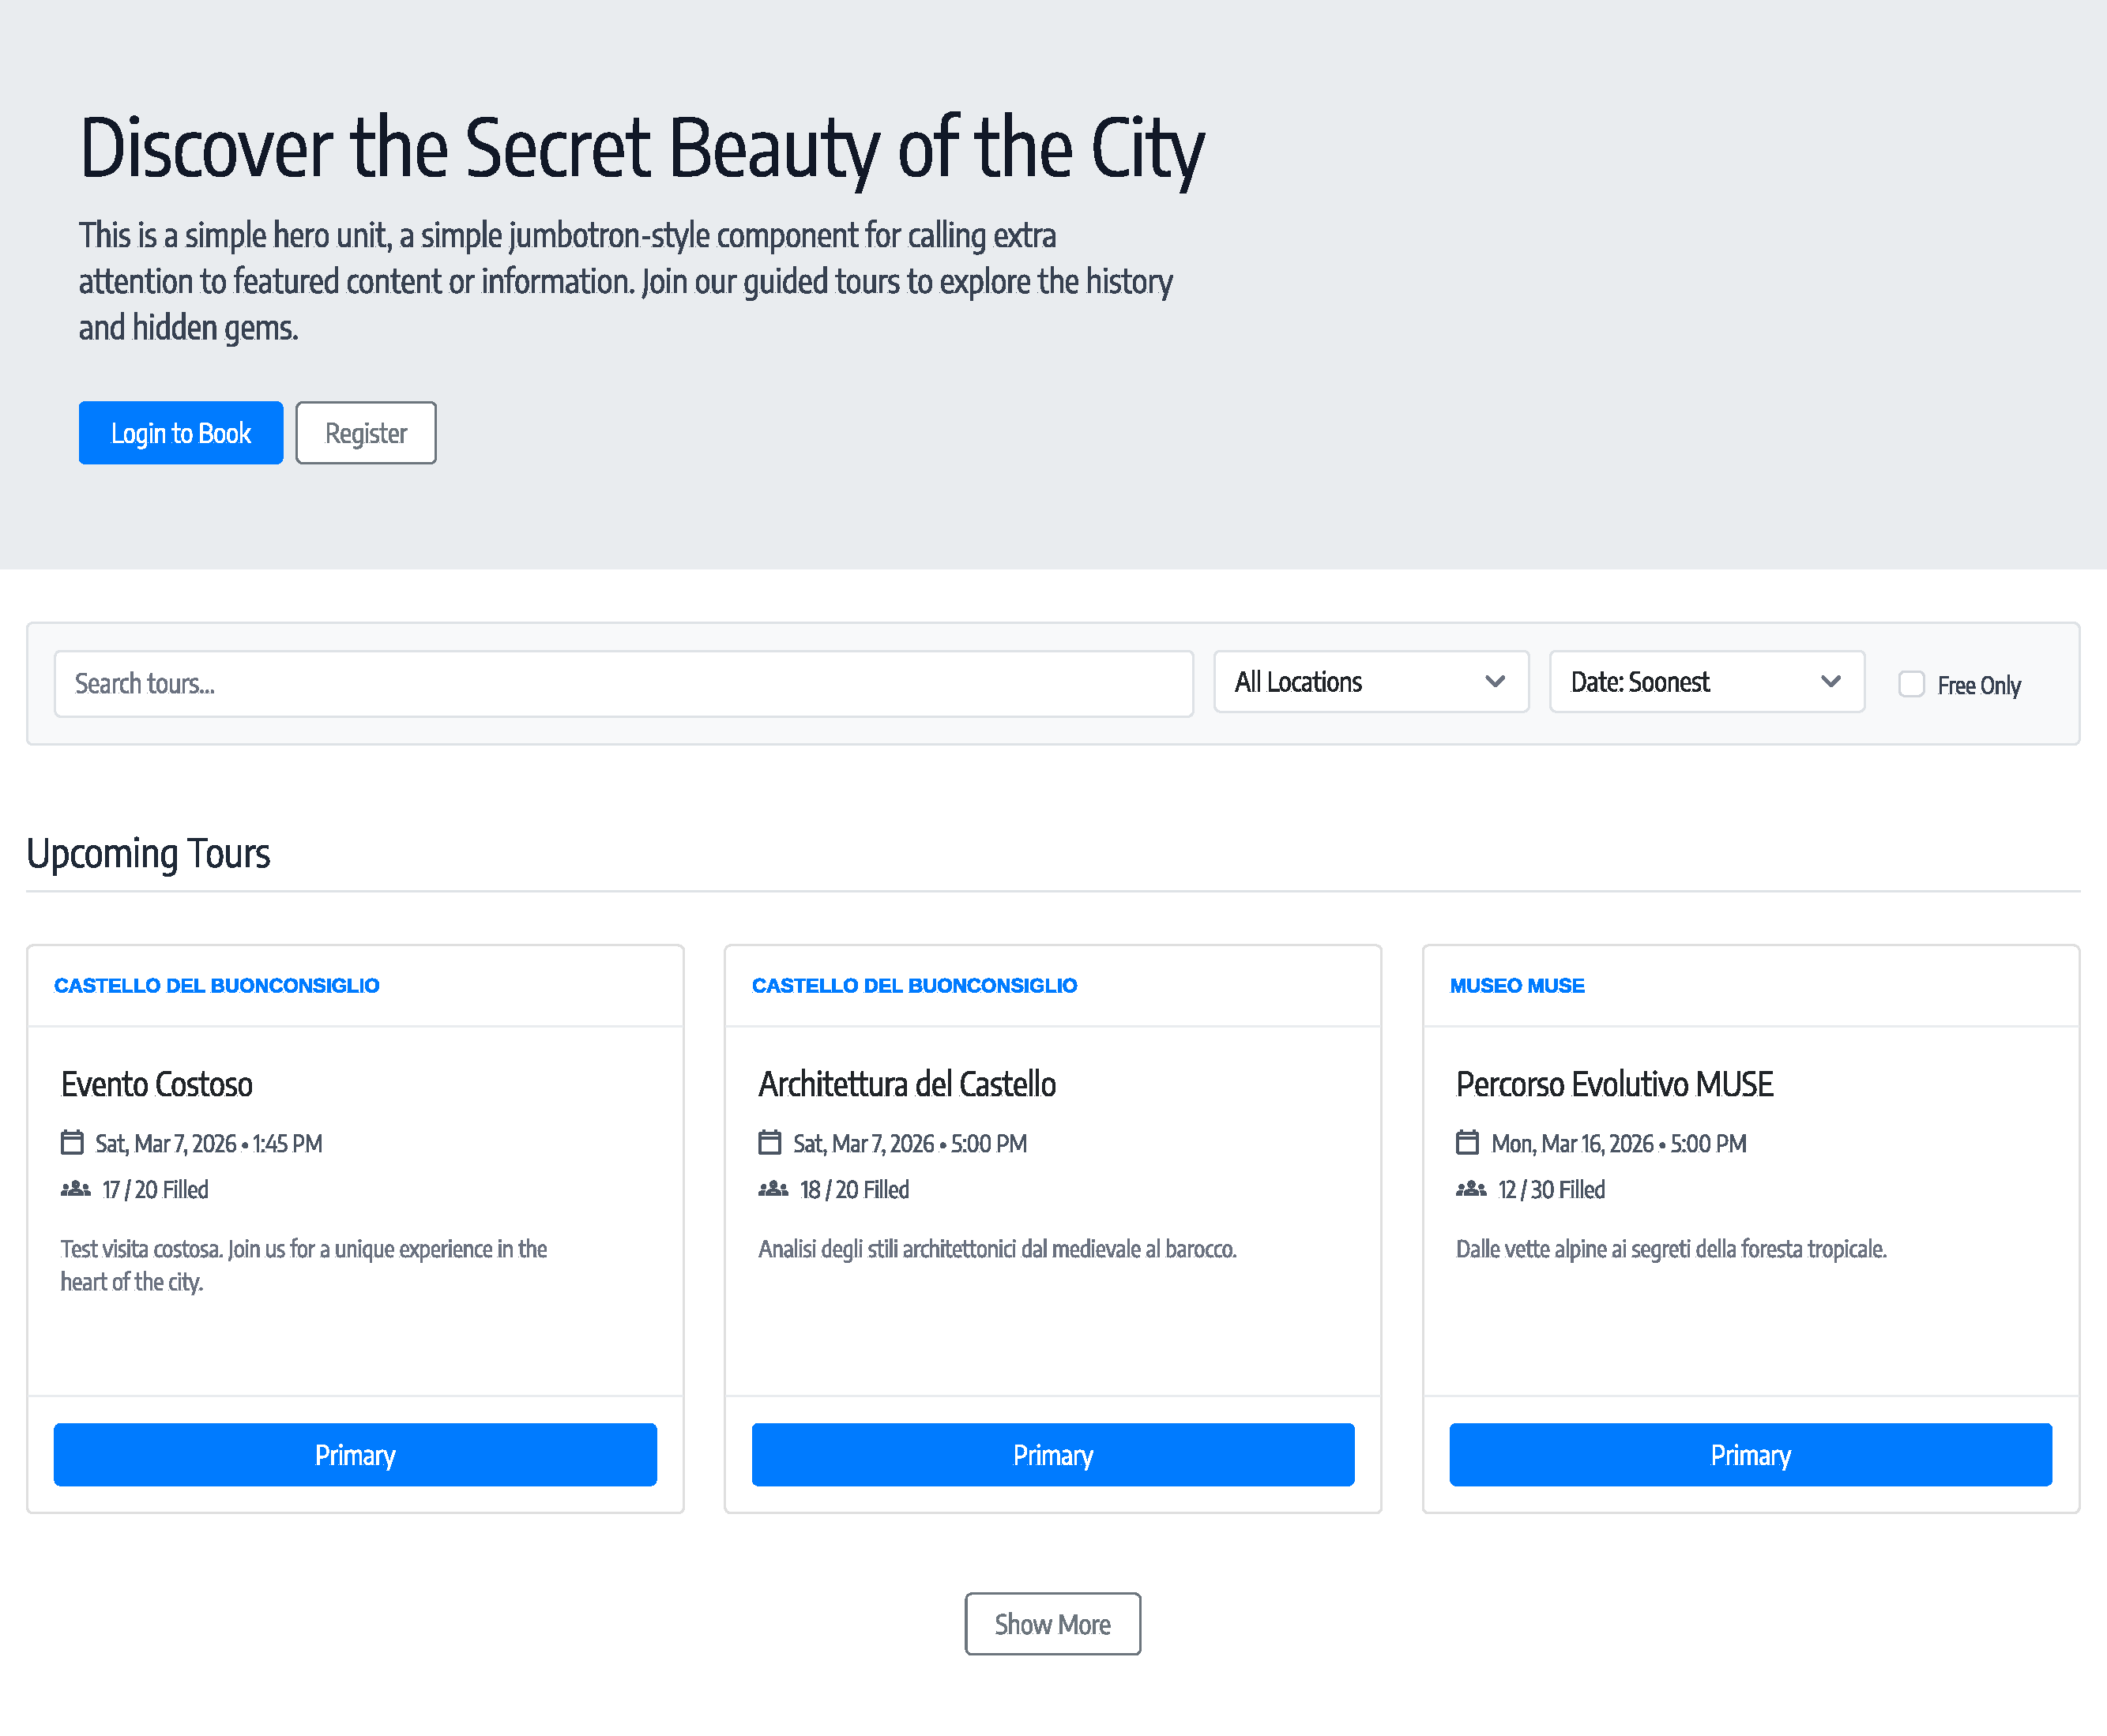
\includegraphics[width=0.9\textwidth, keepaspectratio]{capitoli/immagini/mockup/home.pdf}
    \caption{Mock-up della Home Page: il catalogo dei tour è presentato tramite card uniformi con immagine, titolo, luogo, data, posti residui e badge di stato. I filtri di ricerca (testo, distanza, gratuità) e l'ordinamento sono esposti in linea sopra la griglia, abbattendo il carico cognitivo necessario per individuare un tour di interesse.}
    \label{fig:mockup_home}
\end{figure}

% ── Mockup: Registrazione Visita ─────────────────────────────────────────────
\begin{figure}[H]
    \centering
    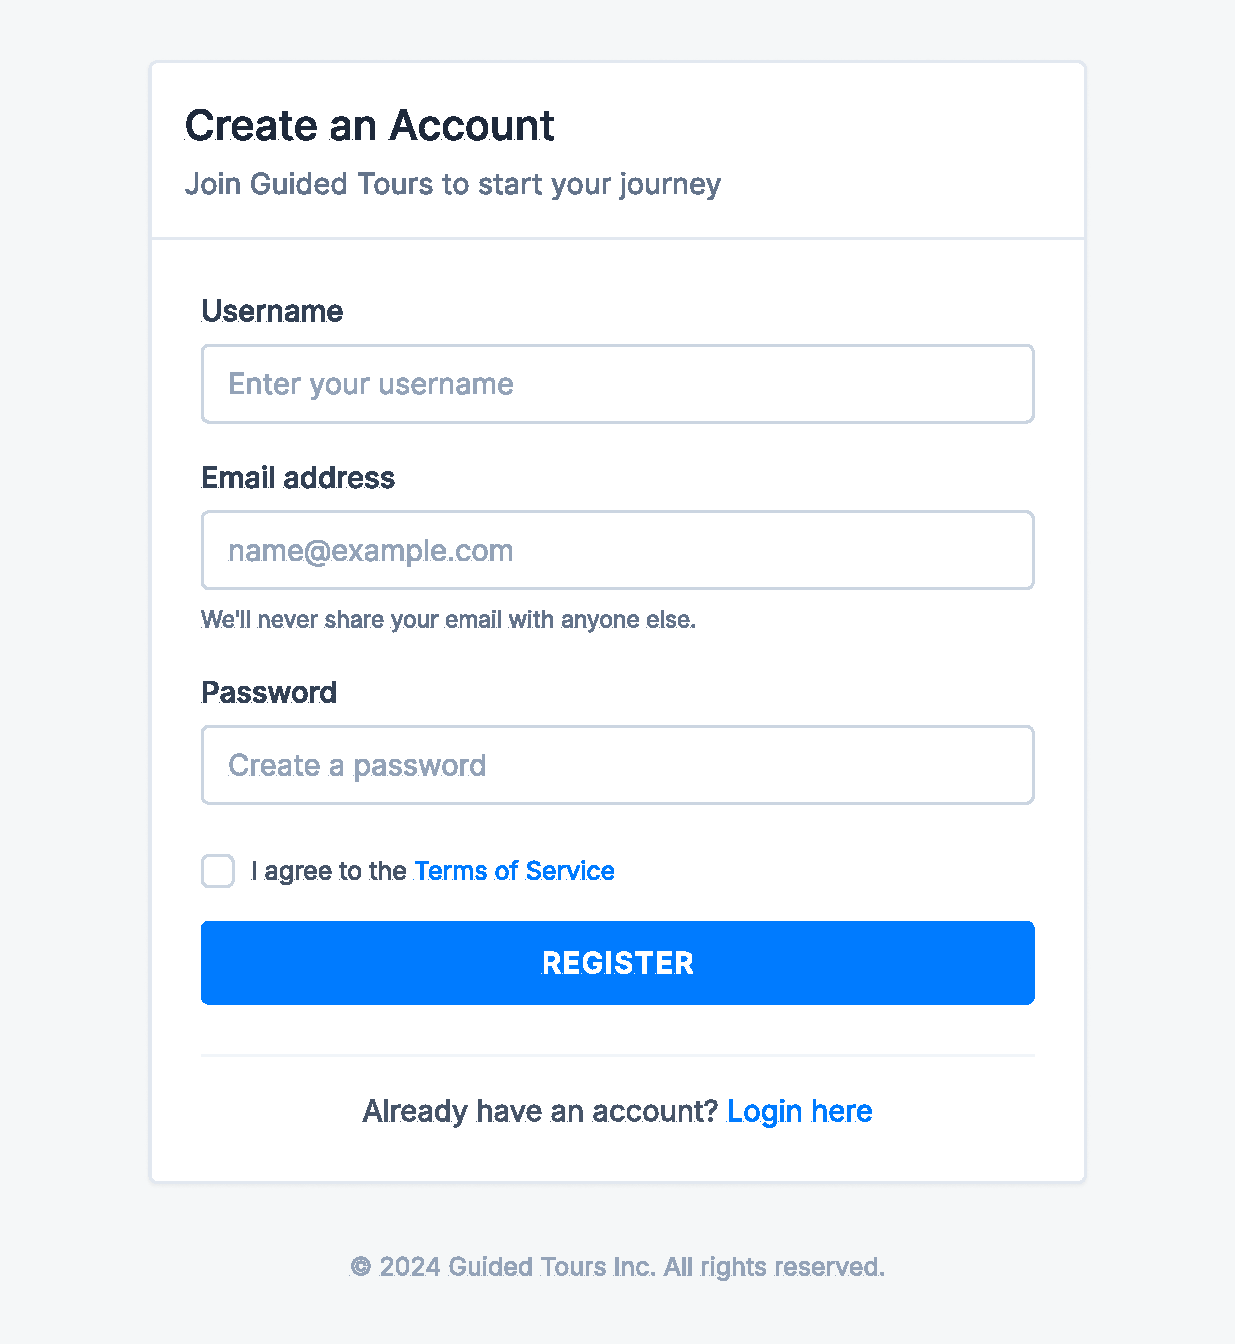
\includegraphics[width=0.75\textwidth, keepaspectratio]{capitoli/immagini/mockup/register.pdf}
    \caption{Mock-up della schermata di prenotazione visita: il modulo riepilogativo mostra il dettaglio del tour selezionato (luogo, data, prezzo, posti disponibili) affiancato al campo di selezione del numero di partecipanti. Il feedback sui vincoli (scadenza prenotazione, posti rimasti) è esposto in linea, in anticipo rispetto all'invio del form.}
    \label{fig:mockup_register}
\end{figure}

% ── Mockup: Dashboard Fruitore ───────────────────────────────────────────────
\begin{figure}[H]
    \centering
    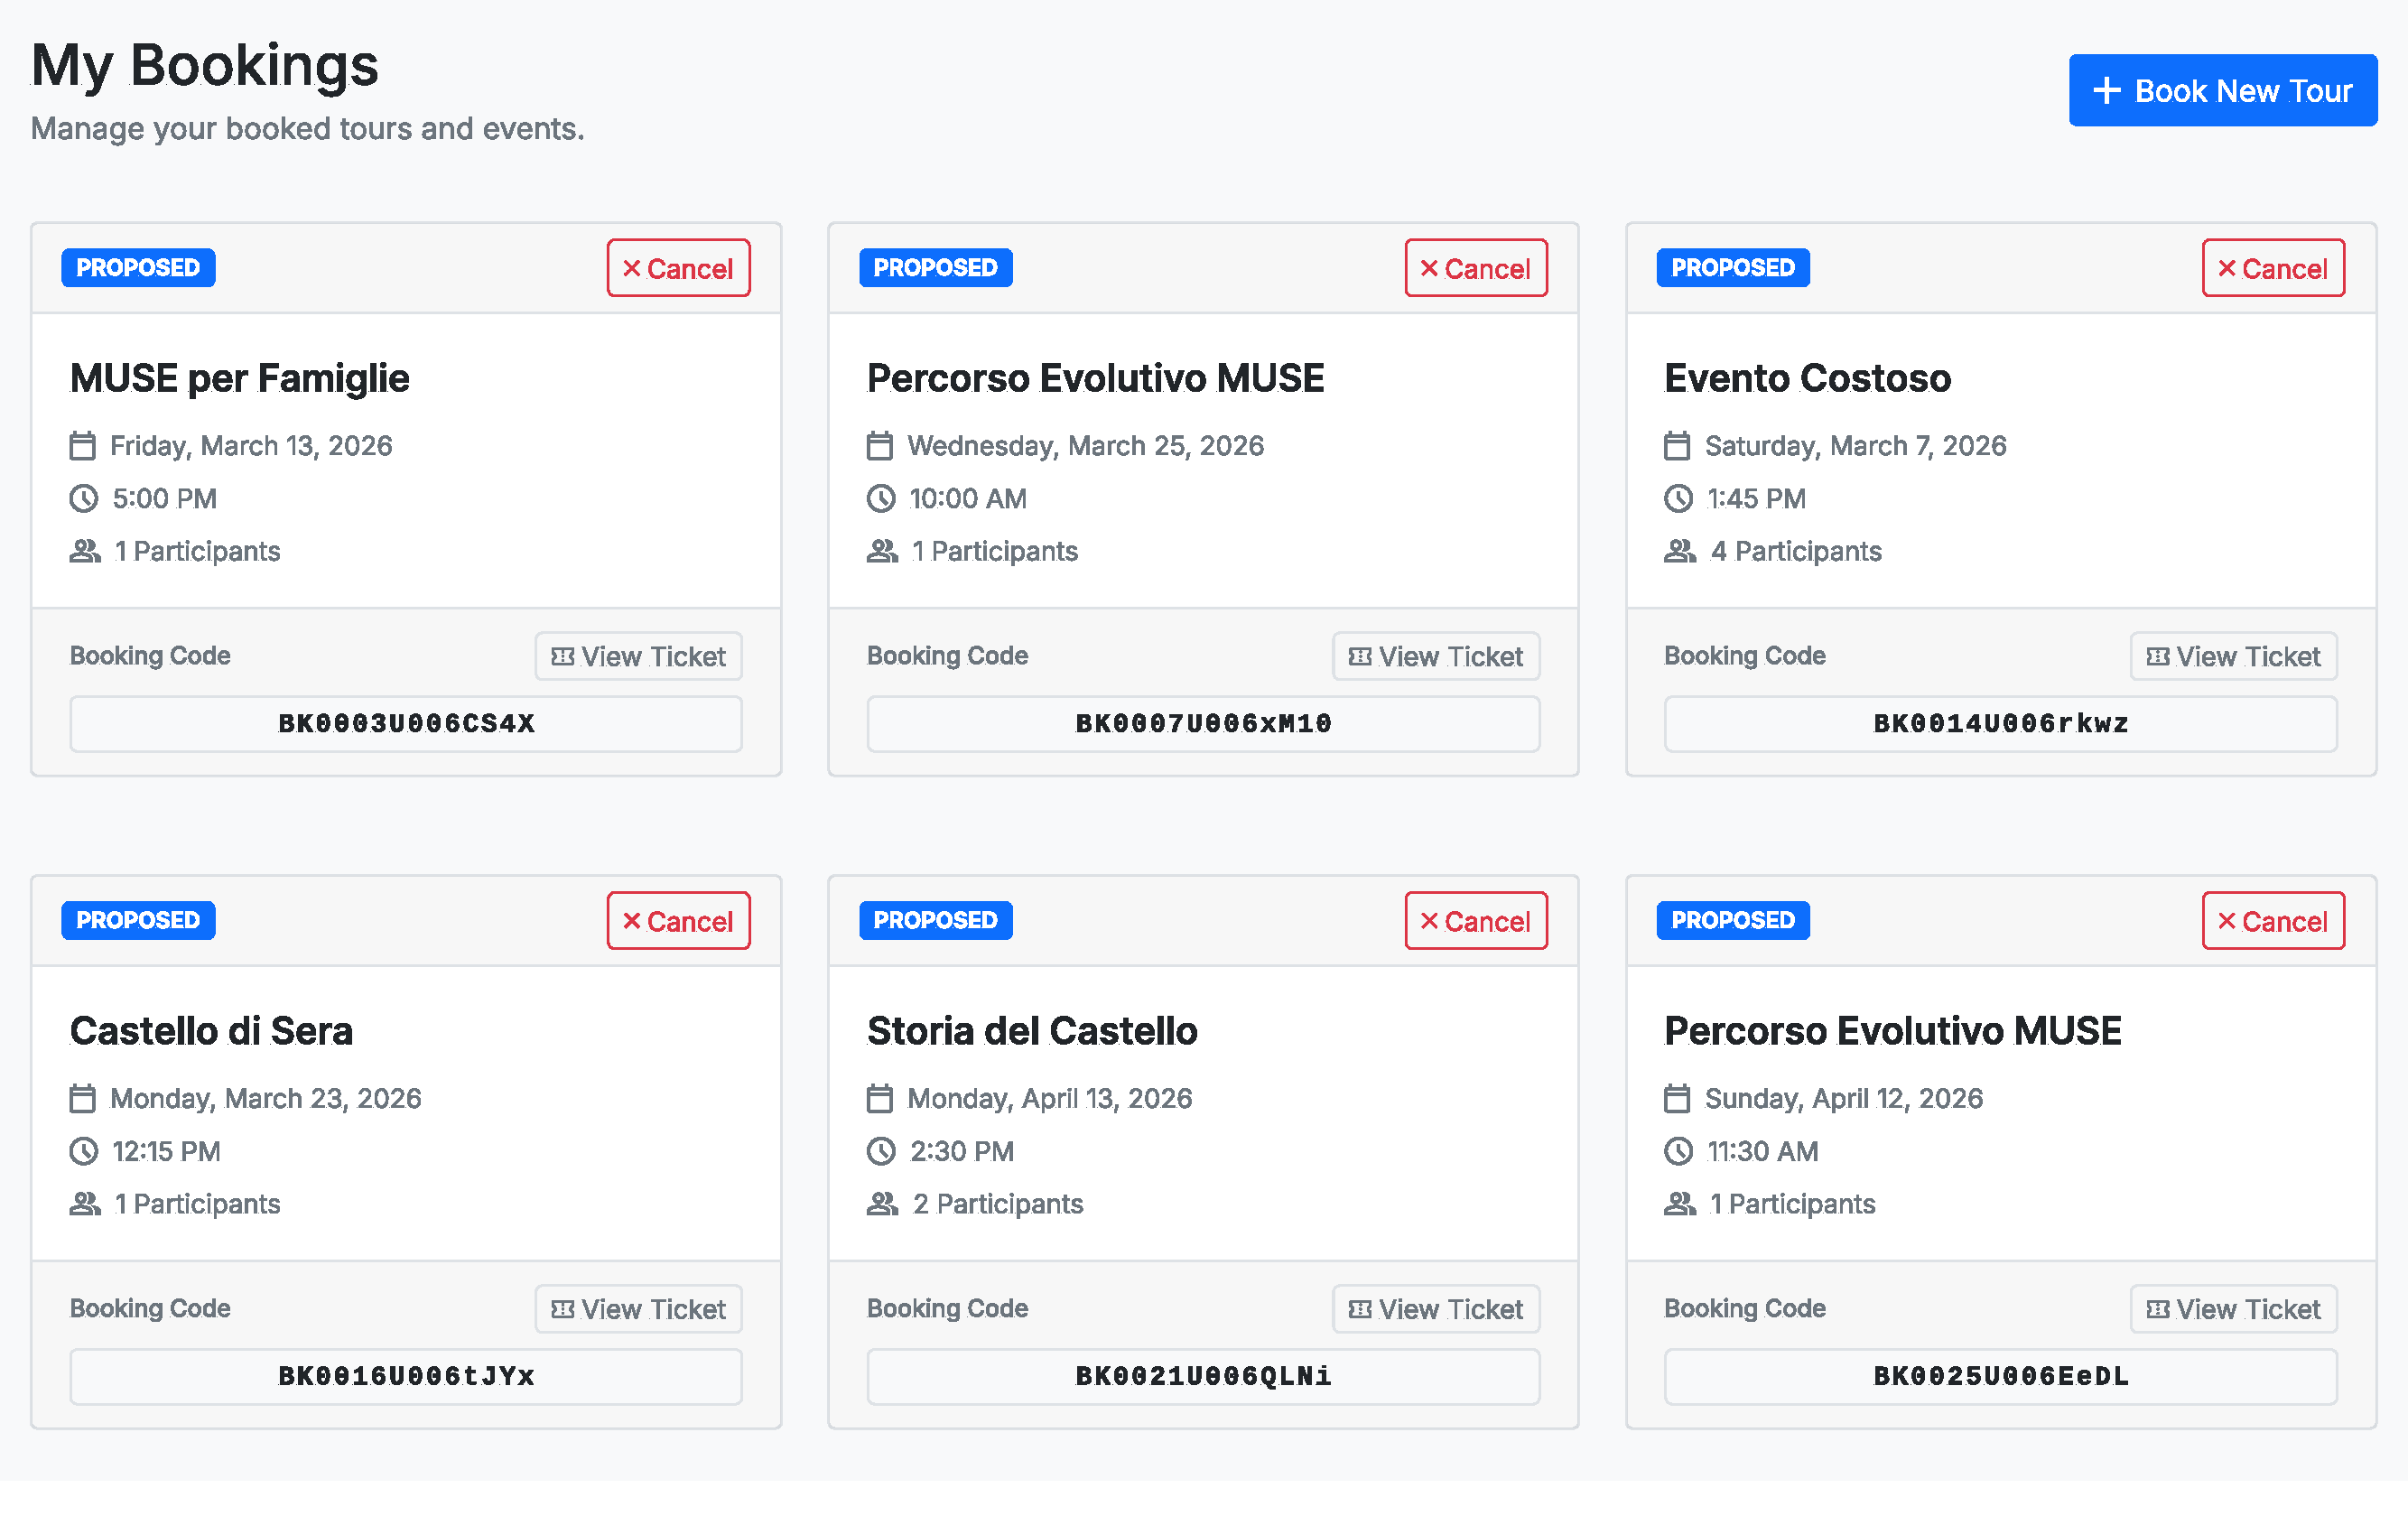
\includegraphics[width=0.9\textwidth, keepaspectratio]{capitoli/immagini/mockup/user-booking.pdf}
    \caption{Mock-up della dashboard del Fruitore — sezione prenotazioni attive: ogni prenotazione è presentata in una card che riporta il codice di prenotazione in font monospaziato, il numero di partecipanti, lo stato della visita e il pulsante di cancellazione con modale di conferma, risolvendo le problematiche di affordance e visibilità emerse nell'analisi euristica (P22, P24, P25).}
    \label{fig:mockup_user_booking}
\end{figure}

\begin{figure}[H]
    \centering
    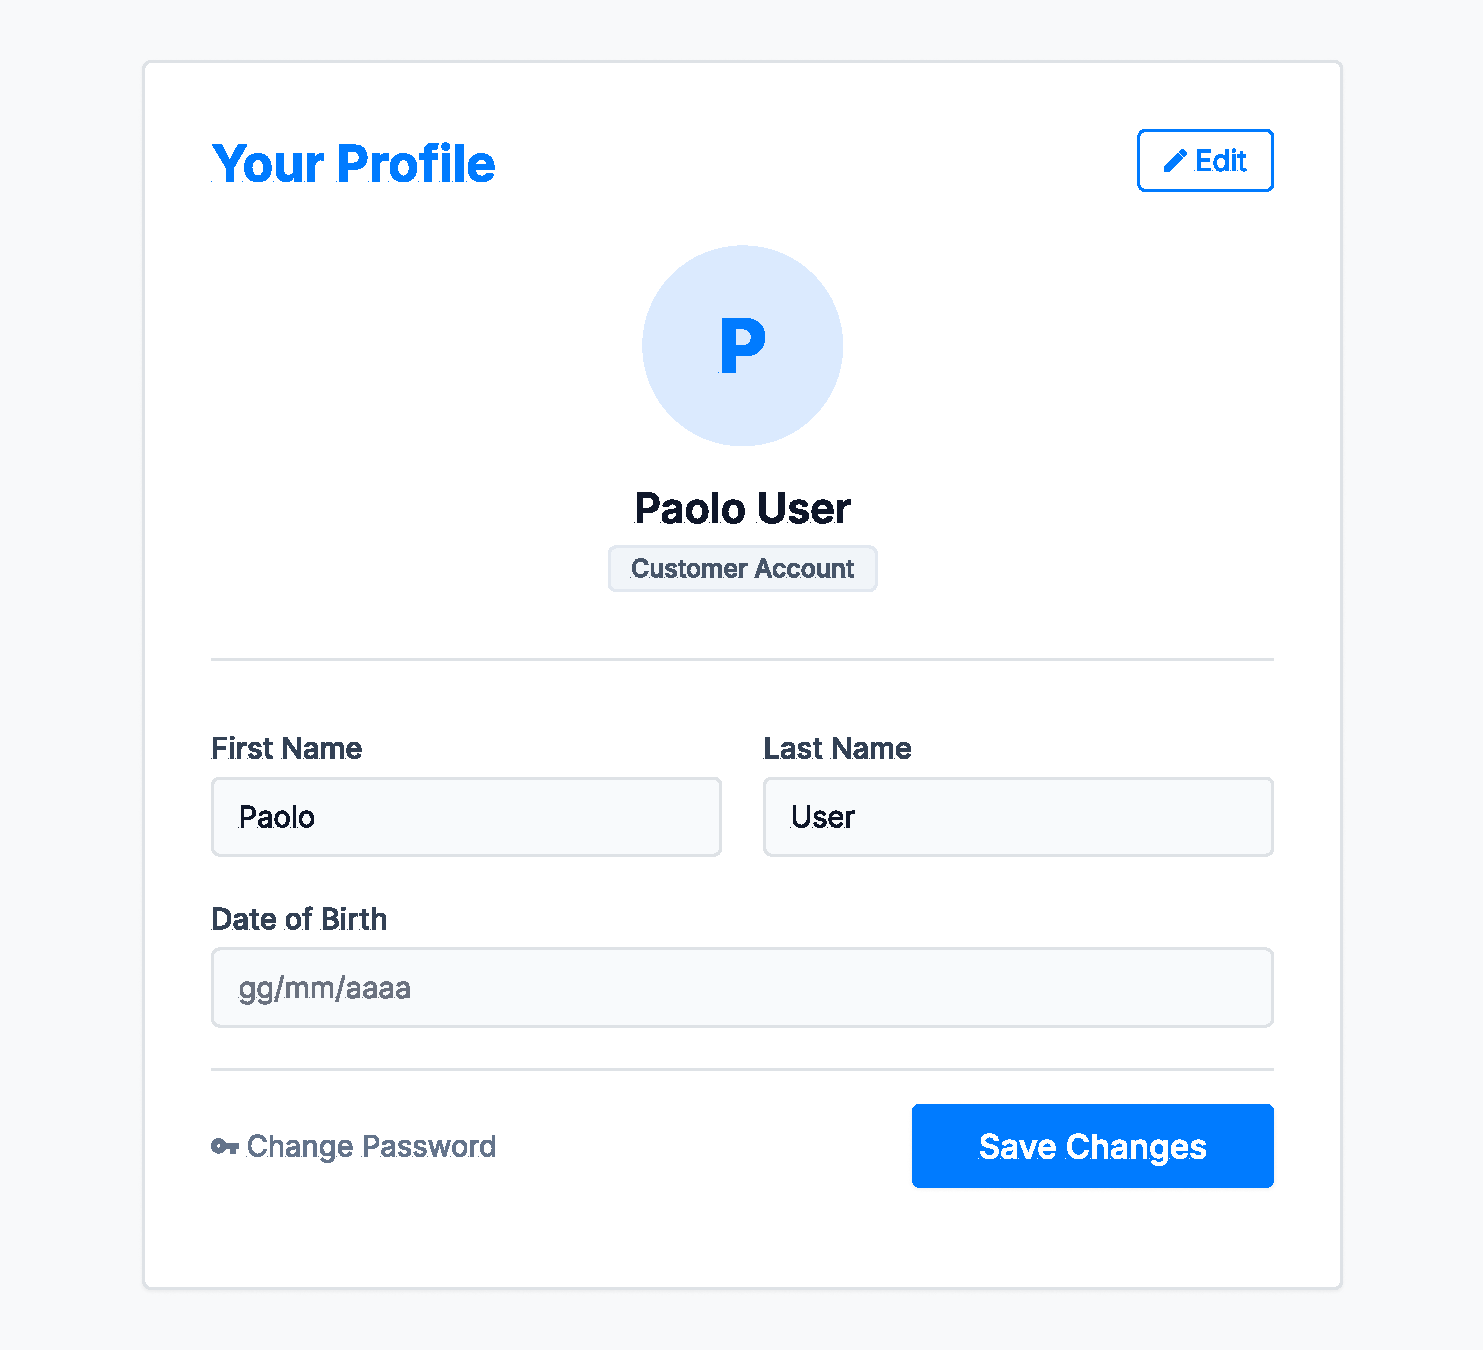
\includegraphics[width=0.75\textwidth, keepaspectratio]{capitoli/immagini/mockup/user-profile.pdf}
    \caption{Mock-up della sezione profilo utente: il pannello consente la modifica dei dati anagrafici e il cambio password direttamente dall'area personale, con validazione live dei campi e feedback semantico immediato sullo stato del salvataggio.}
    \label{fig:mockup_user_profile}
\end{figure}

% ── Mockup: Pannello Guide ───────────────────────────────────────────────────
\begin{figure}[H]
    \centering
    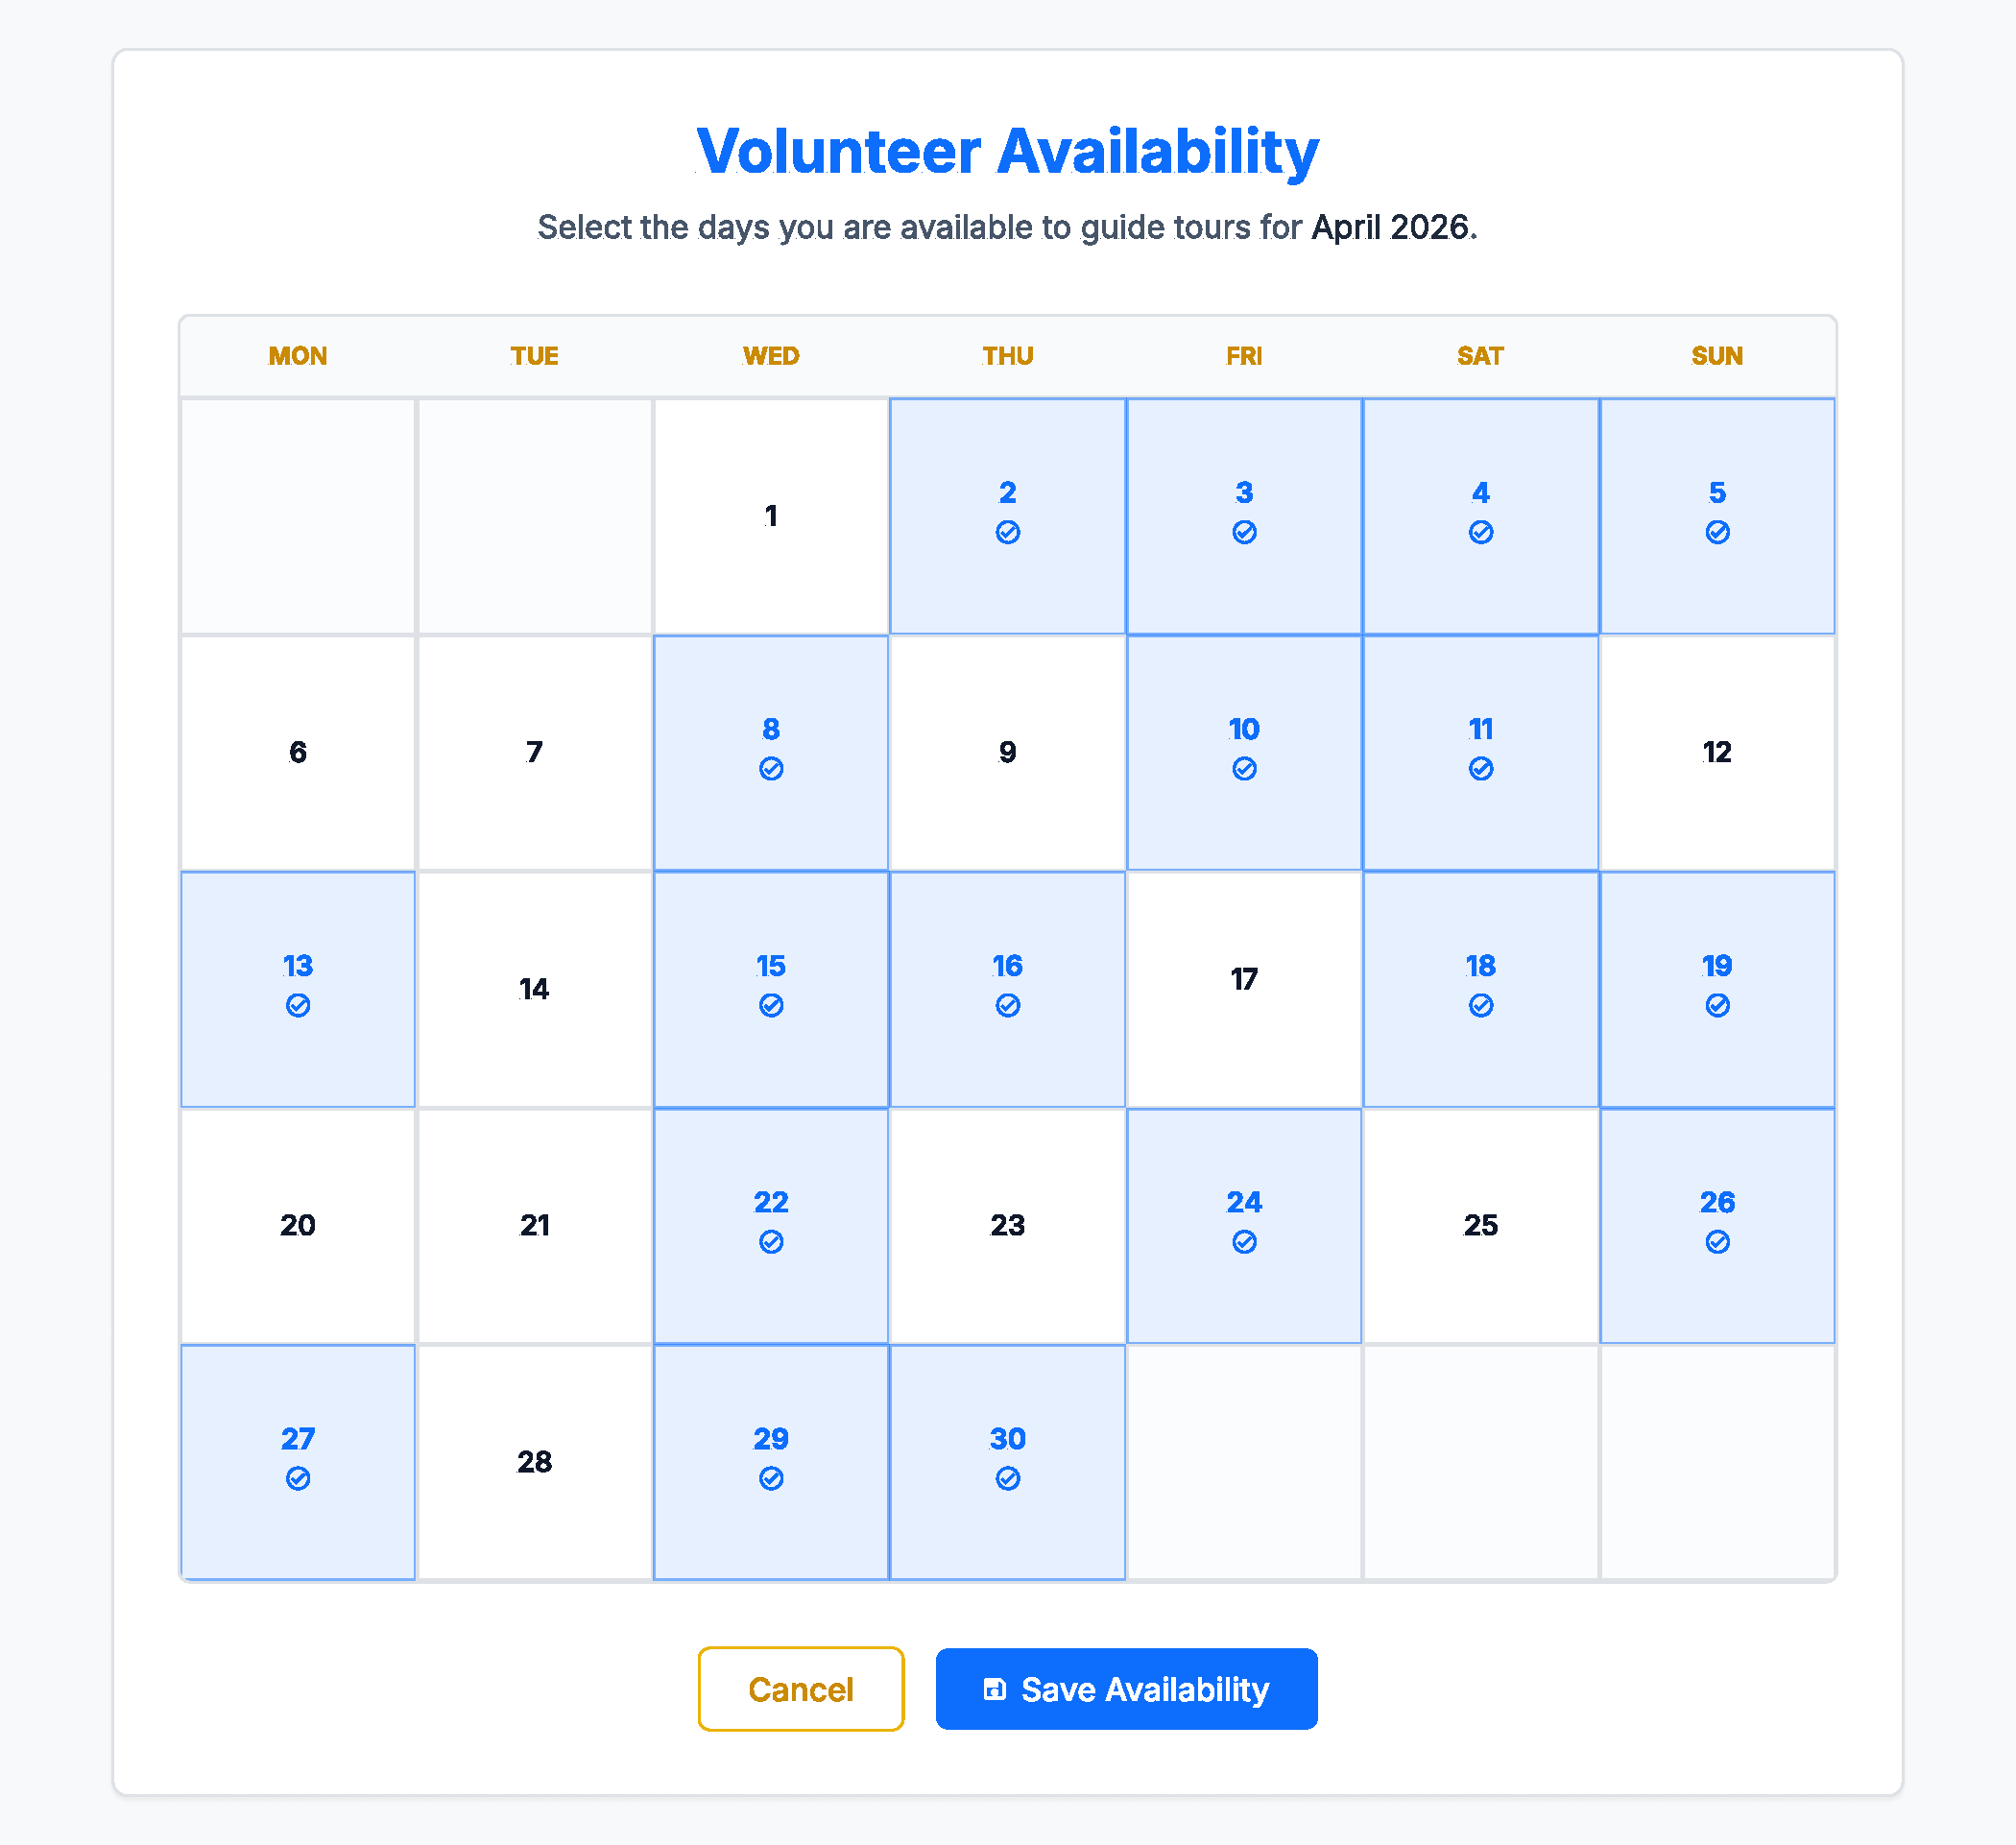
\includegraphics[width=0.9\textwidth, keepaspectratio]{capitoli/immagini/mockup/vol-availability.pdf}
    \caption{Mock-up del calendario disponibilità della Guida: la vista mensile a griglia permette di selezionare singole date o intere colonne (giorni della settimana) con un solo click, riducendo il numero di interazioni necessarie per dichiarare disponibilità ricorrenti (es. ogni sabato del mese).}
    \label{fig:mockup_vol_availability}
\end{figure}

\begin{figure}[H]
    \centering
    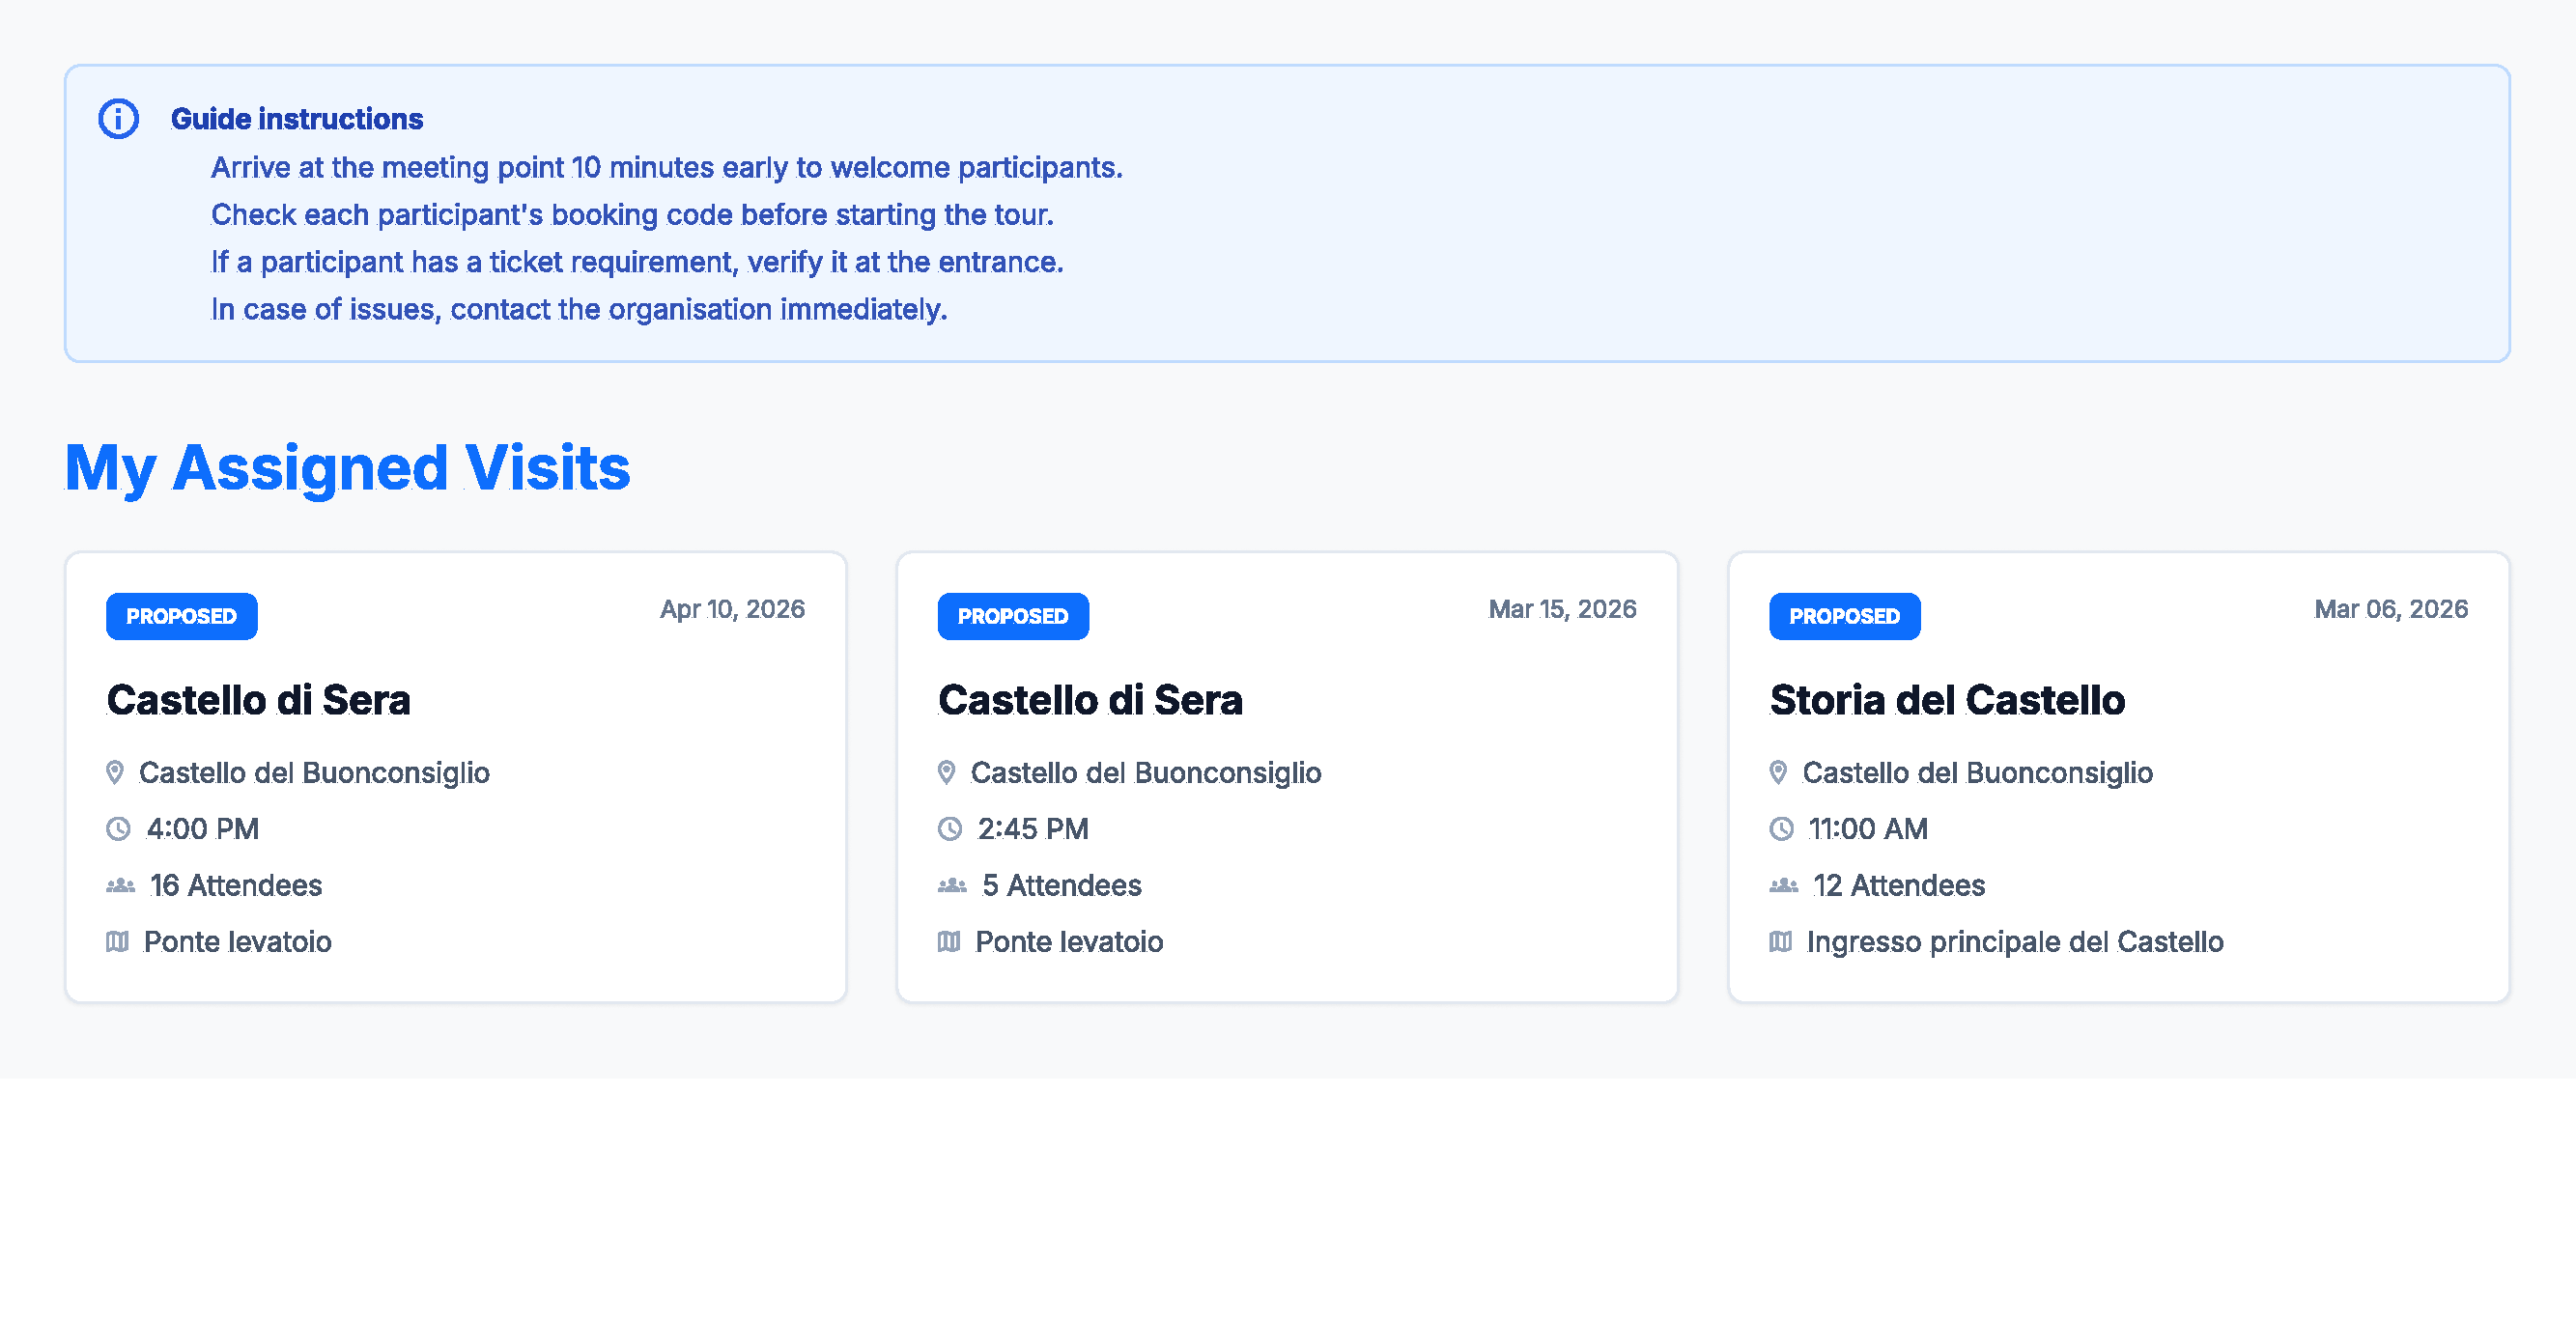
\includegraphics[width=0.9\textwidth, keepaspectratio]{capitoli/immagini/mockup/vol-panel.pdf}
    \caption{Mock-up del pannello visite assegnate alla Guida: la lista cronologica delle visite in programma espone data, luogo, numero di iscritti e stato, affiancata da un riquadro informativo con le istruzioni operative (verifica biglietti, gestione partecipanti), rispondendo alla problematica P37 relativa all'assenza di indicazioni operative contestuali.}
    \label{fig:mockup_vol_panel}
\end{figure}

% ── Mockup: Pannello Amministratore ─────────────────────────────────────────
\begin{figure}[H]
    \centering
    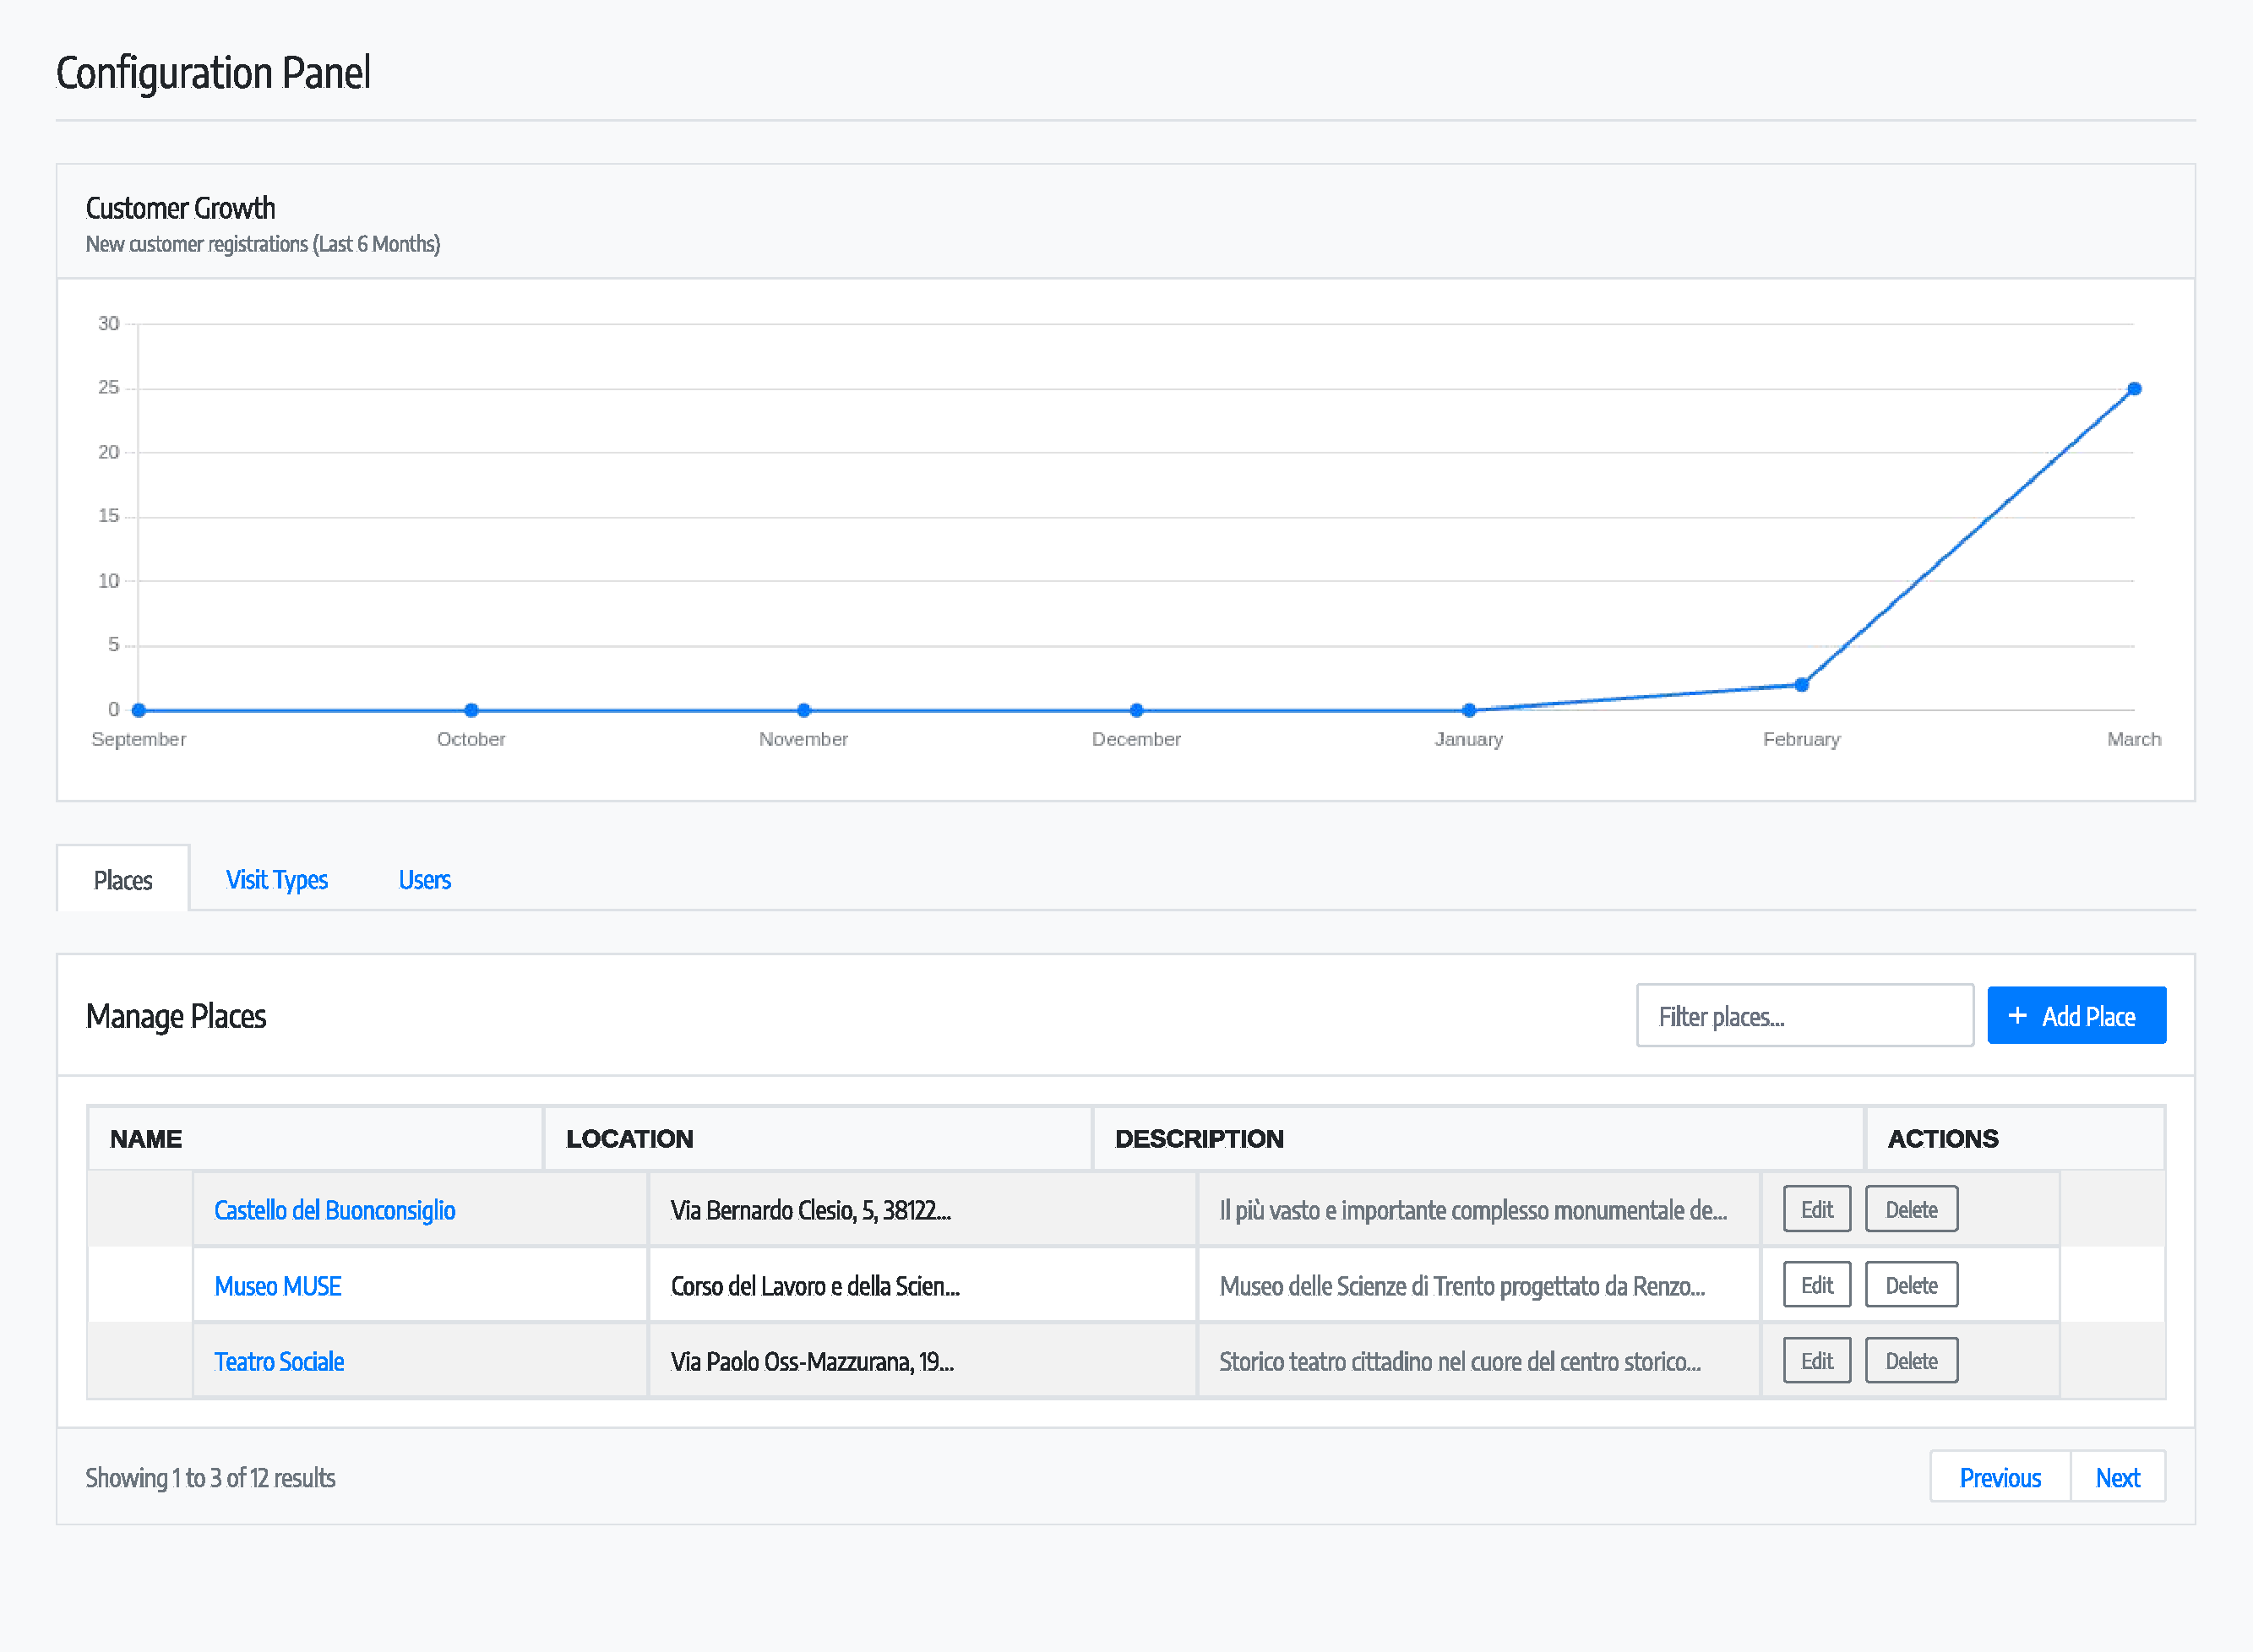
\includegraphics[width=0.9\textwidth, keepaspectratio]{capitoli/immagini/mockup/config-panel.pdf}
    \caption{Mock-up del pannello di configurazione amministratore: la sezione centralizza la gestione di utenti, luoghi e tipologie di visita in tab distinte. Il modale di eliminazione con richiesta di conferma esplicita risolve la problematica P29 (assenza di guardia prima della cancellazione), mentre la validazione in tempo reale dei campi password risponde alla problematica P28.}
    \label{fig:mockup_config_panel}
\end{figure}

\begin{figure}[H]
    \centering
    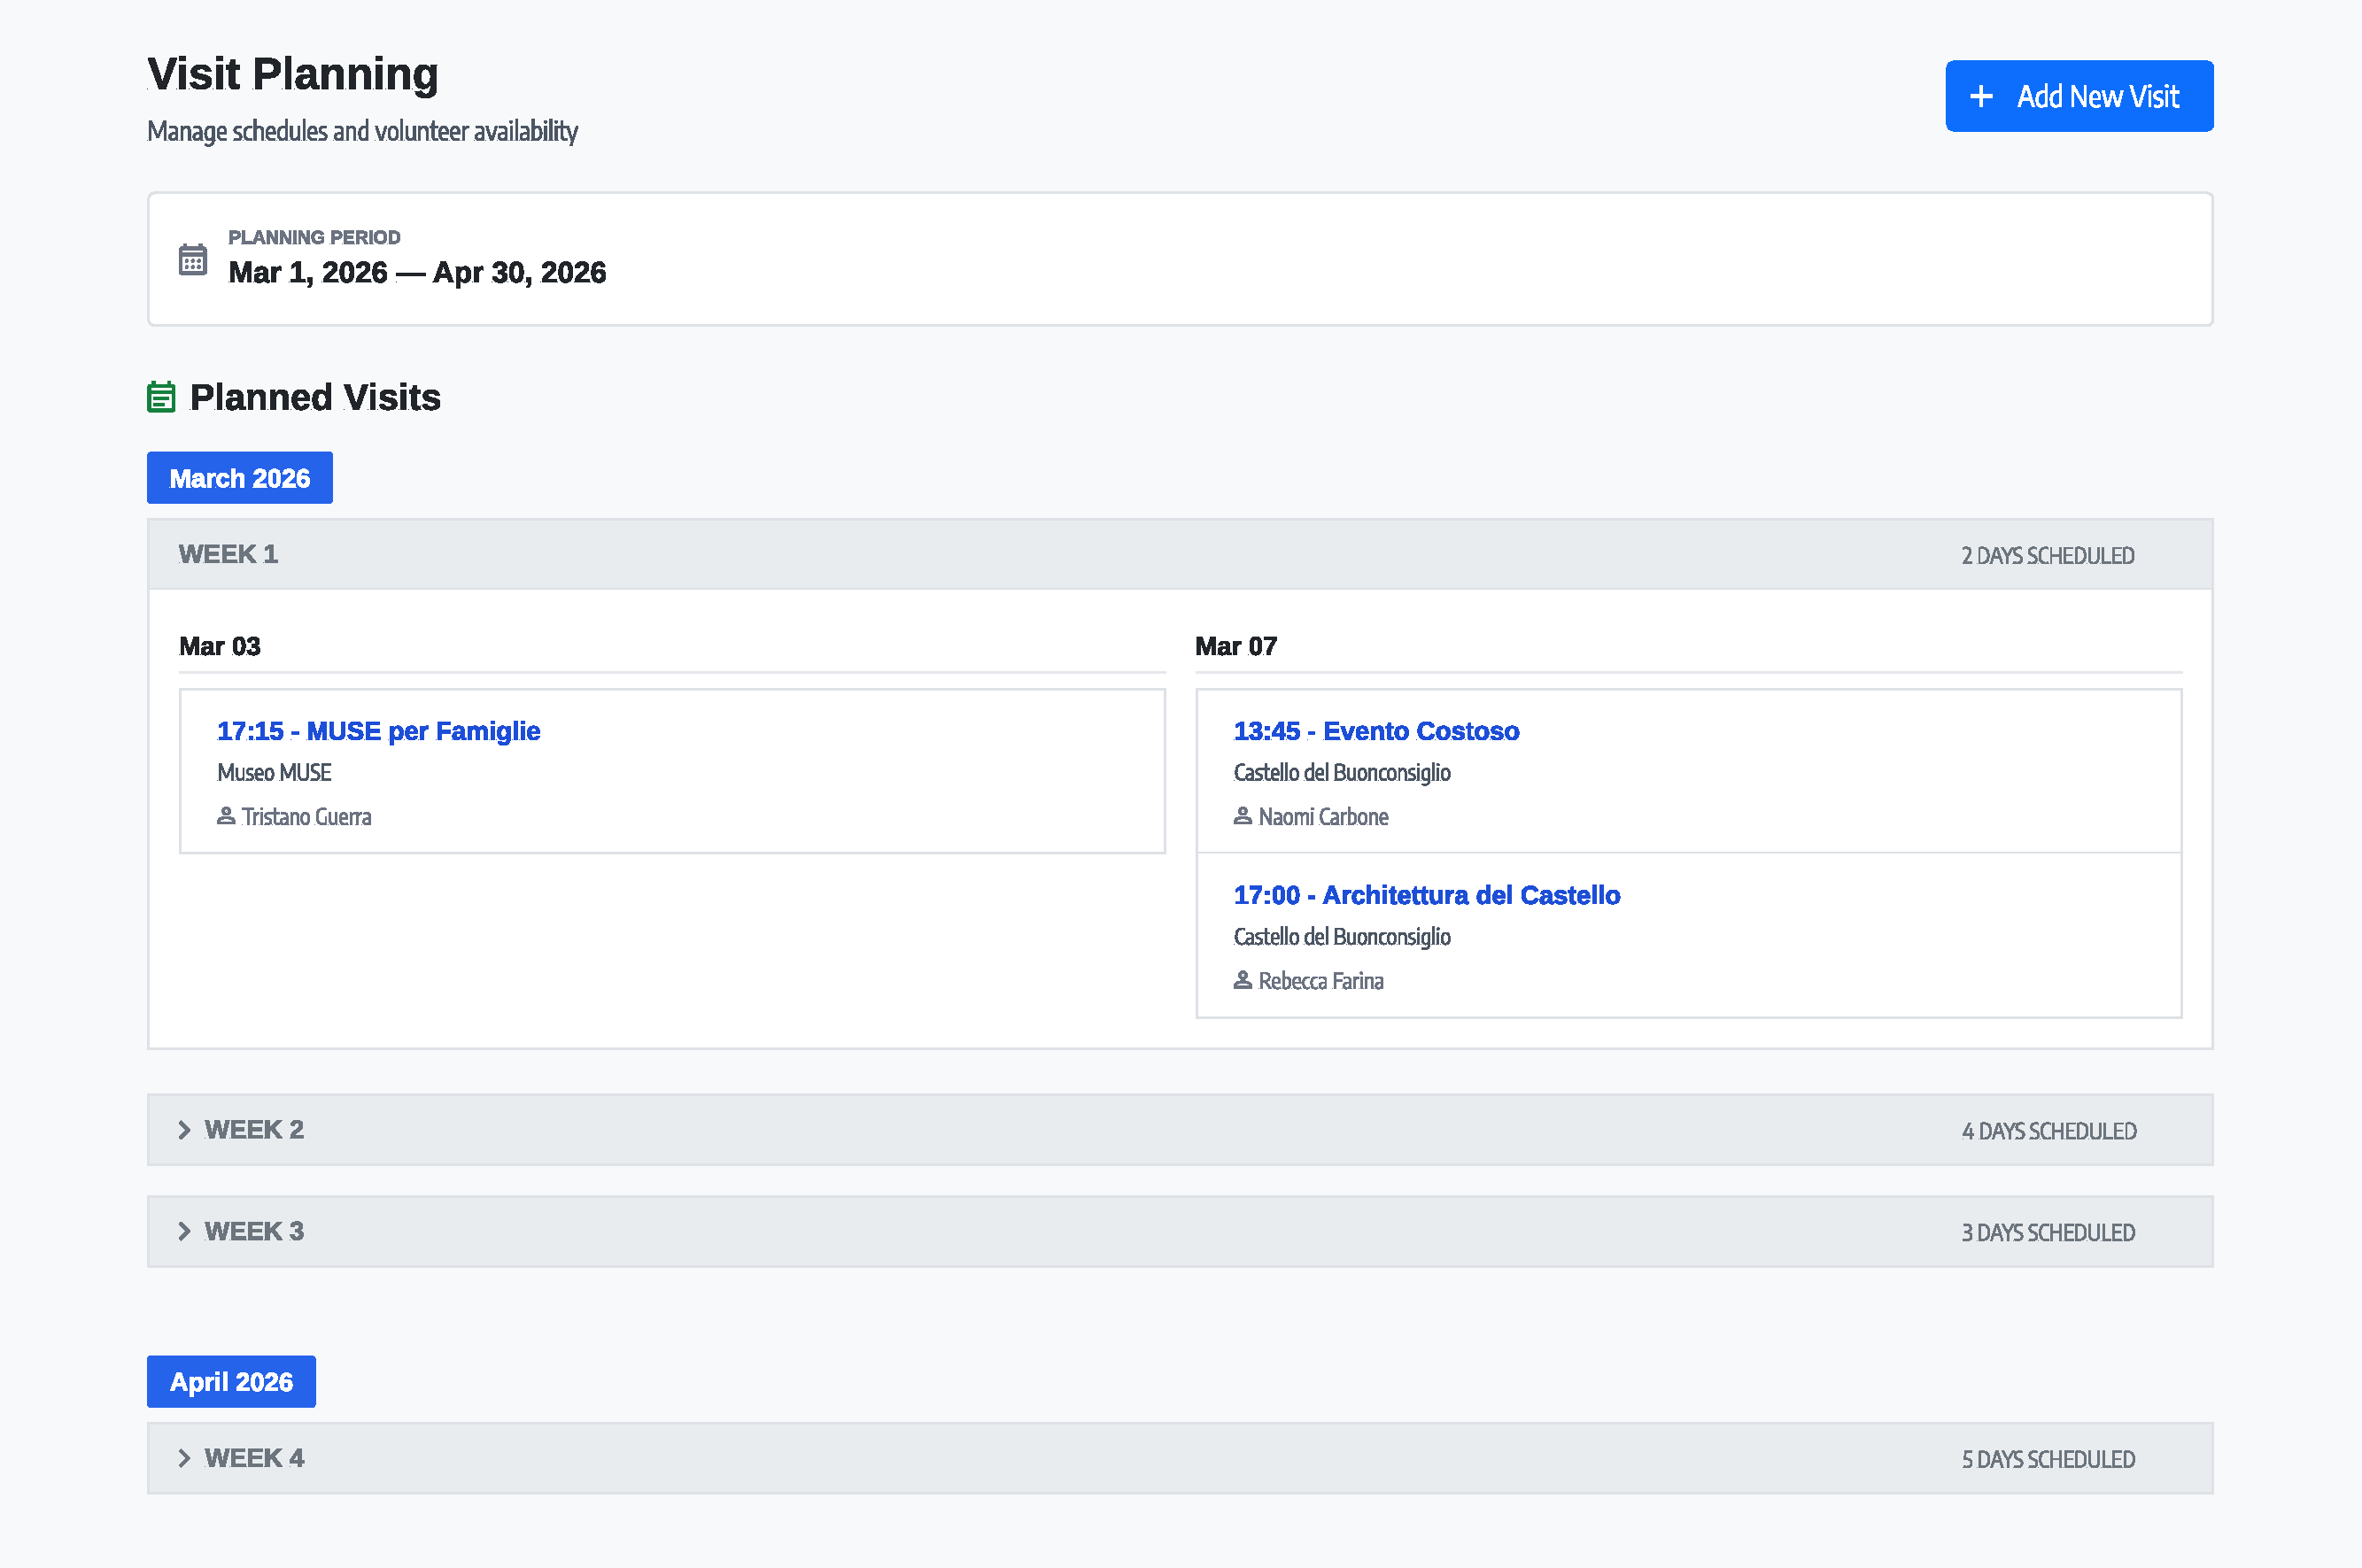
\includegraphics[width=0.9\textwidth, keepaspectratio]{capitoli/immagini/mockup/config-planning.pdf}
    \caption{Mock-up del pannello di pianificazione visite (Visit Planning): le visite sono raggruppate cronologicamente per mese e settimana, con evidenziazione cromatica dello stato (proposta, confermata, effettuata). Il flusso guidato di creazione visita — selezione tipo, data, guida disponibile — è accessibile tramite un unico pulsante contestuale, risolvendo la disorganizzazione del layout segnalata in P30 e P31.}
    \label{fig:mockup_config_planning}
\end{figure}

\subsection{Validazione Formativa dei Prototipi (Mock-up)}
Prima di procedere alla stesura del codice (coding), i mock-up ad alta fedeltà realizzati su Figma sono stati sottoposti a un meticoloso processo di validazione formativa. Il team ha adottato un approccio metodologico ibrido, diviso in due macro-fasi sequenziali, al fine di ottimizzare preventivamente l'esperienza utente.

La prima fase, di natura interna (Esperti), è consistita in un'ispezione analitica da parte del team di sviluppo. Avvalendosi del metodo del \textit{Cognitive Walkthrough}, i progettisti hanno navigato i prototipi validando la coerenza dei flussi logici (\textit{User Flows}) interattivi e verificando accuratamente il corretto posizionamento delle \textit{affordance}.

La seconda fase, di carattere esterno (Utenti finali), ha coinvolto un campione empirico ristretto di 3 individui estranei al progetto. Aderendo ai moderni dettami metodologici della \textit{Lean UX} e del \textit{Guerrilla Testing}, si è optato per una valutazione qualitativa snella. Ai partecipanti è stato chiesto di interagire liberamente con il prototipo, verbalizzando i propri ragionamenti ad alta voce secondo il celebre protocollo \textit{Think-Aloud}. La decisione di affidarsi a soli tre utenti trova solida giustificazione negli studi accademici di Jakob Nielsen, i quali dimostrano empiricamente che un campione da 3 a 5 soggetti è ampiamente sufficiente per far emergere la stragrande maggioranza delle criticità euristiche.

Questo collaudo formativo ha permesso di correggere la rotta progettuale prima di impegnare risorse nello sviluppo software (coding), demandando la misurazione statistica e oggettiva all'esperimento sommativo finale.

\section{Technical Rationale}
La risoluzione delle criticità di usabilità ha richiesto un intervento sia lato Front-end che lato Back-end. Di seguito i principali interventi tecnologici:
\begin{itemize}
    \item \textbf{Gestione del Design System}: Sebbene alcune opzioni progettuali potessero far pensare a Tailwind CSS, l'interfaccia finale è stata uniformata sfruttando appieno il framework \textbf{Bootstrap 5} unitamente a variabili SCSS customizzate (\texttt{\_variables.scss} e \texttt{app.scss}). Questo ha permesso di mantenere pulita la gerarchia del codice CSS, impiegando classi di utilità in modo mirato unicamente dove necessario.
    \item \textbf{Validazione e Feedback in tempo reale}: Il sistema sfrutta la \textbf{validazione integrata di Laravel} (tramite \texttt{\$request->validate()}) all'interno dei Controller (es. \texttt{UserController}, \texttt{AdminController}) per assicurare la robustezza dei dati. A livello di interfaccia frontale, script in \textit{Vanilla JavaScript} gestiscono messaggi di validazione live (come i controlli sulla robustezza della password nel configuratore), fornendo all'utente un feedback immediato già in fase di digitazione.
    \item \textbf{Meccanismi di conferma (Modal)}: I \textit{confirmation modals} per le azioni distruttive, al posto di impiegare librerie più pesanti come Livewire, sono stati realizzati tramite \textbf{Modali Bootstrap} nativi interfacciati con script JavaScript centralizzati. Questo rende più performante la pagina: uno script globale cattura l'evento, estrae dinamicamente i parametri utente/oggetto (\texttt{data-action}, \texttt{data-item-name}) e inserisce i dati prima della visualizzazione del modale, garantendo modularità.
\end{itemize}

\section{Reverse Engineering e Documentazione del Visual Design dal Codice}
Il restyling grafico ha posto forte enfasi sull'accessibilità, cercando di risolverne un difetto di base emerso nell'analisi. Attraverso il \textit{reverse engineering} dei fogli di stile customizzati (file \texttt{\_variables.scss} e \texttt{app.scss}) e dei template base dell'interfaccia (es. \texttt{app.blade.php}), è possibile mappare formalmente i principi di visual design adottati nel sistema.

\subsection{Psicologia e Gerarchia del Colore}
La palette cromatica estratta dal codice definisce una gerarchia visiva basata su un forte contrasto, progettata per bilanciare l'aderenza all'estetica istituzionale con l'usabilità:
\begin{itemize}
    \item \textbf{Primario (Vibrant Blue, \#0d6efd):} Impiegato per le azioni principali (\textit{call-to-action}) e le direttive di navigazione primaria. Comunica sicurezza e grande affidabilità professionale.
    \item \textbf{Secondario e Accento (Amber/Gold, \#ffc107):} Riservato per le notifiche di avviso (\textit{warning}) o per polarizzare focalmente l'attenzione visuale in contesti con alta densità informativa.
    \item \textbf{Feedback Semantico (Success \#198754, Danger \#dc3545, Info \#0dcaf0):} Il frontend sfrutta sistematicamente questa sintassi cromatica universale per i \textit{Live Input Feedback} (es. form validation) e per marcare le alterazioni critiche dello stato (es. i \textit{Global Delete Modal} in rosso), abbattendo i tempi di ricezione cognitiva degli esiti di sistema.
    \item \textbf{Colori Neutri e Tema Scuro:} Le variabili architetturali \texttt{--bs-body-bg} (\#121212) e \texttt{--card-bg} (\#2a2a2a) presenti nel blocco nativo del tema \textit{dark} dimostrano una stratificazione atta a sopprimere l'affaticamento oculare (\textit{eye-strain}). Viene adoperato un grigio antracite al posto del nero assoluto, esaltando otticamente il volume del componente sollevato rispetto al fondale. Vi si accavallano filtri traslucidi (\textit{glassmorphism} settato all'85\% di opacità, es. \texttt{rgba(42, 42, 42, 0.85)}) che permettono ai layer di compenetrarsi organicamente.
\end{itemize}

\subsection{Tipografia e Leggibilità}
Dall'ispezione della dichiarazione centrale globale (\texttt{\$font-family-sans-serif}), emerge primariamente l'utilizzo dell'innovativa famiglia tipografica \textit{Outfit} (importata via \textit{Google Fonts}) e del successivo \textit{system stack}. Si tratta di un \textit{sans-serif} geometrico assai limpido, leggibile a qualsivoglia scalatura *viewport*.

La gerarchia dei pesi è decisa sincreticamente all'adozione delle utility del framework (\texttt{display-4}, \texttt{h3}, \texttt{h5}), abbinate per la titolazione ad un peso netto e consistente (\texttt{\$headings-font-weight: 600;}). Scelte del genere irrobustiscono e incanalano efficacemente lo \textit{scanning pattern} oculare rapido (stile F-Pattern), demarcando con solida incisività il perimetro visivo della \textit{hero section} dai normali blocchi testuali più analitici di un \textit{body} classico.

\subsection{Spaziature e Principi della Gestalt}
Le logiche strutturali CSS di \textit{Guided Tours} e i costrutti formali del layout adottati traslano in codice i fondamenti pervasivi dettati dalla psicologia della forma (\textit{Gestalt}):
\begin{itemize}
    \item \textbf{Prossimità e Regione Comune:} L'impiego pervasivo di \texttt{.card} dotate di raggiature accentuate (\texttt{border-radius: 1rem}) unito a background cromaticamente scissi (\texttt{--card-bg}), delimita materialmente insiemi eterogenei in una sola "regione comune" raggruppata logicamente. La separazione visiva è amministrata da una netta abbondanza di padding regolari (\texttt{py-5}, \texttt{gap-2}) che disaccoppia entità estranee alleggerendone drasticamente la tensione di decifrazione (\textit{Legge della Prossimità}).
    \item \textbf{Feedback Tattile Implicito (Buona Continuazione):} Le tessere (\textit{Cards}) accolgono micro-transizioni reattive (\texttt{.card-hover:hover}) che traducono un istantaneo vettore verticale di elevazione (\texttt{translateY(-8px)}), associato ad intensificazione dell'ombra (\textit{drop-shadow}). Tali riscontri tridimensionali emulano solide affordance del mondo fisico, canalizzando per implicita continuazione visiva le scelte esplorative e il rassicurante cliccaggio dei dispositivi di input dell'internauta.
\end{itemize}

\section{Design Pattern d'Interazione (HCI)}
L'interfaccia è stata costruita assemblando diversi Design Pattern consolidati nella Human-Computer Interaction, al fine di garantire familiarità, ridurre il carico cognitivo e accelerare la curva di apprendimento per i diversi profili utente presenti nel vario panorama del progetto:
\begin{itemize}
    \item \textbf{Cards (Schede Visive)}: Impiegate massicciamente nella \textit{Home Page} per raggruppare coerentemente i metadati di ogni singolo tour (titolo, data, luogo, posti disponibili). Questo pattern astrae la complessità del database in blocchi visivi scansionabili e logicamente isolati, ideali per la fruizione mobile e per l'immediatezza cognitiva.
    \item \textbf{Navigation Tabs (Pannelli a schede)}: All'interno dell'area \textit{Admin Configurator}, la gestione di "Places", "Visit Types" e "Users" è organizzata in sezioni a tabulazione. Ciò elimina il \textit{page refresh} continuo e compatta le opzioni amministrative critiche in un'unica plancia, ottemperando all'euristica del design estetico minimalista senza eccessivo rumore visivo.
    \item \textbf{Global Navigation Bar (Menu Persistente)}: Una barra di navigazione fissa posta al vertice funge da àncora di salvataggio e di orientamento perpetuo per l'utente. Rende costantemente accessibili i link operativi determinanti (Home, Accesso, o Dashboard personale) prescindendo dal grado di scorrimento verticale.
    \item \textbf{Faceted Search \& Filter Bar}: Pattern primario inserito nella \textit{Home Page} a favore del \textit{Fruitore}. Permette di modulare dinamicamente i risultati (filtro per luogo, stringa testuale, ordine temporale o scrematura dei costi), snellendo il tempo di scoperta e trasmettendo il senso di controllo e libertà d'azione.
    \item \textbf{Visual Status Badges (Codifica semantica a etichette)}: Guidato dalla nuova palette cromatica del sistema, l'impiego di tag "pill" compatti (come "Open", "Imminent" per le visite, oppure i tag dei ruoli amministrativi) restituisce una profilazione visiva in una frazione di secondo. Alimenta il principio di \textit{recognition rather than recall}.
    \item \textbf{Confirmation Trigger (Modali antierrore distruttivo)}: Al fine di prevenire errori di esecuzione involontari (\textit{slips}) durante le operazioni di Backoffice (es. l'annullamento di risorse storicizzate o la rimozione di un volontario), è stato introdotto un meccanismo di controllo preventivo. L'interfaccia intercetta l'azione distruttiva attraverso un "Global Delete Modal", costringendo così l'utente a validare l'azione in modo esplicito e consapevole ("This action cannot be undone").
    \item \textbf{Continuous / Asynchronous Scrolling (Load More)}: Rispetto a un'impaginazione classica tradizionale, che potrebbe frammentare l'esplorazione, l'utilizzo di un pattern asincrono incrementale per l'elenco dei tour consente una navigazione progressiva nel catalogo, mantenendo sempre visibili e accessibili l'header e il form dei filtri.
    \item \textbf{Live Input Feedback (Validazione Contestuale)}: Questo pattern è implementato nei form critici per comunicare istantaneamente il rispetto o la violazione dei vincoli strutturali (es. i requisiti di robustezza della password). Fornendo un feedback in tempo reale, si riduce la frustrazione tipicamente associata agli errori di validazione notificati solo in fase di sottomissione (Submission Postponed Errors). 
\end{itemize}

\section{Role-Based Customization: Le 4 Home Page}
Per assecondare le diverse personas documentate in fase esplorativa, la Home Page (\texttt{home.blade.php}) agisce come smistatore univoco. Adatta infatti il suo layout e le proprie funzionalità in tempo reale basandosi sull'autenticazione tramite direttive di autorizzazione:
\begin{enumerate}
    \item \textbf{Guest (Visitatore Anonimo)}: Accolto da messaggi esplorativi con orientamento alla conversione, che invitano l'utente a registrarsi oppure a loggarsi ("Login to Book") per intraprendere un'esperienza guidata.
    \item \textbf{Customer (Fruitore)}: Visualizza pulsanti interattivi ("Browse Tours") per ispezionare istantaneamente il catalogo delle visite, unitamente ad uno shortcut persistente che rimanda alla "My Dashboard" per tenere d'occhio i biglietti.
    \item \textbf{Volunteer (Guida)}: Viene informato sin dalla prima riga a procedere all'interno della sua area specifica, al fine di impostare la propria personale disponibilità settimanale per l'abbinamento ai tour.
    \item \textbf{Admin (Configuratore)}: L'interfaccia muta in una plancia direzionale limitando le grafiche superflue; il testo guida l'amministratore e gli offre accesso rapido alla visualizzazione delle iscrizioni in aumento e alle statistiche base.
\end{enumerate}

\section{Feature Breakdown}

\subsection{Sistema di Filtering e Sorting dinamico}
Sulla Home Page pubblica, il pannello di ricerca esplorativo che correda la lista dei tour integra funzioni multiple: ricerca testuale live, filtro sulla località, vincolo sul costo ("Free Only") ed un selettore di ordinamento (temporale o alfabetico). Questa architettura è pilotata interamente in \textbf{Alpine.js}, che intercetta l'evento di sottomissione assemblando i parametri in querystring e richiedendo l'aggiornamento tramite chiamate asincrone (AJAX). Ricevuto il frammento aggiornato dal backend, il nuovo snippet HTML sostituisce unicamente la griglia dei risultati, evitando ricaricamenti completi della pagina e aggiornando contestualmente la cronologia di navigazione del browser (\texttt{pushState}).

\subsection{Pattern di Paginazione}
Per ridurre il carico cognitivo derivante dall'esplorazione di liste estese, è stata adottata una soluzione ibrida di paginazione asincrona basata sul pattern "Load More". Implementata tramite Alpine.js e Vanilla JS, l'interazione con il pulsante innesca uno stato di caricamento visivo mentre viene richiesto il blocco di risultati successivo. Contestualmente, la vista è riposizionata sull'inizio del nuovo frammento tramite \texttt{scrollIntoView()}, preservando l'orientamento spaziale dell'utente.

\subsection{Sistema di sicurezza (Modal) nell'Admin}
Al fine di prevenire azioni irreversibili accidentali (\textit{slips}) all'interno dell'Area di Backoffice (es. rimozione di luoghi, eliminazione di eventi o disattivazione di utenti), il sistema integra un \textbf{Global Delete Confirmation Modal}. La pressione del pulsante di eliminazione sui record tabellari non innesca immediatamente l'azione distruttiva; viene invece attivato un pop-up modale bloccante che presenta un avviso esplicito ("This action cannot be undone"). Questo ostacolo intenzionale forza l'operatore a una validazione consapevole, minimizzando i rischi legati a interazioni frettolose.

% ─────────────────────────────────────────────────────────────────────────────
\section{Panoramica della Nuova Interfaccia}
\label{sec:panoramica}

In questa sezione vengono presentate le schermate principali dell'applicativo nella sua versione riprogettata (V2), al fine di fornire una visione d'insieme delle scelte stilistiche adottate prima di entrare nel dettaglio dei singoli interventi.

\subsection{Homepage}

La Homepage rappresenta il punto di accesso principale all'applicativo. La nuova versione accoglie l'utente con un'hero section dal forte impatto visivo, un sottotitolo contestuale al ruolo dell'utente autenticato, un pannello di ricerca e filtraggio e una griglia di card tour ottimizzata.

\begin{figure}[H]
    \centering
    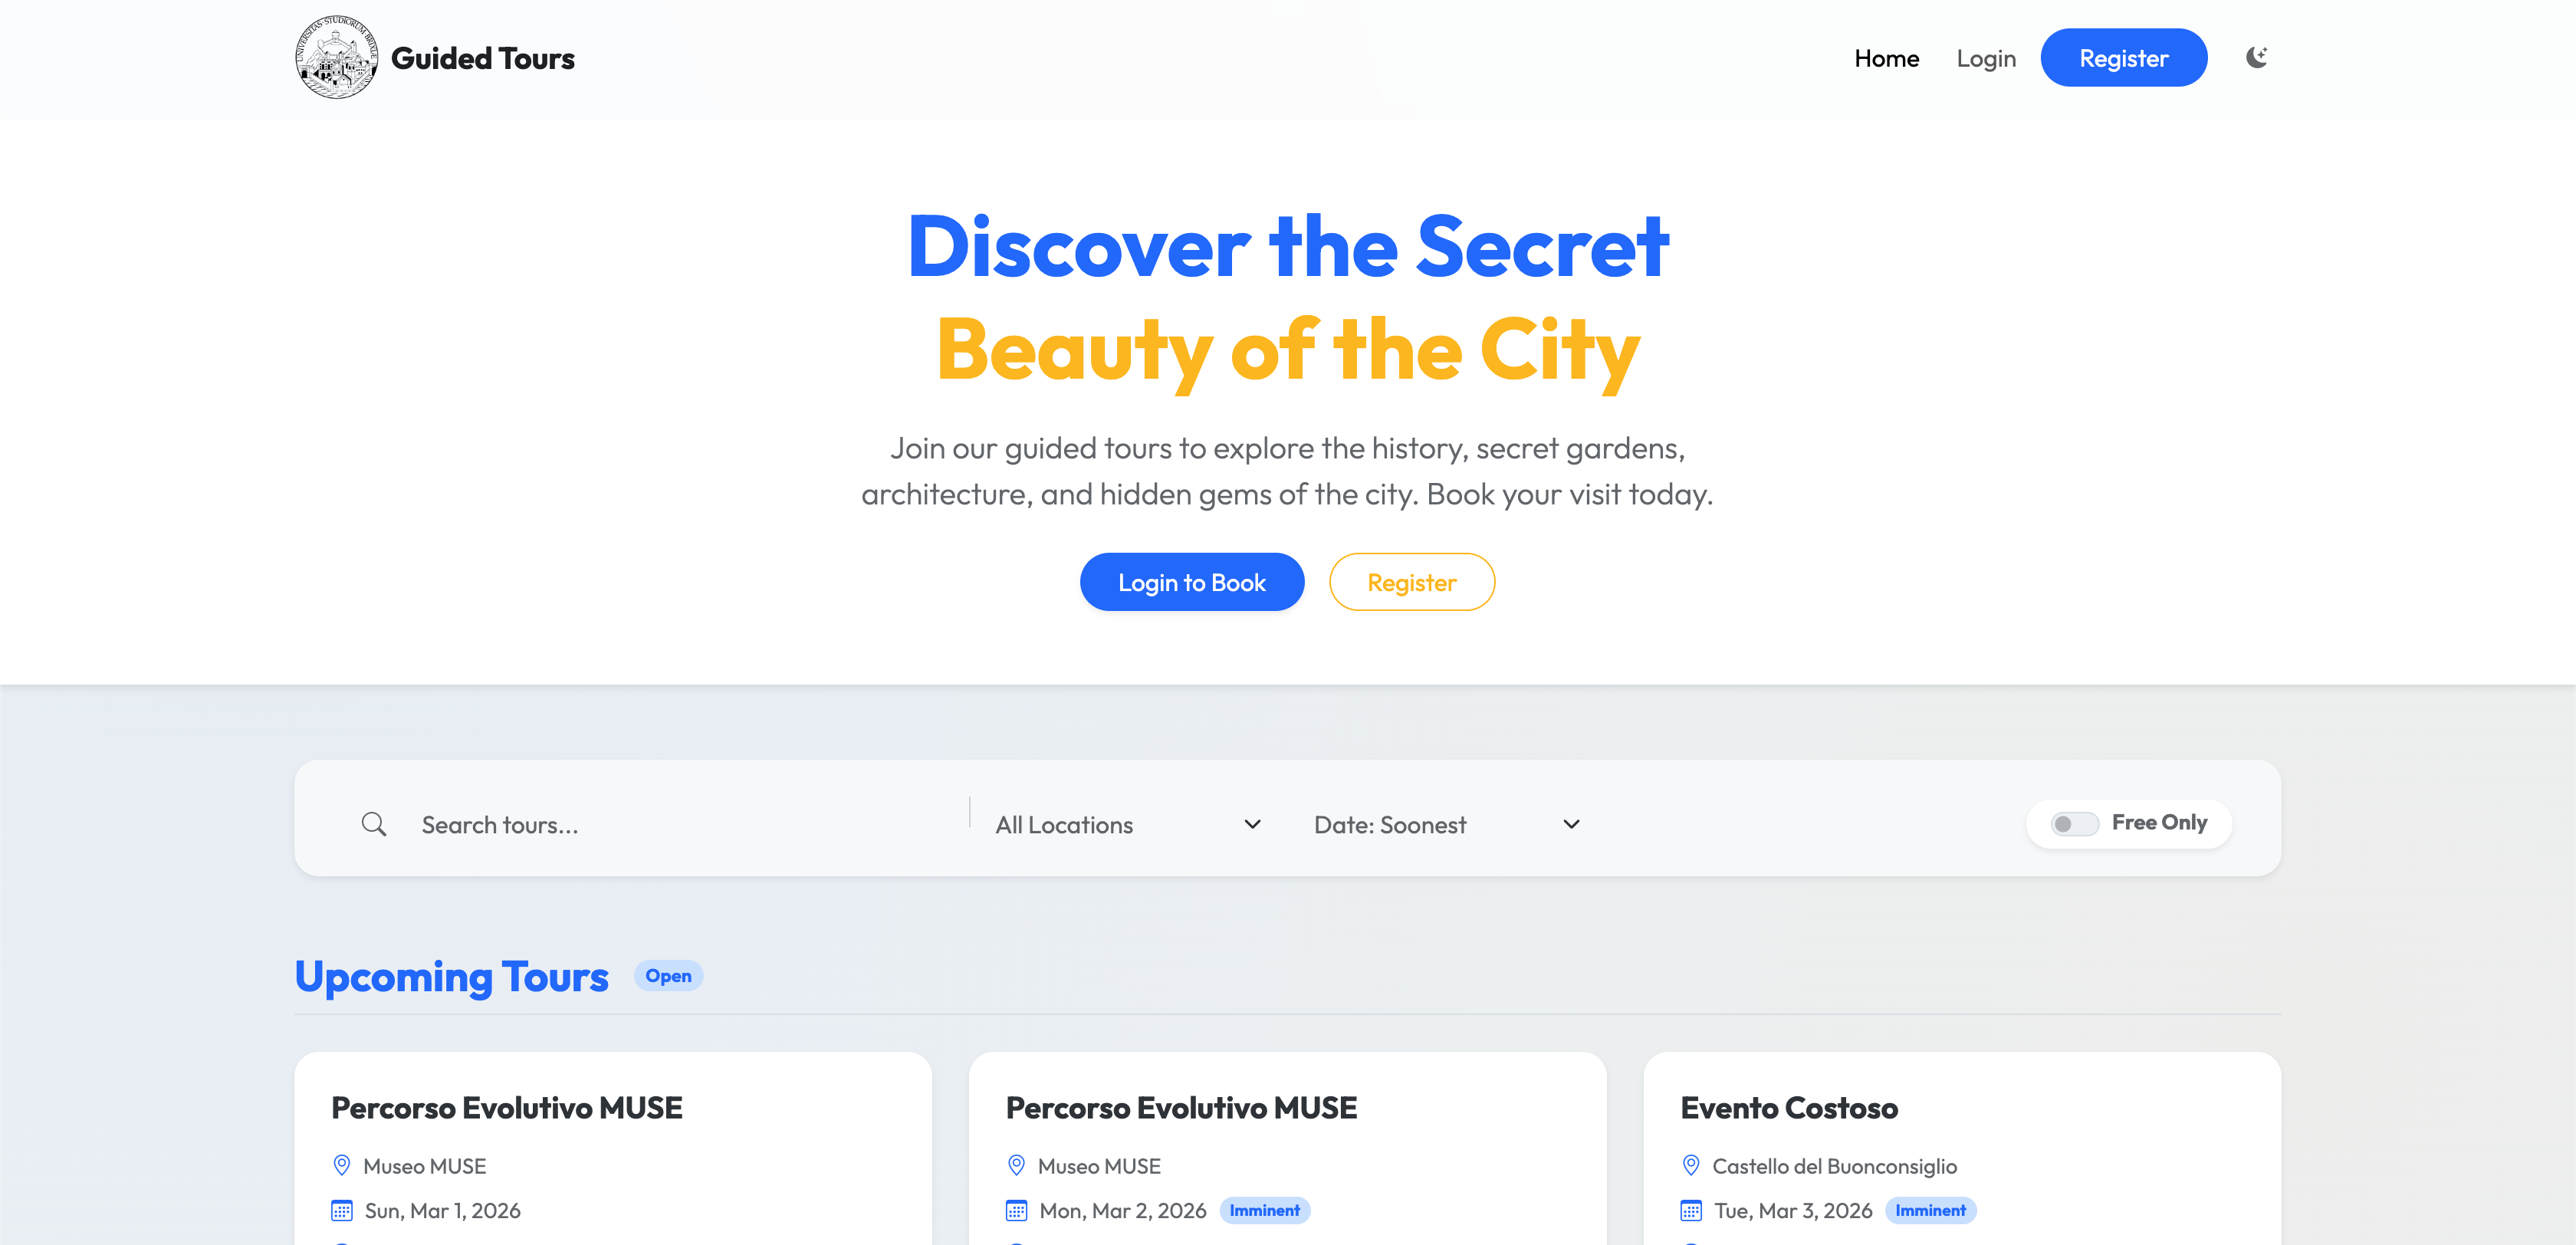
\includegraphics[width=0.9\textwidth, keepaspectratio]{capitoli/immagini/v2/v2_home.png}
    \caption{V2 -- Homepage in modalità ospite (utente non autenticato).}
    \label{fig:v2_home}
\end{figure}

\subsection{Autenticazione}

Le pagine di Login e Register nella V2 sono state semplificate e arricchite di meccanismi di supporto: toggle per la visibilità della password, validazione live dei campi e link diretto al recupero delle credenziali.

\begin{figure}[H]
    \centering
    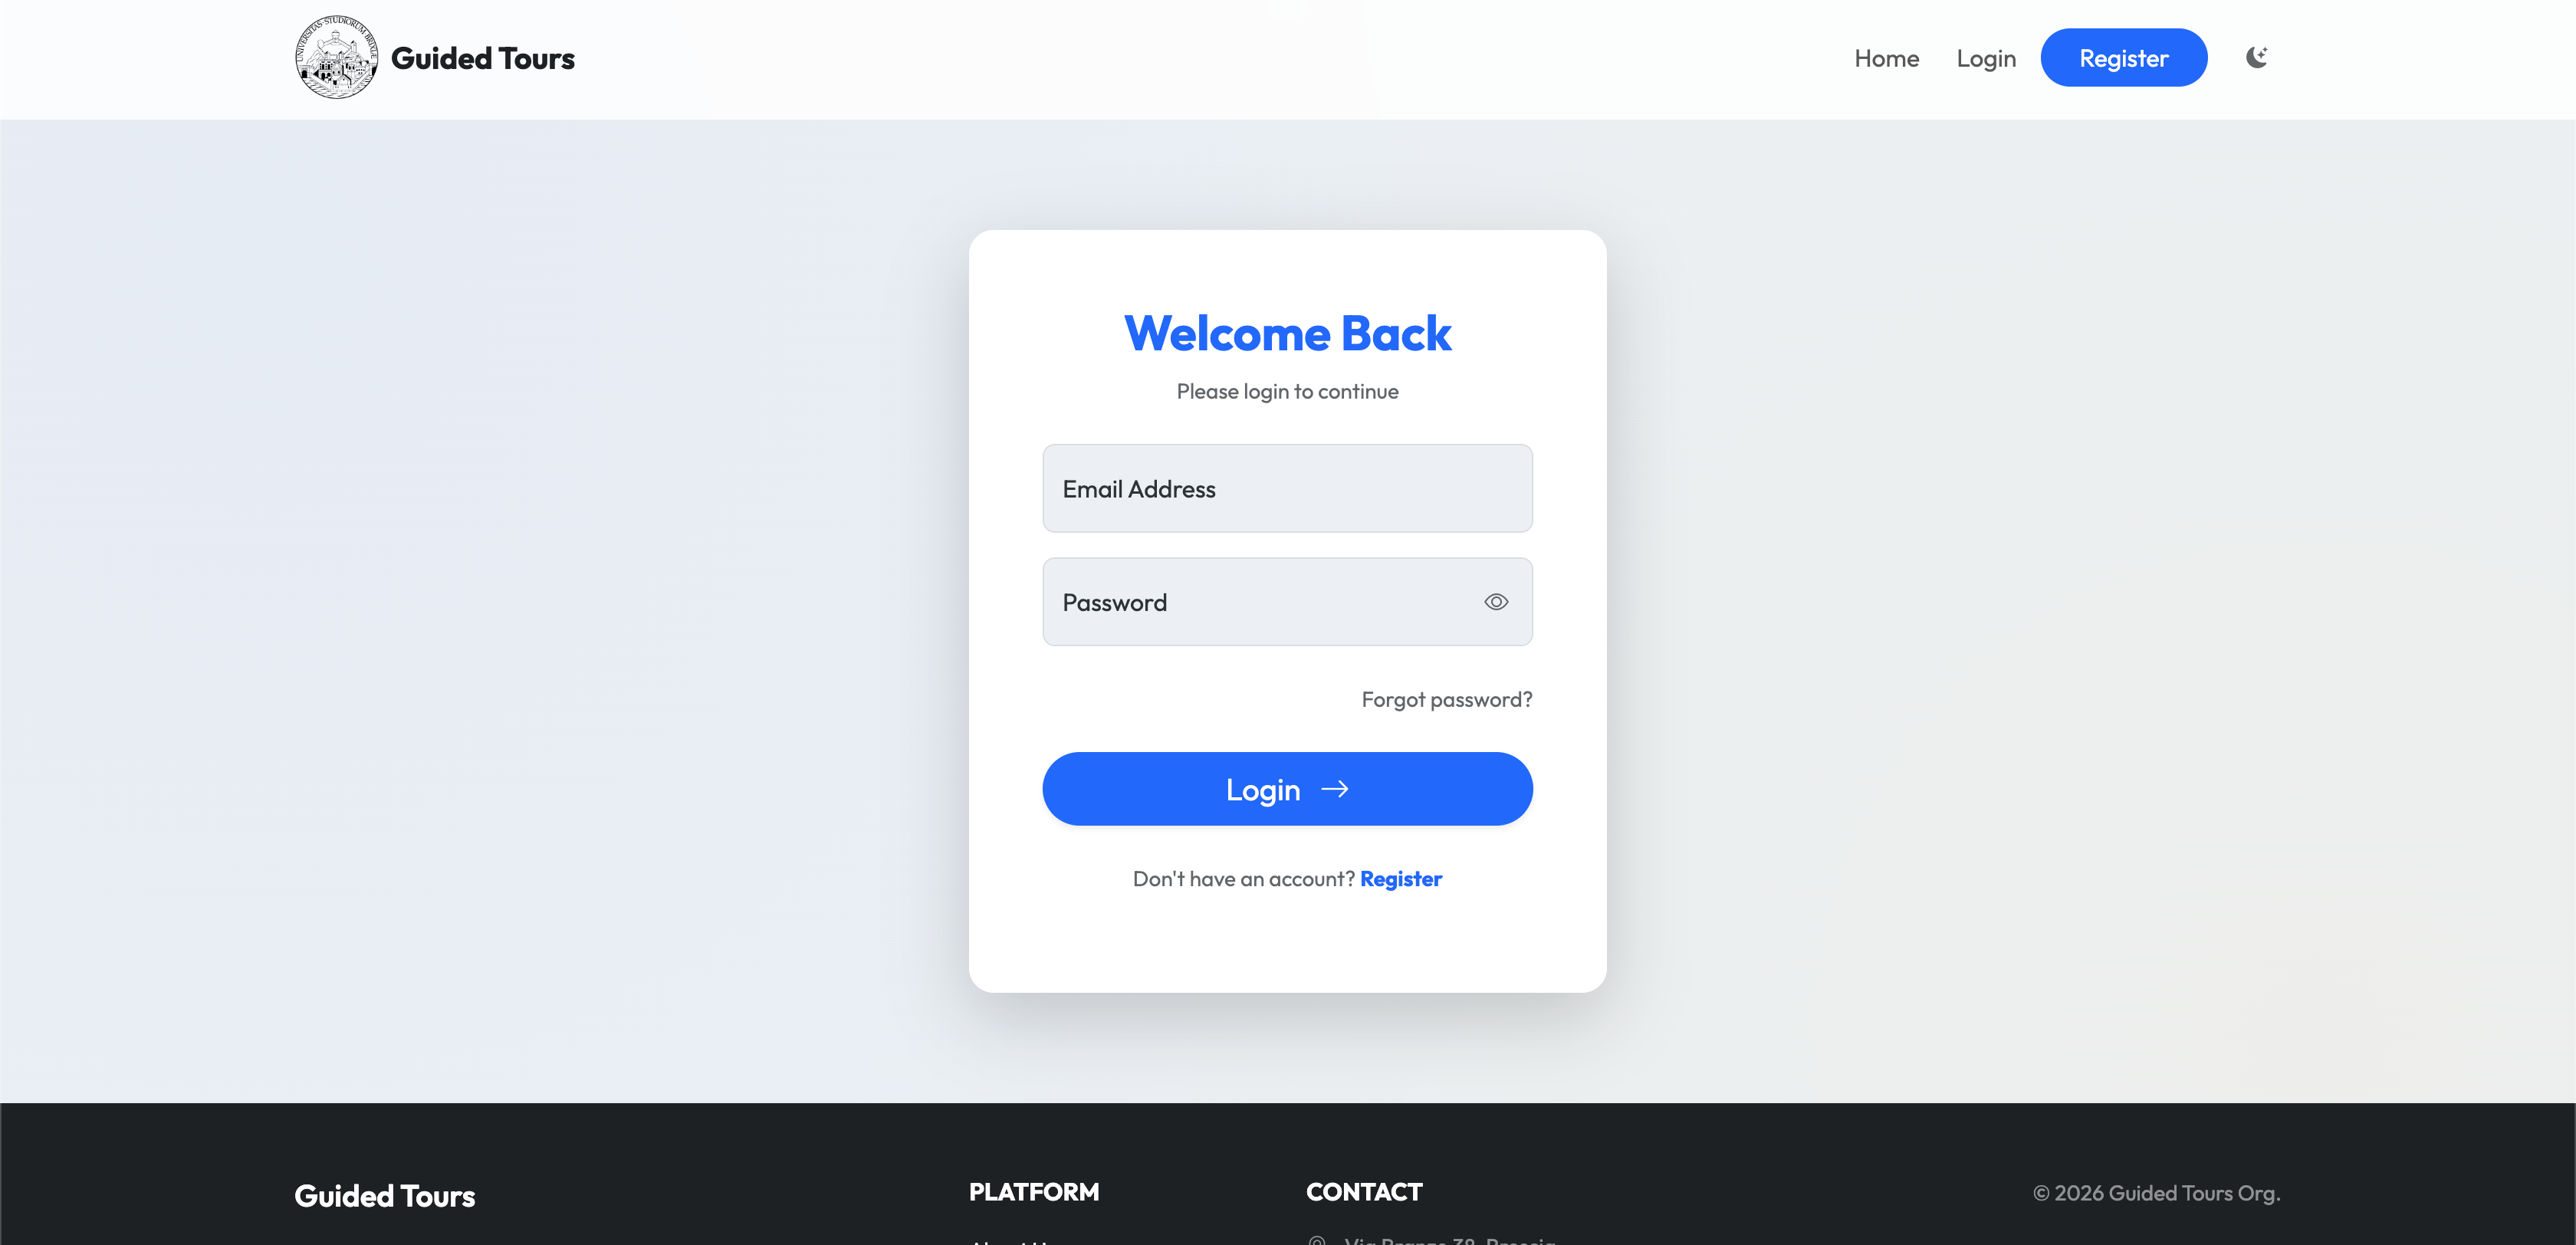
\includegraphics[width=0.9\textwidth, keepaspectratio]{capitoli/immagini/v2/v2_login.png}
    \caption{V2 -- Pagine di Autenticazione (Login e Register).}
    \label{fig:v2_auth}
\end{figure}

\subsection{Dashboard Fruitore}

La Dashboard del Customer nella V2 mostra le prenotazioni attive con il booking code in evidenza, la codifica cromatica semantica degli stati visita e il pulsante di cancellazione con modale di conferma.

\begin{figure}[H]
    \centering
    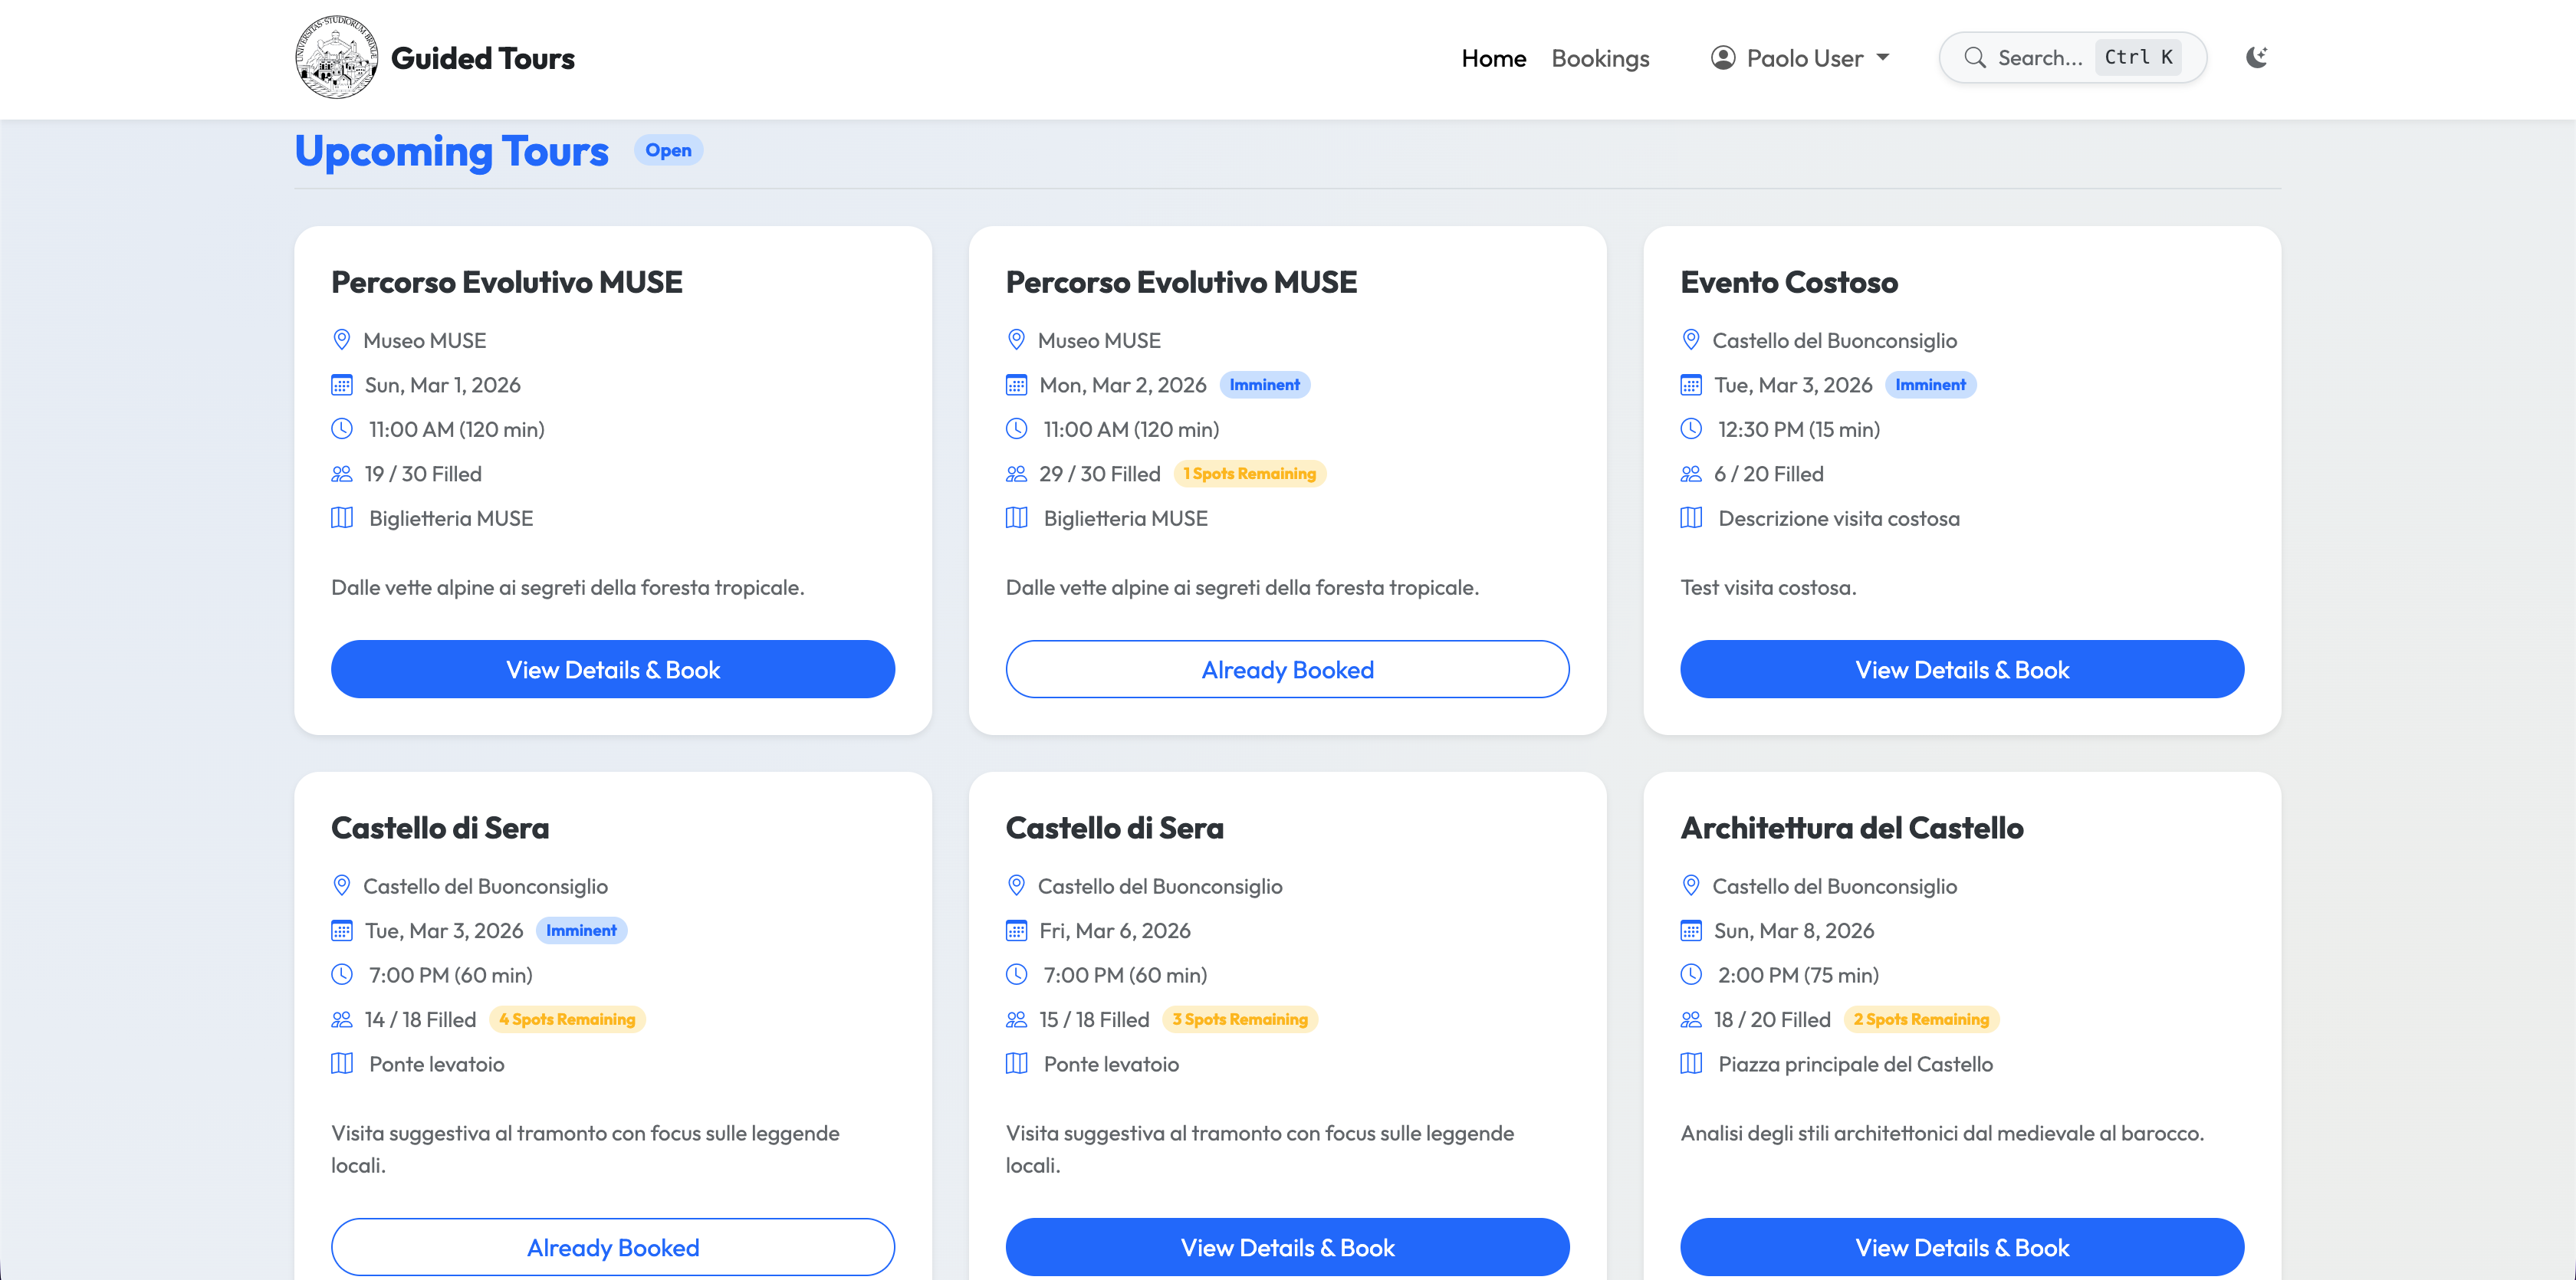
\includegraphics[width=0.9\textwidth, keepaspectratio]{capitoli/immagini/v2/v2_dashboard.png}
    \caption{V2 -- Dashboard Fruitore: prenotazioni attive con booking code, badge di stato e azioni disponibili.}
    \label{fig:v2_dashboard}
\end{figure}

\subsection{Area Amministratore}

Il pannello amministrativo comprende il configuratore a schede (Places, Visit Types, Users), il pannello di Visit Planning con raggruppamento mensile e il form di creazione visite con flusso guidato step-by-step.

\begin{figure}[H]
    \centering
    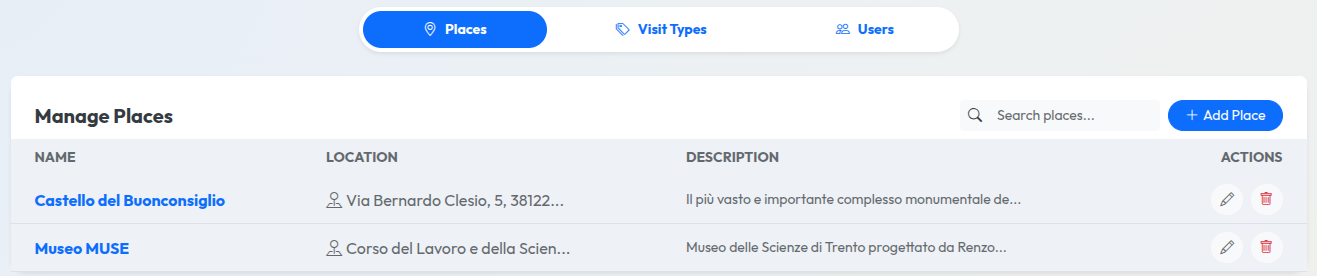
\includegraphics[width=0.9\textwidth, keepaspectratio]{capitoli/immagini/v2/v2_admin_conf.png}
    \caption{V2 -- Admin Configurator: pannello a schede per la gestione centralizzata delle entità del sistema.}
    \label{fig:v2_admin_conf}
\end{figure}

\begin{figure}[H]
    \centering
    \begin{subfigure}[b]{0.47\textwidth}
        \centering
        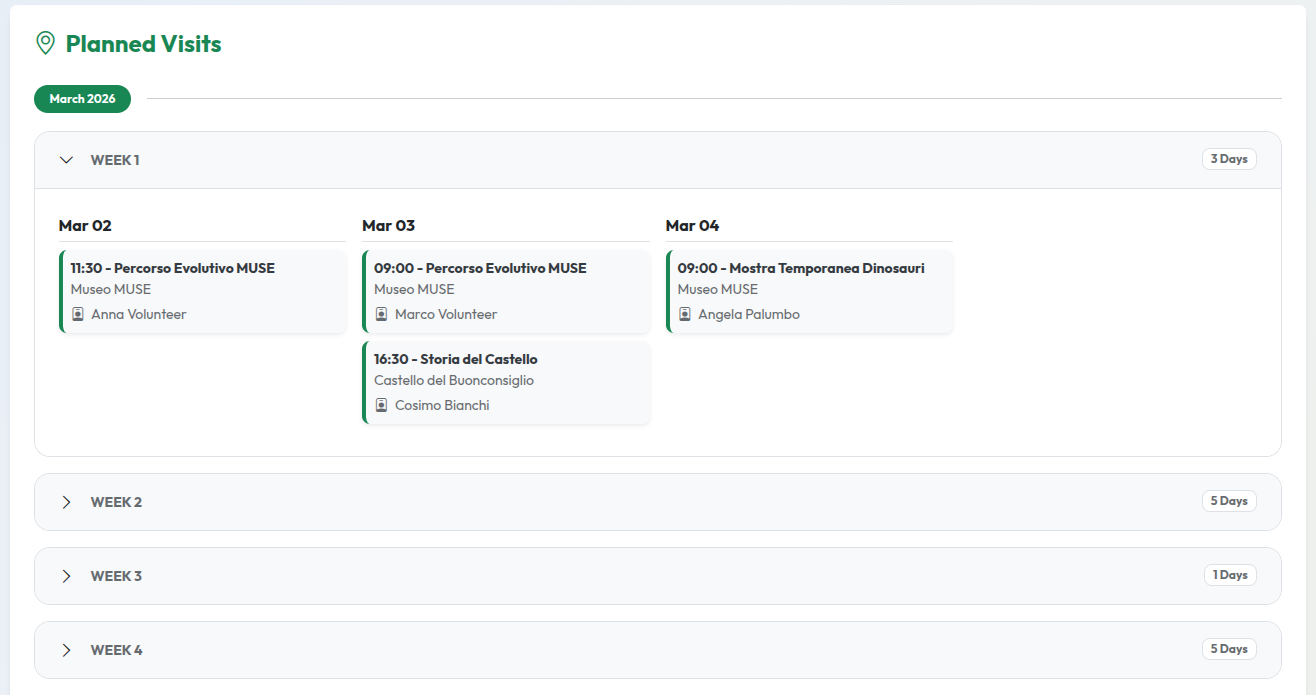
\includegraphics[width=\textwidth, keepaspectratio]{capitoli/immagini/v2/v2_add_visit.png}
        \caption{V1 (Prima)}
    \end{subfigure}
    \hfill
    \begin{subfigure}[b]{0.47\textwidth}
        \centering
        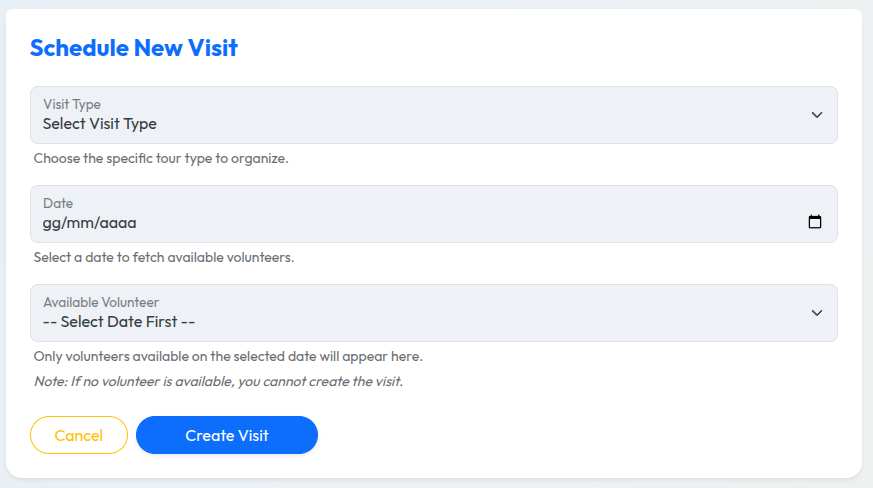
\includegraphics[width=\textwidth, keepaspectratio]{capitoli/immagini/v2/v2_admin_planning.png}
        \caption{V2 (Dopo)}
    \end{subfigure}
    \caption{V2 -- Visit Planning raggruppato per mese (sinistra) e form Add Visit con flusso guidato (destra).}
    \label{fig:v2_planning}
\end{figure}

\subsection{Area Volontario (Guida)}

L'area riservata alle Guide presenta la pagina delle visite assegnate con banner operativo e il calendario per la dichiarazione delle disponibilità mensili.

\begin{figure}[H]
    \centering
    \begin{subfigure}[b]{0.47\textwidth}
        \centering
        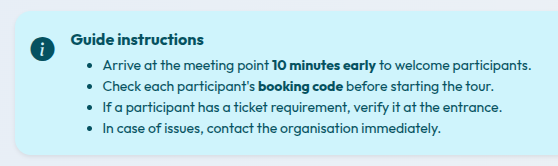
\includegraphics[width=\textwidth, keepaspectratio]{capitoli/immagini/v2/v2_guide_visits.png}
        \caption{V1 (Prima)}
    \end{subfigure}
    \hfill
    \begin{subfigure}[b]{0.47\textwidth}
        \centering
        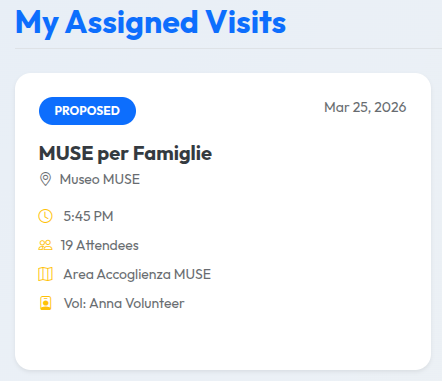
\includegraphics[width=\textwidth, keepaspectratio]{capitoli/immagini/v2/v2_guide_calendar.png}
        \caption{V2 (Dopo)}
    \end{subfigure}
    \caption{V2 -- "My Assigned Visits" con banner istruzioni operative (sinistra) e calendario disponibilità (destra).}
    \label{fig:v2_guide}
\end{figure}

% ─────────────────────────────────────────────────────────────────────────────
\newpage
\section{Riepilogo Interventi per Area}
\label{sec:riepilogo}

I paragrafi precedenti hanno descritto le soluzioni architetturali e i pattern adottati nella riprogettazione. In questa sezione viene fornita una mappatura diretta tra i singoli problemi identificati nel Capitolo 3 e gli interventi implementati, organizzata per area funzionale dell'applicativo.

\subsection{Homepage e Navigazione Globale}

\begin{table}[H]
\centering
\renewcommand{\arraystretch}{1.4}
\small
\begin{tabularx}{\textwidth}{|c|X|c|X|}
\hline
\textbf{P\#} & \textbf{Problema} & \textbf{Sev.} & \textbf{Soluzione adottata} \\ \hline
3  & Semantica colore "Proposed"        & 2 & Stato rinominato "Upcoming"; badge \texttt{bg-primary-subtle} (blu neutrale) in tutte le viste. \\ \hline
4  & Inconsistenza cromatica "Proposed" & 2 & Uso sistematico di \texttt{bg-primary-subtle}: eliminata la variante gialla. \\ \hline
5  & Chiarezza nota pagamento           & 2 & Prezzo esplicito su ogni card (\textit{Free} oppure \textit{€X}); rimosso l'avviso generico ambiguo. \\ \hline
6  & Stile nota pagamento               & 2 & Avviso riformulato come banner \texttt{alert-warning} con icona Bootstrap, ad alto contrasto. \\ \hline
7  & Ambiguità cromatica stati visita   & 1 & "Confirmed" → \texttt{bg-success}; "Complete" → \texttt{bg-secondary}: distinzione cromatica netta. \\ \hline
8  & Mancanza feedback disponibilità    & 1 & Aggiunto badge "Filling Fast" e contatore "X/Y Filled" su ogni card tour. \\ \hline
9  & Ridondanza "Visite confermate"     & 1 & Sezioni "Upcoming" e "Your Confirmed" mantenute distinte con intestazioni esplicite. \\ \hline
10 & Area cliccabile limitata           & 2 & Tutta la card è cliccabile tramite \texttt{stretched-link}; aggiunta classe \texttt{card-hover}. \\ \hline
11 & Gerarchia visiva debole            & 1 & Gerarchia tipografica \texttt{display-4} → \texttt{h3} → \texttt{h5} con Bootstrap; titoli in grassetto. \\ \hline
12 & Assenza shortcut area personale    & 1 & Bottone "My Dashboard" nell'hero section, visibile solo agli utenti autenticati. \\ \hline
—  & Mancanza personalizzazione Homepage & 1 & Sottotitolo hero personalizzato per ruolo: testo specifico per Guest, Customer, Guide e Admin. \\ \hline
\end{tabularx}
\caption{Interventi sulla Homepage e sulla navigazione globale.}
\label{tab:fix_home}
\end{table}

\begin{figure}[H]
    \centering
    \begin{subfigure}[b]{0.47\textwidth}
        \centering
        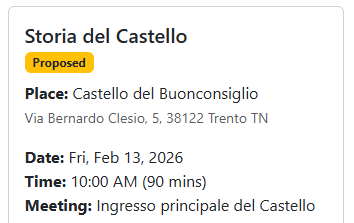
\includegraphics[width=\textwidth, keepaspectratio]{capitoli/immagini/p1.png}
        \caption{V1 (Prima)}
    \end{subfigure}
    \hfill
    \begin{subfigure}[b]{0.47\textwidth}
        \centering
        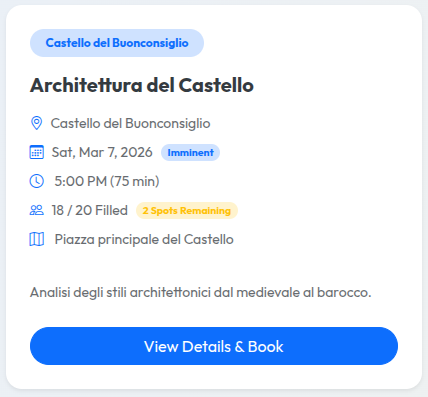
\includegraphics[width=\textwidth, keepaspectratio]{capitoli/immagini/v2/p3_v2.png}
        \caption{V2 (Dopo)}
    \end{subfigure}
    \caption{Fix P.3 -- Semantica colore stato visita: V1 a sinistra (badge giallo "Proposed"), V2 a destra (badge blu neutrale "Upcoming").}
    \label{fig:fix_p3}
\end{figure}

\begin{figure}[H]
    \centering
    \begin{subfigure}[b]{0.47\textwidth}
        \centering
        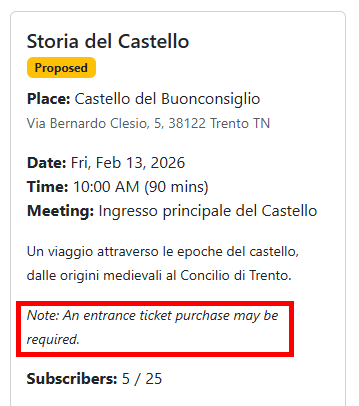
\includegraphics[width=\textwidth, keepaspectratio]{capitoli/immagini/p3.png}
        \caption{V1 (Prima)}
    \end{subfigure}
    \hfill
    \begin{subfigure}[b]{0.47\textwidth}
        \centering
        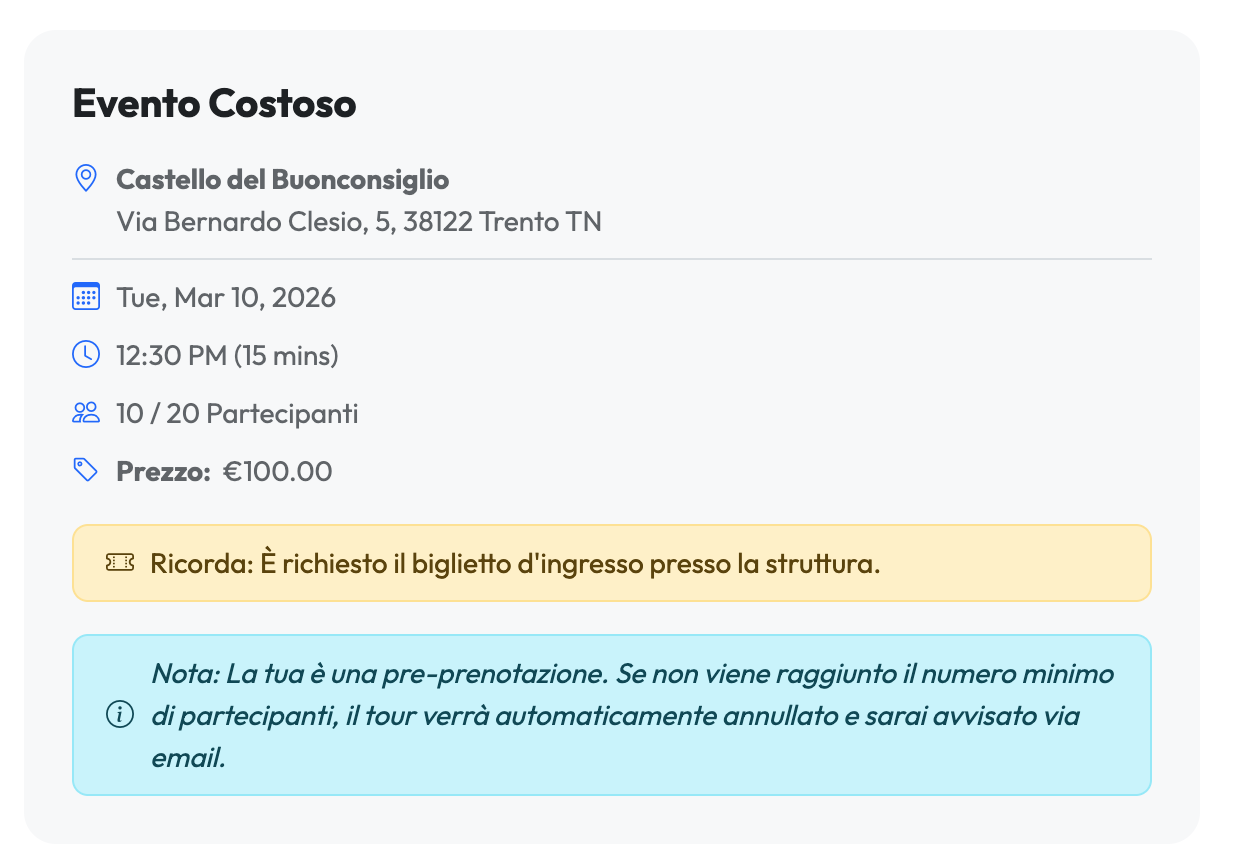
\includegraphics[width=\textwidth, keepaspectratio]{capitoli/immagini/v2/p6_v2.png}
        \caption{V2 (Dopo)}
    \end{subfigure}
    \caption{Fix P.6 -- Nota pagamento: V1 a sinistra (testo generico poco visibile), V2 a destra (banner \texttt{alert-warning} con icona).}
    \label{fig:fix_p6}
\end{figure}

\subsection{Footer e Navbar}

\begin{table}[H]
\centering
\renewcommand{\arraystretch}{1.4}
\small
\begin{tabularx}{\textwidth}{|c|X|c|X|}
\hline
\textbf{P\#} & \textbf{Problema} & \textbf{Sev.} & \textbf{Soluzione adottata} \\ \hline
13 & Incoerenza linguistica  & 1 & Footer interamente riscritto in inglese; rimossa la dicitura italiana "Sito di visite guidate". \\ \hline
35 & Email non cliccabili    & 2 & Tutti gli indirizzi email nel footer avvolti da tag \texttt{<a href="mailto:...">}. \\ \hline
\end{tabularx}
\caption{Interventi su Footer e Navbar.}
\label{tab:fix_footer}
\end{table}

\subsection{Autenticazione (Login e Register)}

\begin{table}[H]
\centering
\renewcommand{\arraystretch}{1.4}
\small
\begin{tabularx}{\textwidth}{|c|X|c|X|}
\hline
\textbf{P\#} & \textbf{Problema} & \textbf{Sev.} & \textbf{Soluzione adottata} \\ \hline
15 & Mancanza toggle visibilità password  & 1 & Icona occhio (Bootstrap Icons) con script JS \texttt{showPassword()} nelle pagine Login e Register. \\ \hline
16 & Navigazione ambigua verso Register   & 1 & Rimossi accessi multipli; unico link "Create an Account" nel footer della card di login. \\ \hline
17 & Ridondanza informativa Ruoli (Login) & 1 & Testo ridondante rimosso; sostituito con l'essenziale "Please login to continue". \\ \hline
18 & Feedback errore non user-friendly    & 1 & Messaggi di errore riformulati e presentati tramite Toast Notifications, chiari e non tecnici. \\ \hline
19 & Assenza recupero password            & 3 & Implementata pagina "Forgot Password" con reset tramite link inviato via email (\texttt{PasswordResetController}). \\ \hline
20 & Carico cognitivo posti disponibili   & 2 & Label esplicita "(X spots remaining)" accanto al campo numero partecipanti nel form di prenotazione. \\ \hline
21 & Navigazione ridondante verso Login   & 1 & Unico link "Already have an account? Login" nella pagina di registrazione. \\ \hline
22 & Ridondanza informativa Ruoli (Register) & 1 & Rimossa spiegazione dei ruoli; form di registrazione semplificato. \\ \hline
23 & Validazione tardiva input            & 2 & Aggiunta validazione JavaScript live: controllo lunghezza e corrispondenza password in tempo reale. \\ \hline
\end{tabularx}
\caption{Interventi sull'autenticazione.}
\label{tab:fix_auth}
\end{table}

\begin{figure}[H]
    \centering
    \begin{subfigure}[b]{0.47\textwidth}
        \centering
        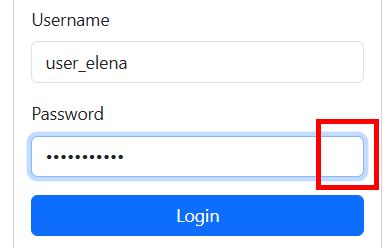
\includegraphics[width=\textwidth, keepaspectratio]{capitoli/immagini/p11.png}
        \caption{V1 (Prima)}
    \end{subfigure}
    \hfill
    \begin{subfigure}[b]{0.47\textwidth}
        \centering
        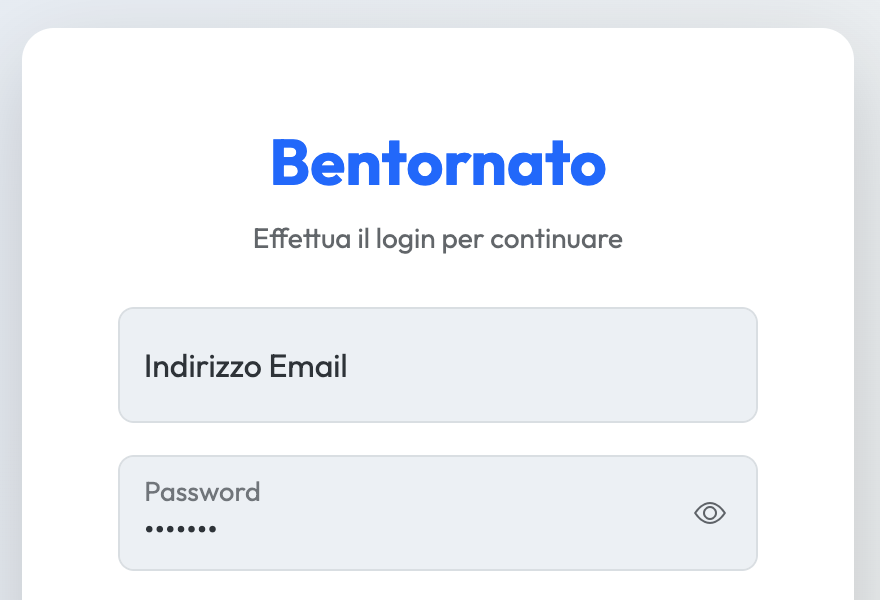
\includegraphics[width=\textwidth, keepaspectratio]{capitoli/immagini/v2/p15_v2.png}
        \caption{V2 (Dopo)}
    \end{subfigure}
    \caption{Fix P.15 -- Toggle visibilità password: V1 a sinistra (campo senza icona), V2 a destra (icona occhio per mostrare/nascondere la password).}
    \label{fig:fix_p15}
\end{figure}

\begin{figure}[H]
    \centering
    \begin{subfigure}[b]{0.47\textwidth}
        \centering
        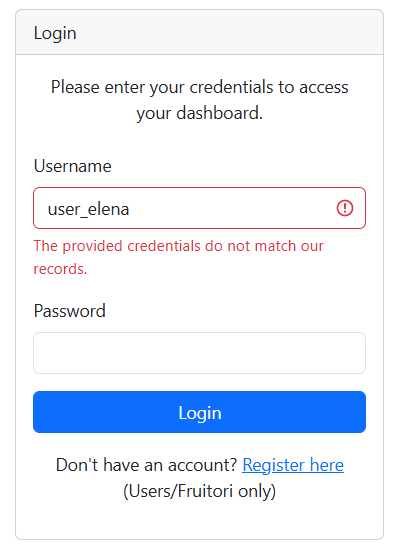
\includegraphics[width=\textwidth, keepaspectratio]{capitoli/immagini/p17.png}
        \caption{V1 (Prima)}
    \end{subfigure}
    \hfill
    \begin{subfigure}[b]{0.47\textwidth}
        \centering
        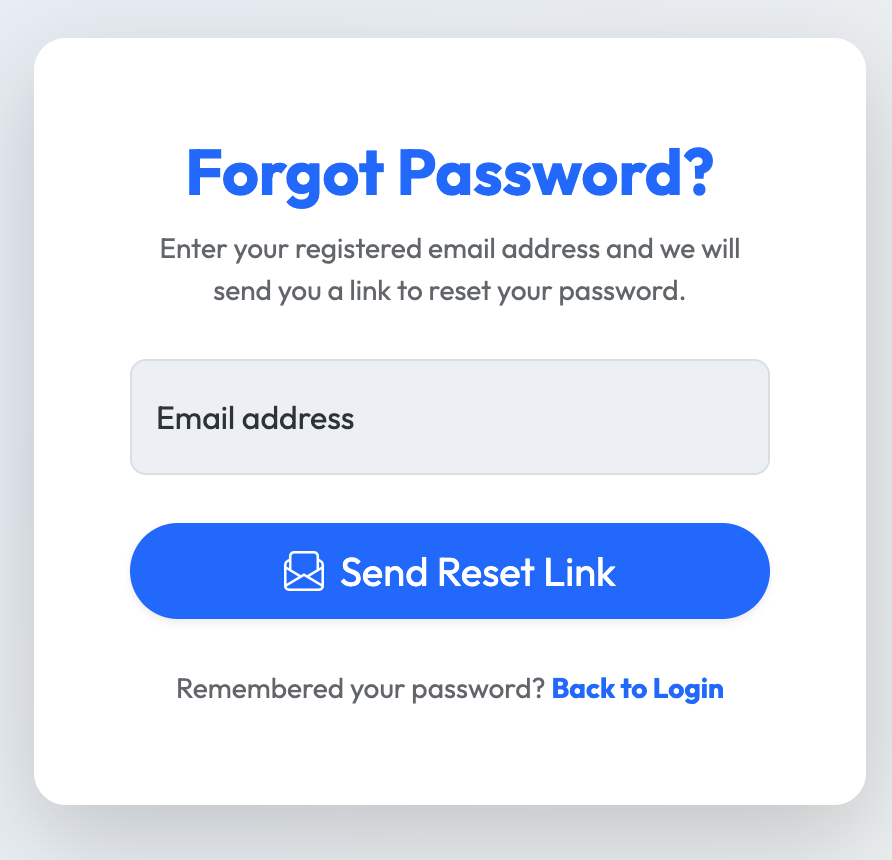
\includegraphics[width=\textwidth, keepaspectratio]{capitoli/immagini/v2/p19_v2.png}
        \caption{V2 (Dopo)}
    \end{subfigure}
    \caption{Fix P.19 -- Recupero password: V1 a sinistra (nessun link di recupero), V2 a destra (pagina "Forgot Password" dedicata).}
    \label{fig:fix_p19}
\end{figure}

\begin{figure}[H]
    \centering
    \begin{subfigure}[b]{0.47\textwidth}
        \centering
        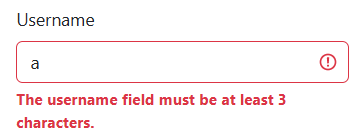
\includegraphics[width=\textwidth, keepaspectratio]{capitoli/immagini/p21.png}
        \caption{V1 (Prima)}
    \end{subfigure}
    \hfill
    \begin{subfigure}[b]{0.47\textwidth}
        \centering
        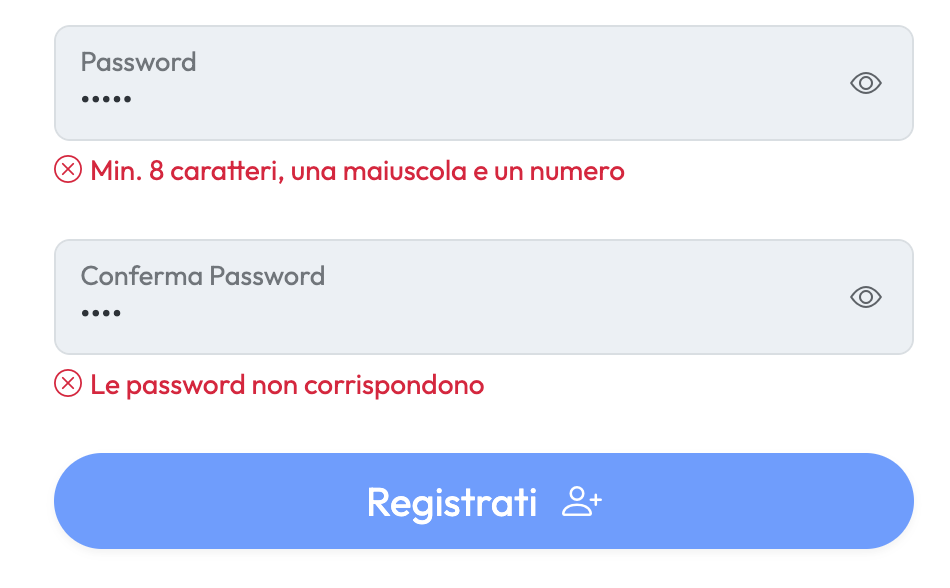
\includegraphics[width=\textwidth, keepaspectratio]{capitoli/immagini/v2/p23_v2.png}
        \caption{V2 (Dopo)}
    \end{subfigure}
    \caption{Fix P.23 -- Validazione live password: V1 a sinistra (nessun feedback), V2 a destra (indicatori in tempo reale su lunghezza e corrispondenza).}
    \label{fig:fix_p23}
\end{figure}

\subsection{Dashboard Fruitore}

\begin{table}[H]
\centering
\renewcommand{\arraystretch}{1.4}
\small
\begin{tabularx}{\textwidth}{|c|X|c|X|}
\hline
\textbf{P\#} & \textbf{Problema} & \textbf{Sev.} & \textbf{Soluzione adottata} \\ \hline
24 & Visibilità "Booking code"            & 1 & Codice visualizzato in font monospaziato bold con etichetta "Booking Code" esplicita. \\ \hline
25 & Ambiguità etichetta "Participant"    & 2 & Etichetta standardizzata "X Participants" coerente con il resto dell'interfaccia. \\ \hline
26 & Affordance ingannevole "My Booking" & 2 & Rimosso il menu a tendina ambiguo; sostituito con bottone esplicito \texttt{btn-danger} "Cancel Booking". \\ \hline
27 & Stile pulsante eliminazione          & 1 & Pulsante in stile \texttt{btn-danger} e testo rosso, coerente con il Design System. \\ \hline
\end{tabularx}
\caption{Interventi sulla Dashboard Fruitore.}
\label{tab:fix_dashboard}
\end{table}

\begin{figure}[H]
    \centering
    \begin{subfigure}[b]{0.47\textwidth}
        \centering
        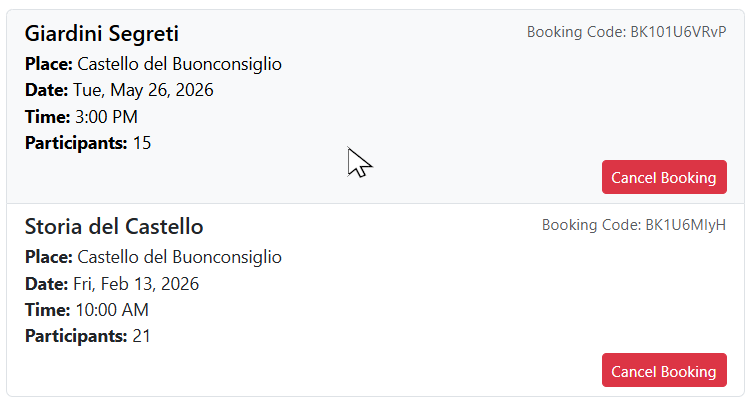
\includegraphics[width=\textwidth, keepaspectratio]{capitoli/immagini/p24.png}
        \caption{V1 (Prima)}
    \end{subfigure}
    \hfill
    \begin{subfigure}[b]{0.40\textwidth}
        \centering
        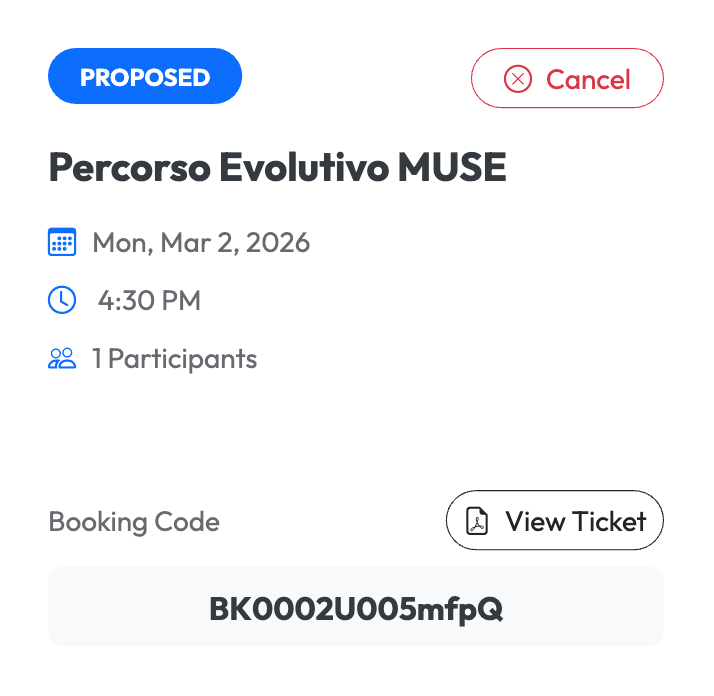
\includegraphics[width=\textwidth, keepaspectratio]{capitoli/immagini/v2/p26_v2.png}
        \caption{V2 (Dopo)}
    \end{subfigure}
    \caption{Fix P.26 -- Affordance "My Booking": V1 a sinistra, V2 a destra (bottone meno impattante "Cancel Booking" con modale di conferma).}
    \label{fig:fix_p26}
\end{figure}

\subsection{Area Amministratore}

\begin{table}[H]
\centering
\renewcommand{\arraystretch}{1.4}
\small
\begin{tabularx}{\textwidth}{|c|X|c|X|}
\hline
\textbf{P\#} & \textbf{Problema} & \textbf{Sev.} & \textbf{Soluzione adottata} \\ \hline
28 & Inconsistenza terminologica            & 1 & "Tours" e "Bookings" lato utente; "Visits" riservato al contesto amministrativo (dominio tecnico corretto). \\ \hline
29 & Incoerenza spaziatura Header           & 1 & Navbar Bootstrap standard con padding uniformi in tutte le pagine. \\ \hline
30 & Validazione tardiva aggiunta utente    & 2 & Validazione JS real-time per la password nel modale di creazione utente (\texttt{admin/configurator}). \\ \hline
31 & Assenza conferma eliminazione          & 4 & Global Delete Confirmation Modal: pop-up obbligatorio con avviso "This action cannot be undone" prima di ogni eliminazione. \\ \hline
32 & Disorganizzazione layout Visit Planning & 1 & Layout a card raggruppate per mese nel pannello \texttt{visit-planning.blade.php}. \\ \hline
33 & Flusso inserimento non intuitivo       & 3 & Flusso guidato in sequenza: selezione Tipo Visita → Data → Volontario disponibile (\texttt{admin/visits/create}). \\ \hline
34 & Mancanza feedback su vincoli           & 3 & Help text espliciti accanto ad ogni campo critico (data minima, assenza volontari disponibili). \\ \hline
40 & Colore bottone non coerente            & 2 & Bottone "Change Password" nel profilo allineato al Design System: rimosso lo stile rosso fuorviante. \\ \hline
\end{tabularx}
\caption{Interventi sull'Area Amministratore.}
\label{tab:fix_admin}
\end{table}

\begin{figure}[H]
    \centering
    \begin{subfigure}[b]{0.47\textwidth}
        \centering
        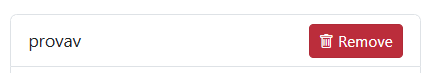
\includegraphics[width=\textwidth, keepaspectratio]{capitoli/immagini/p29.png}
        \caption{V1 (Prima)}
    \end{subfigure}
    \hfill
    \begin{subfigure}[b]{0.47\textwidth}
        \centering
        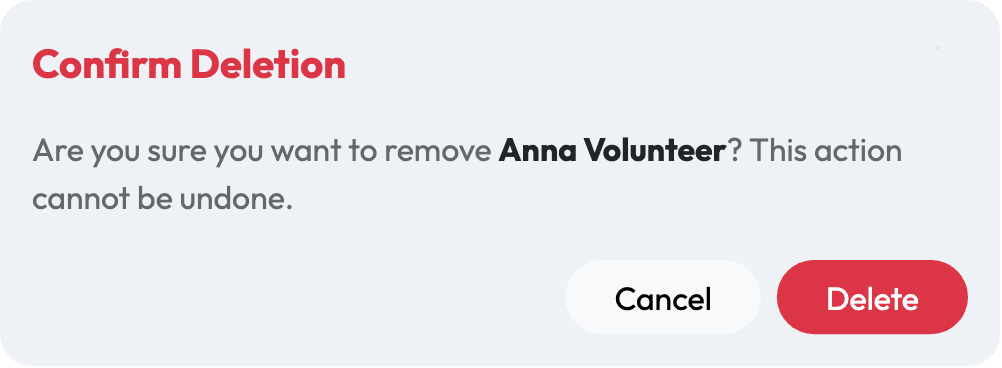
\includegraphics[width=\textwidth, keepaspectratio]{capitoli/immagini/v2/p31_v2.png}
        \caption{V2 (Dopo)}
    \end{subfigure}
    \caption{Fix P.31 -- Conferma eliminazione: V1 a sinistra (eliminazione immediata senza dialogo), V2 a destra (Global Delete Confirmation Modal con avviso "This action cannot be undone").}
    \label{fig:fix_p31}
\end{figure}

\begin{figure}[H]
    \centering
    \begin{subfigure}[b]{0.47\textwidth}
        \centering
        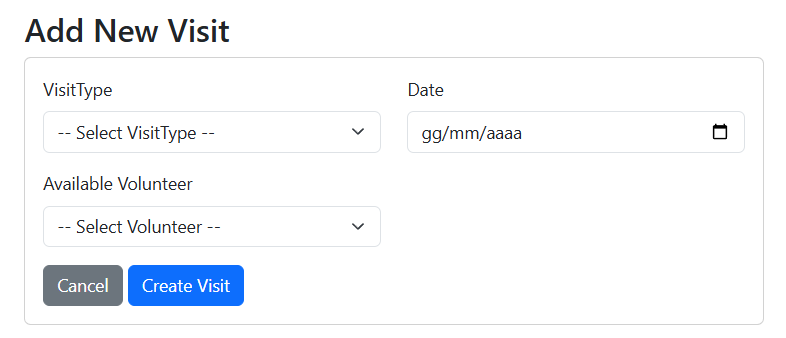
\includegraphics[width=\textwidth, keepaspectratio]{capitoli/immagini/p31.png}
        \caption{V1 (Prima)}
    \end{subfigure}
    \hfill
    \begin{subfigure}[b]{0.47\textwidth}
        \centering
        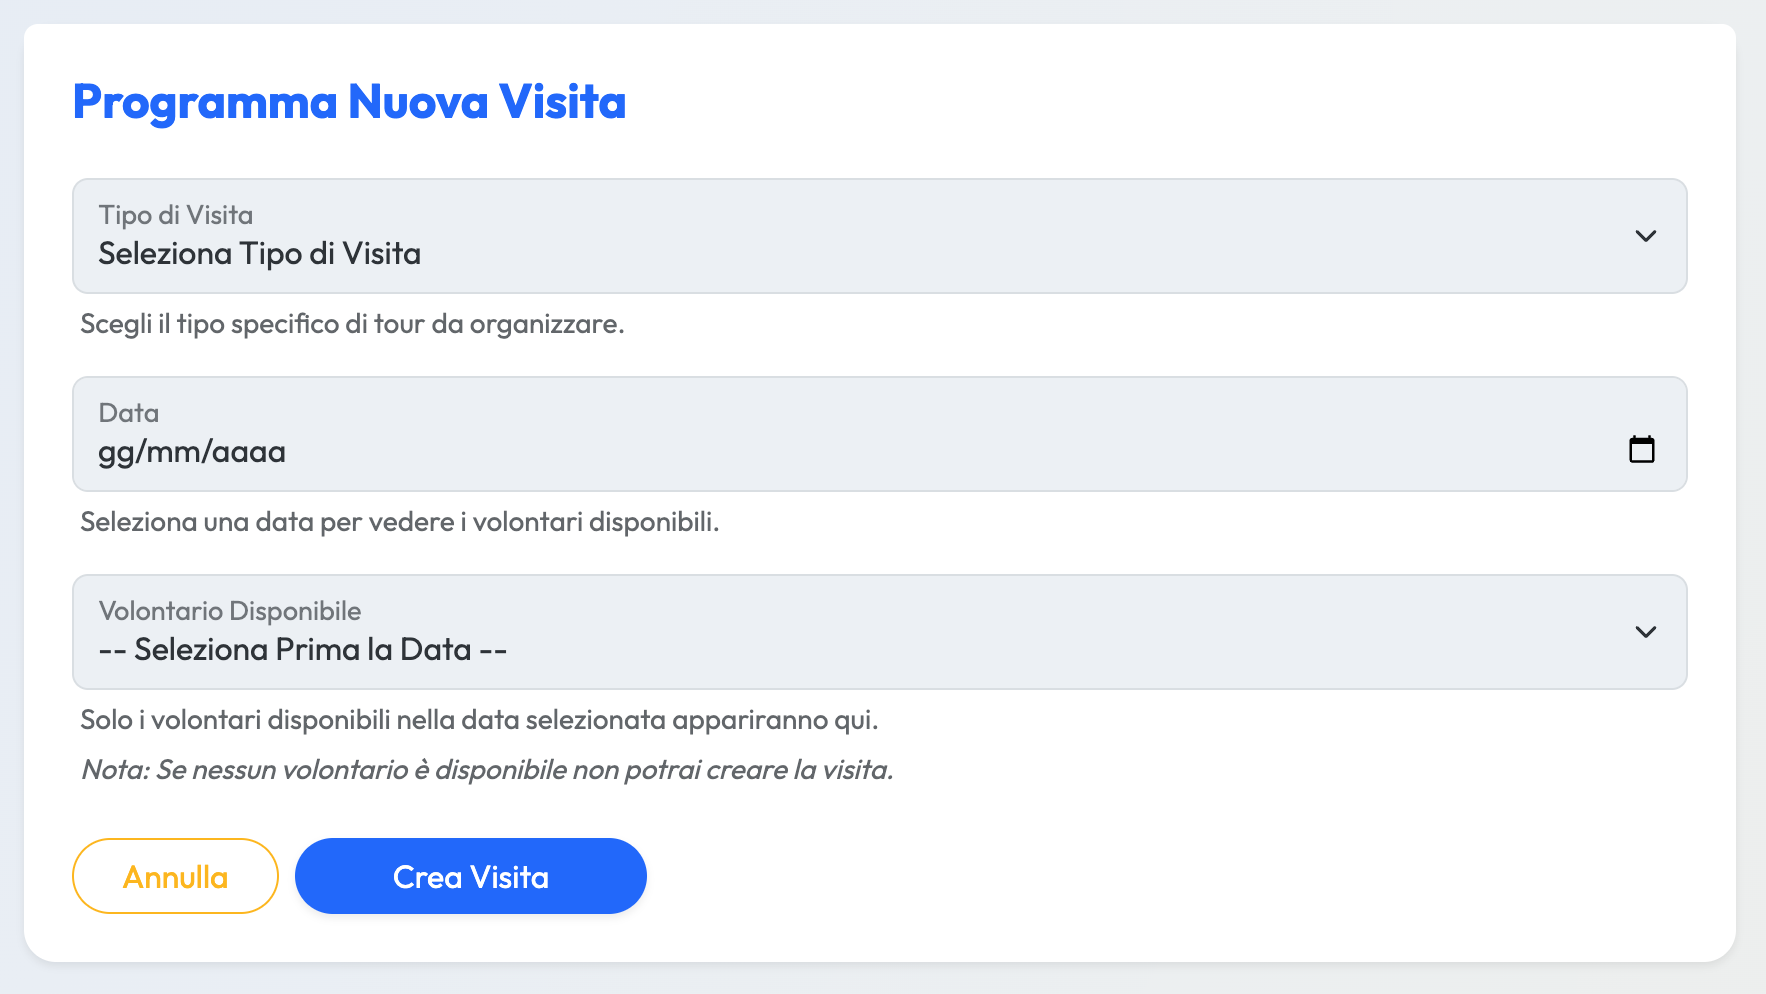
\includegraphics[width=\textwidth, keepaspectratio]{capitoli/immagini/v2/p33_v2.png}
        \caption{V2 (Dopo)}
    \end{subfigure}
    \caption{Fix P.33 -- Flusso inserimento visita: V1 a sinistra (form non guidato), V2 a destra (flusso step-by-step Tipo → Data → Volontario disponibile).}
    \label{fig:fix_p33}
\end{figure}

\subsection{Area Volontario (Guida)}

\begin{table}[H]
\centering
\renewcommand{\arraystretch}{1.4}
\small
\begin{tabularx}{\textwidth}{|c|X|c|X|}
\hline
\textbf{P\#} & \textbf{Problema} & \textbf{Sev.} & \textbf{Soluzione adottata} \\ \hline
37 & Assenza indicazioni operative           & 2 & Banner \texttt{alert-info} con istruzioni operative (puntualità, verifica booking code, gestione imprevisti) nella pagina "My Assigned Visits". \\ \hline
38 & Ridondanza nome volontario nelle card   & 1 & Il nome del volontario assegnato viene nascosto se corrisponde all'utente loggato; visibile solo agli altri ruoli. \\ \hline
\end{tabularx}
\caption{Interventi sull'Area Volontario.}
\label{tab:fix_volontario}
\end{table}

\begin{figure}[H]
    \centering
    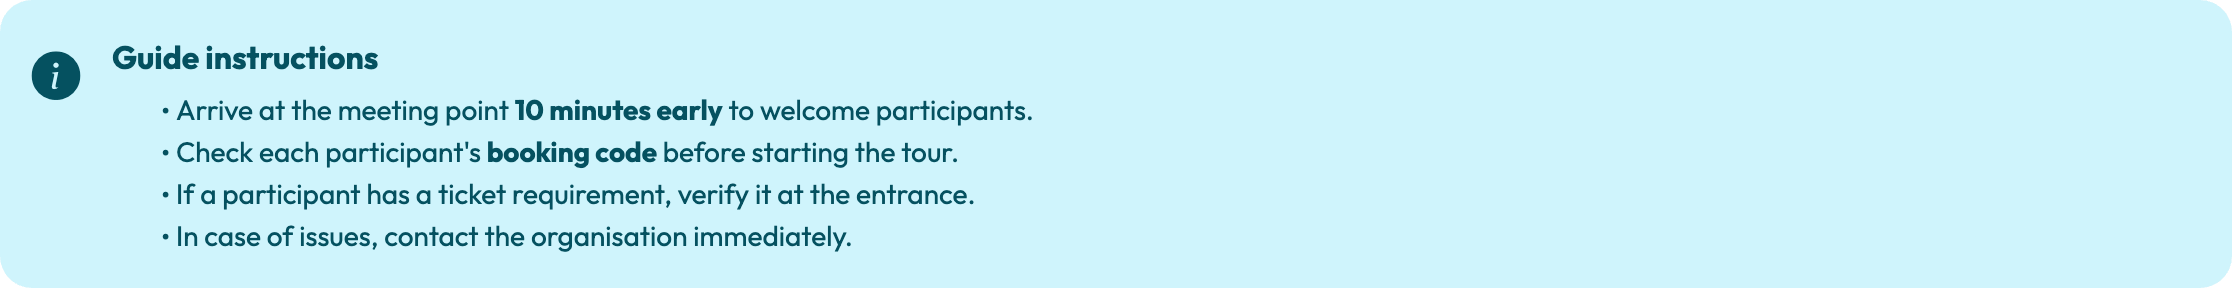
\includegraphics[width=0.85\textwidth, keepaspectratio]{capitoli/immagini/v2/p37_v2.png}
    \caption{Fix P.37 -- Banner istruzioni operative nella pagina "My Assigned Visits": avviso contestuale con promemoria su puntualità, verifica booking code e gestione imprevisti.}
    \label{fig:fix_p37}
\end{figure}

% ─────────────────────────────────────────────────────────────────────────────
\newpage
\section{Dettaglio Risoluzione Problemi}
\label{sec:dettaglio}

Di seguito viene presentata una descrizione dettagliata, corredata da confronti visivi prima/dopo, per ogni problema di usabilità risolto nella versione riprogettata. I problemi sono organizzati per area funzionale, in accordo con la struttura del Capitolo 3.

\subsection{Homepage e Navigazione Globale}

\noindent\textbf{P.3 -- Semantica colore "Proposed"} \hfill \textit{Severità: 2}

Nella versione originale lo stato "Proposed" era codificato in giallo, colore semanticamente associato a un avviso (\textit{warning}), creando ambiguità sulla natura del badge. In V2 lo stato è rinominato "Upcoming" e adotta \texttt{bg-primary-subtle} (blu), neutro e semanticamente corretto.

\begin{figure}[H]
    \centering
    \begin{subfigure}[b]{0.47\textwidth}
        \centering
        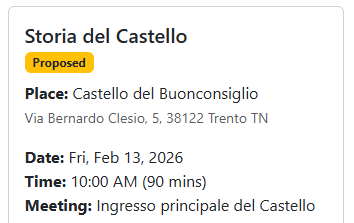
\includegraphics[width=\textwidth, keepaspectratio]{capitoli/immagini/p1.png}
        \caption{V1 (Prima)}
    \end{subfigure}
    \hfill
    \begin{subfigure}[b]{0.47\textwidth}
        \centering
        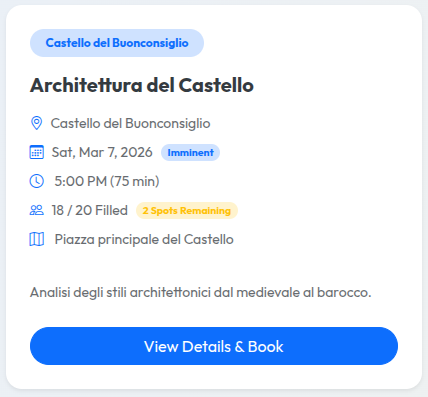
\includegraphics[width=\textwidth, keepaspectratio]{capitoli/immagini/v2/p3_v2.png}
        \caption{V2 (Dopo)}
    \end{subfigure}
    \caption{P.3 -- Badge stato: V1 (badge giallo "Proposed") vs V2 (badge blu "Upcoming").}
    \label{fig:det_p3}
\end{figure}

\noindent\textbf{P.4 -- Inconsistenza cromatica "Proposed"} \hfill \textit{Severità: 2}

Lo stesso stato compariva giallo in alcune viste e blu in altre. In V2 \texttt{bg-primary-subtle} è adottato uniformemente in tutte le schermate dell'applicativo.

\begin{figure}[H]
    \centering
    \begin{subfigure}[b]{0.47\textwidth}
        \centering
        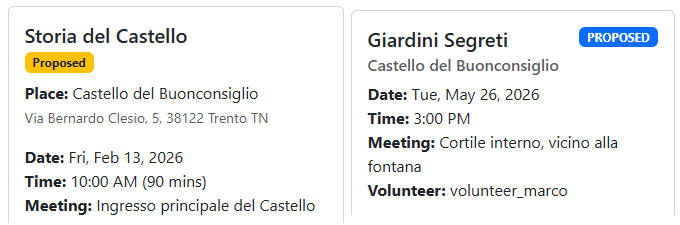
\includegraphics[width=\textwidth, keepaspectratio]{capitoli/immagini/p2.png}
        \caption{V1 (Prima)}
    \end{subfigure}
    \hfill
    \begin{subfigure}[b]{0.47\textwidth}
        \centering
        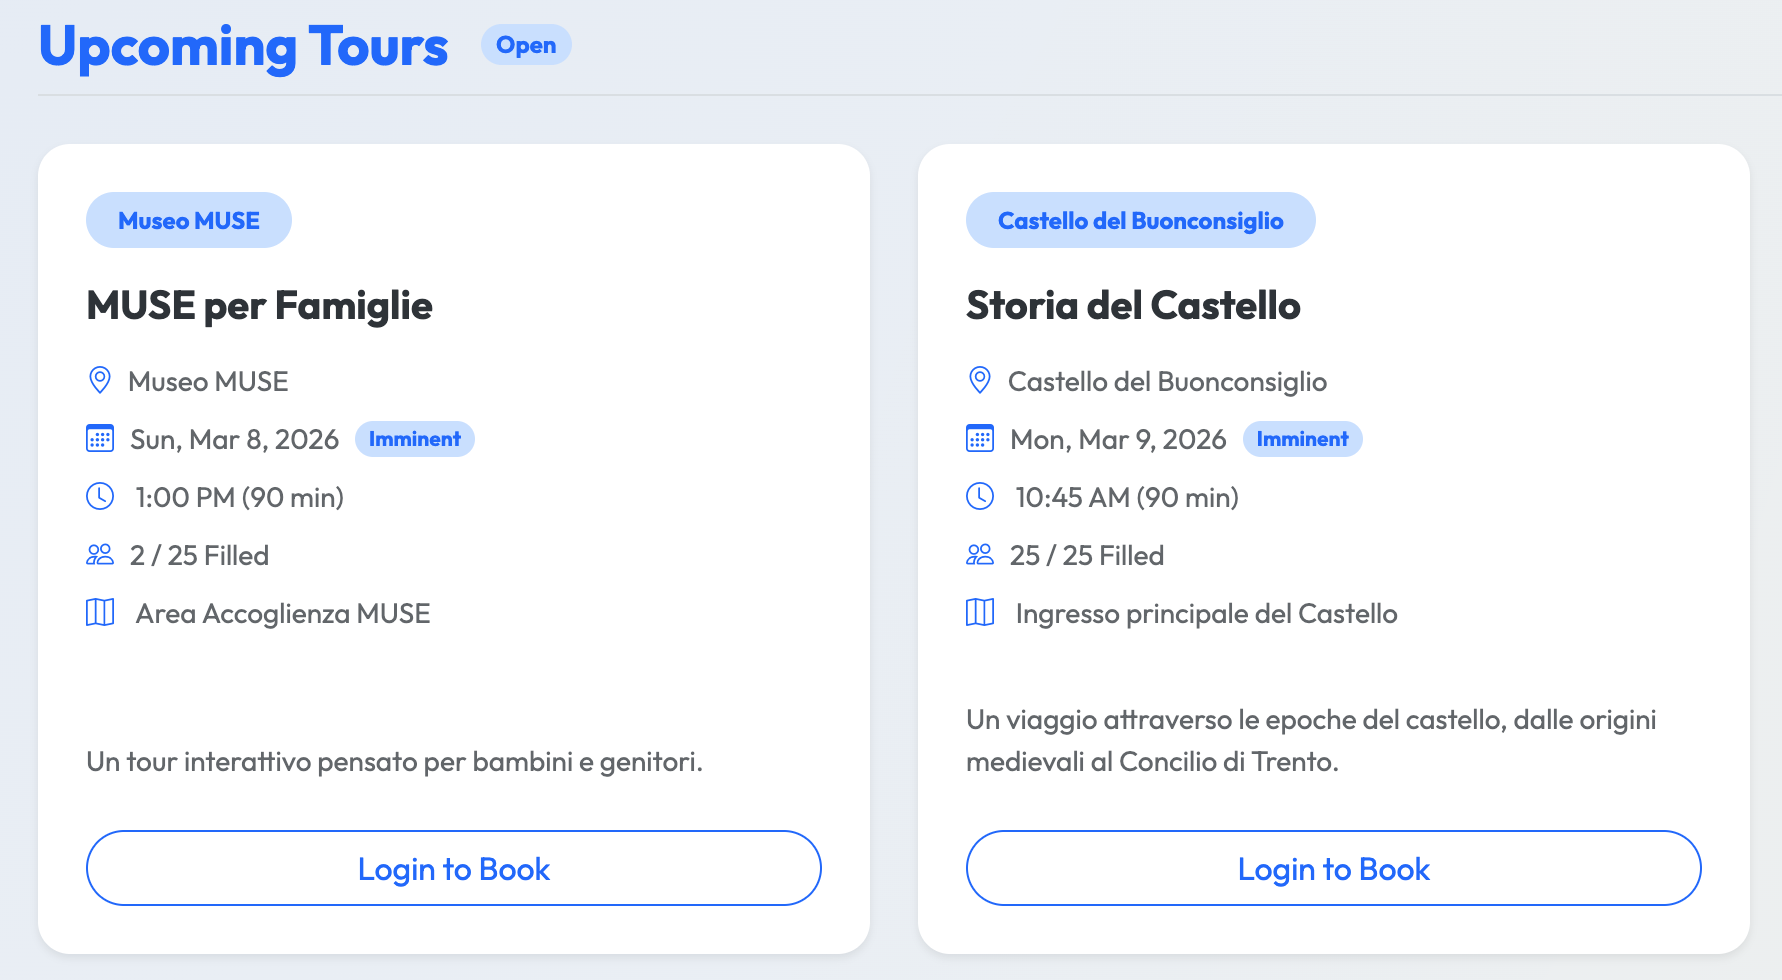
\includegraphics[width=\textwidth, keepaspectratio]{capitoli/immagini/v2/p4_v2.png}
        \caption{V2 (Dopo)}
    \end{subfigure}
    \caption{P.4 -- Inconsistenza cromatica: V1 (stesso stato, colori diversi) vs V2 (badge uniformi).}
    \label{fig:det_p4}
\end{figure}

\noindent\textbf{P.5 \& P.6 -- Chiarezza e stile nota pagamento} \hfill \textit{Severità: 2}

Il messaggio sulle modalità di pagamento era ambiguo e privo di enfasi visiva. In V2 ogni card mostra il prezzo esplicito (\textit{Free} o \textit{€X}) e la nota è presentata come banner \texttt{alert-warning} con icona, ad alto contrasto.

\begin{figure}[H]
    \centering
    \begin{subfigure}[b]{0.47\textwidth}
        \centering
        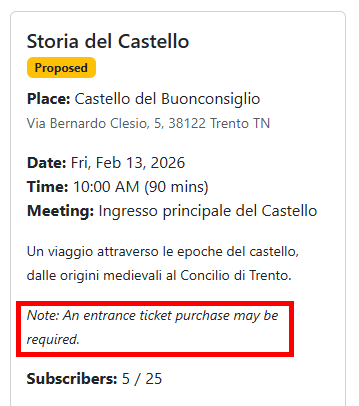
\includegraphics[width=\textwidth, keepaspectratio]{capitoli/immagini/p3.png}
        \caption{V1 (Prima)}
    \end{subfigure}
    \hfill
    \begin{subfigure}[b]{0.47\textwidth}
        \centering
        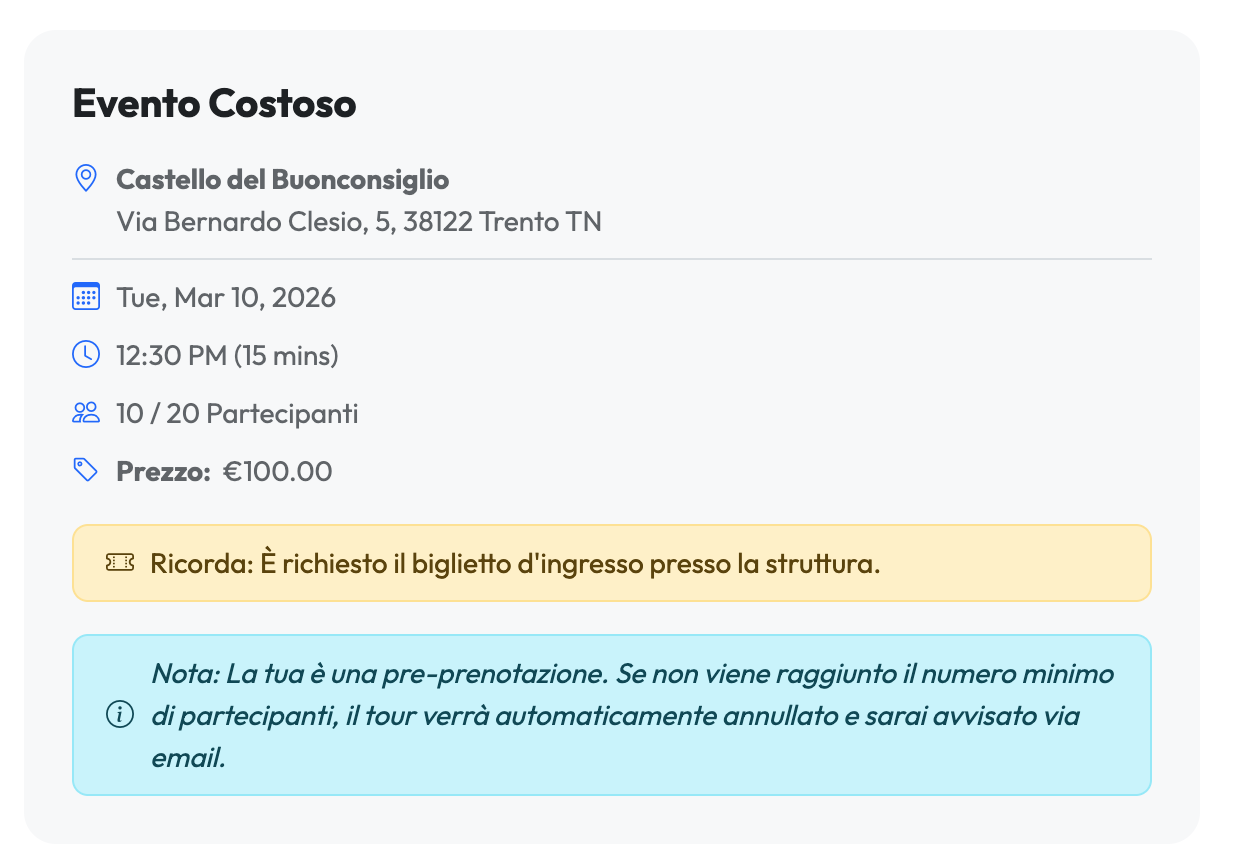
\includegraphics[width=\textwidth, keepaspectratio]{capitoli/immagini/v2/p6_v2.png}
        \caption{V2 (Dopo)}
    \end{subfigure}
    \caption{P.5/P.6 -- Nota pagamento: V1 (testo generico) vs V2 (prezzo esplicito e banner warning).}
    \label{fig:det_p5}
\end{figure}

\noindent\textbf{P.7 -- Ambiguità cromatica stati visita} \hfill \textit{Severità: 1}

"Confirmed" e "Complete" condividevano la stessa tinta verde. In V2 "Confirmed" mantiene \texttt{bg-success} (verde), "Complete" usa \texttt{bg-secondary} (grigio): la distinzione cromatica è immediata.

\begin{figure}[H]
    \centering
    \begin{subfigure}[b]{0.47\textwidth}
        \centering
        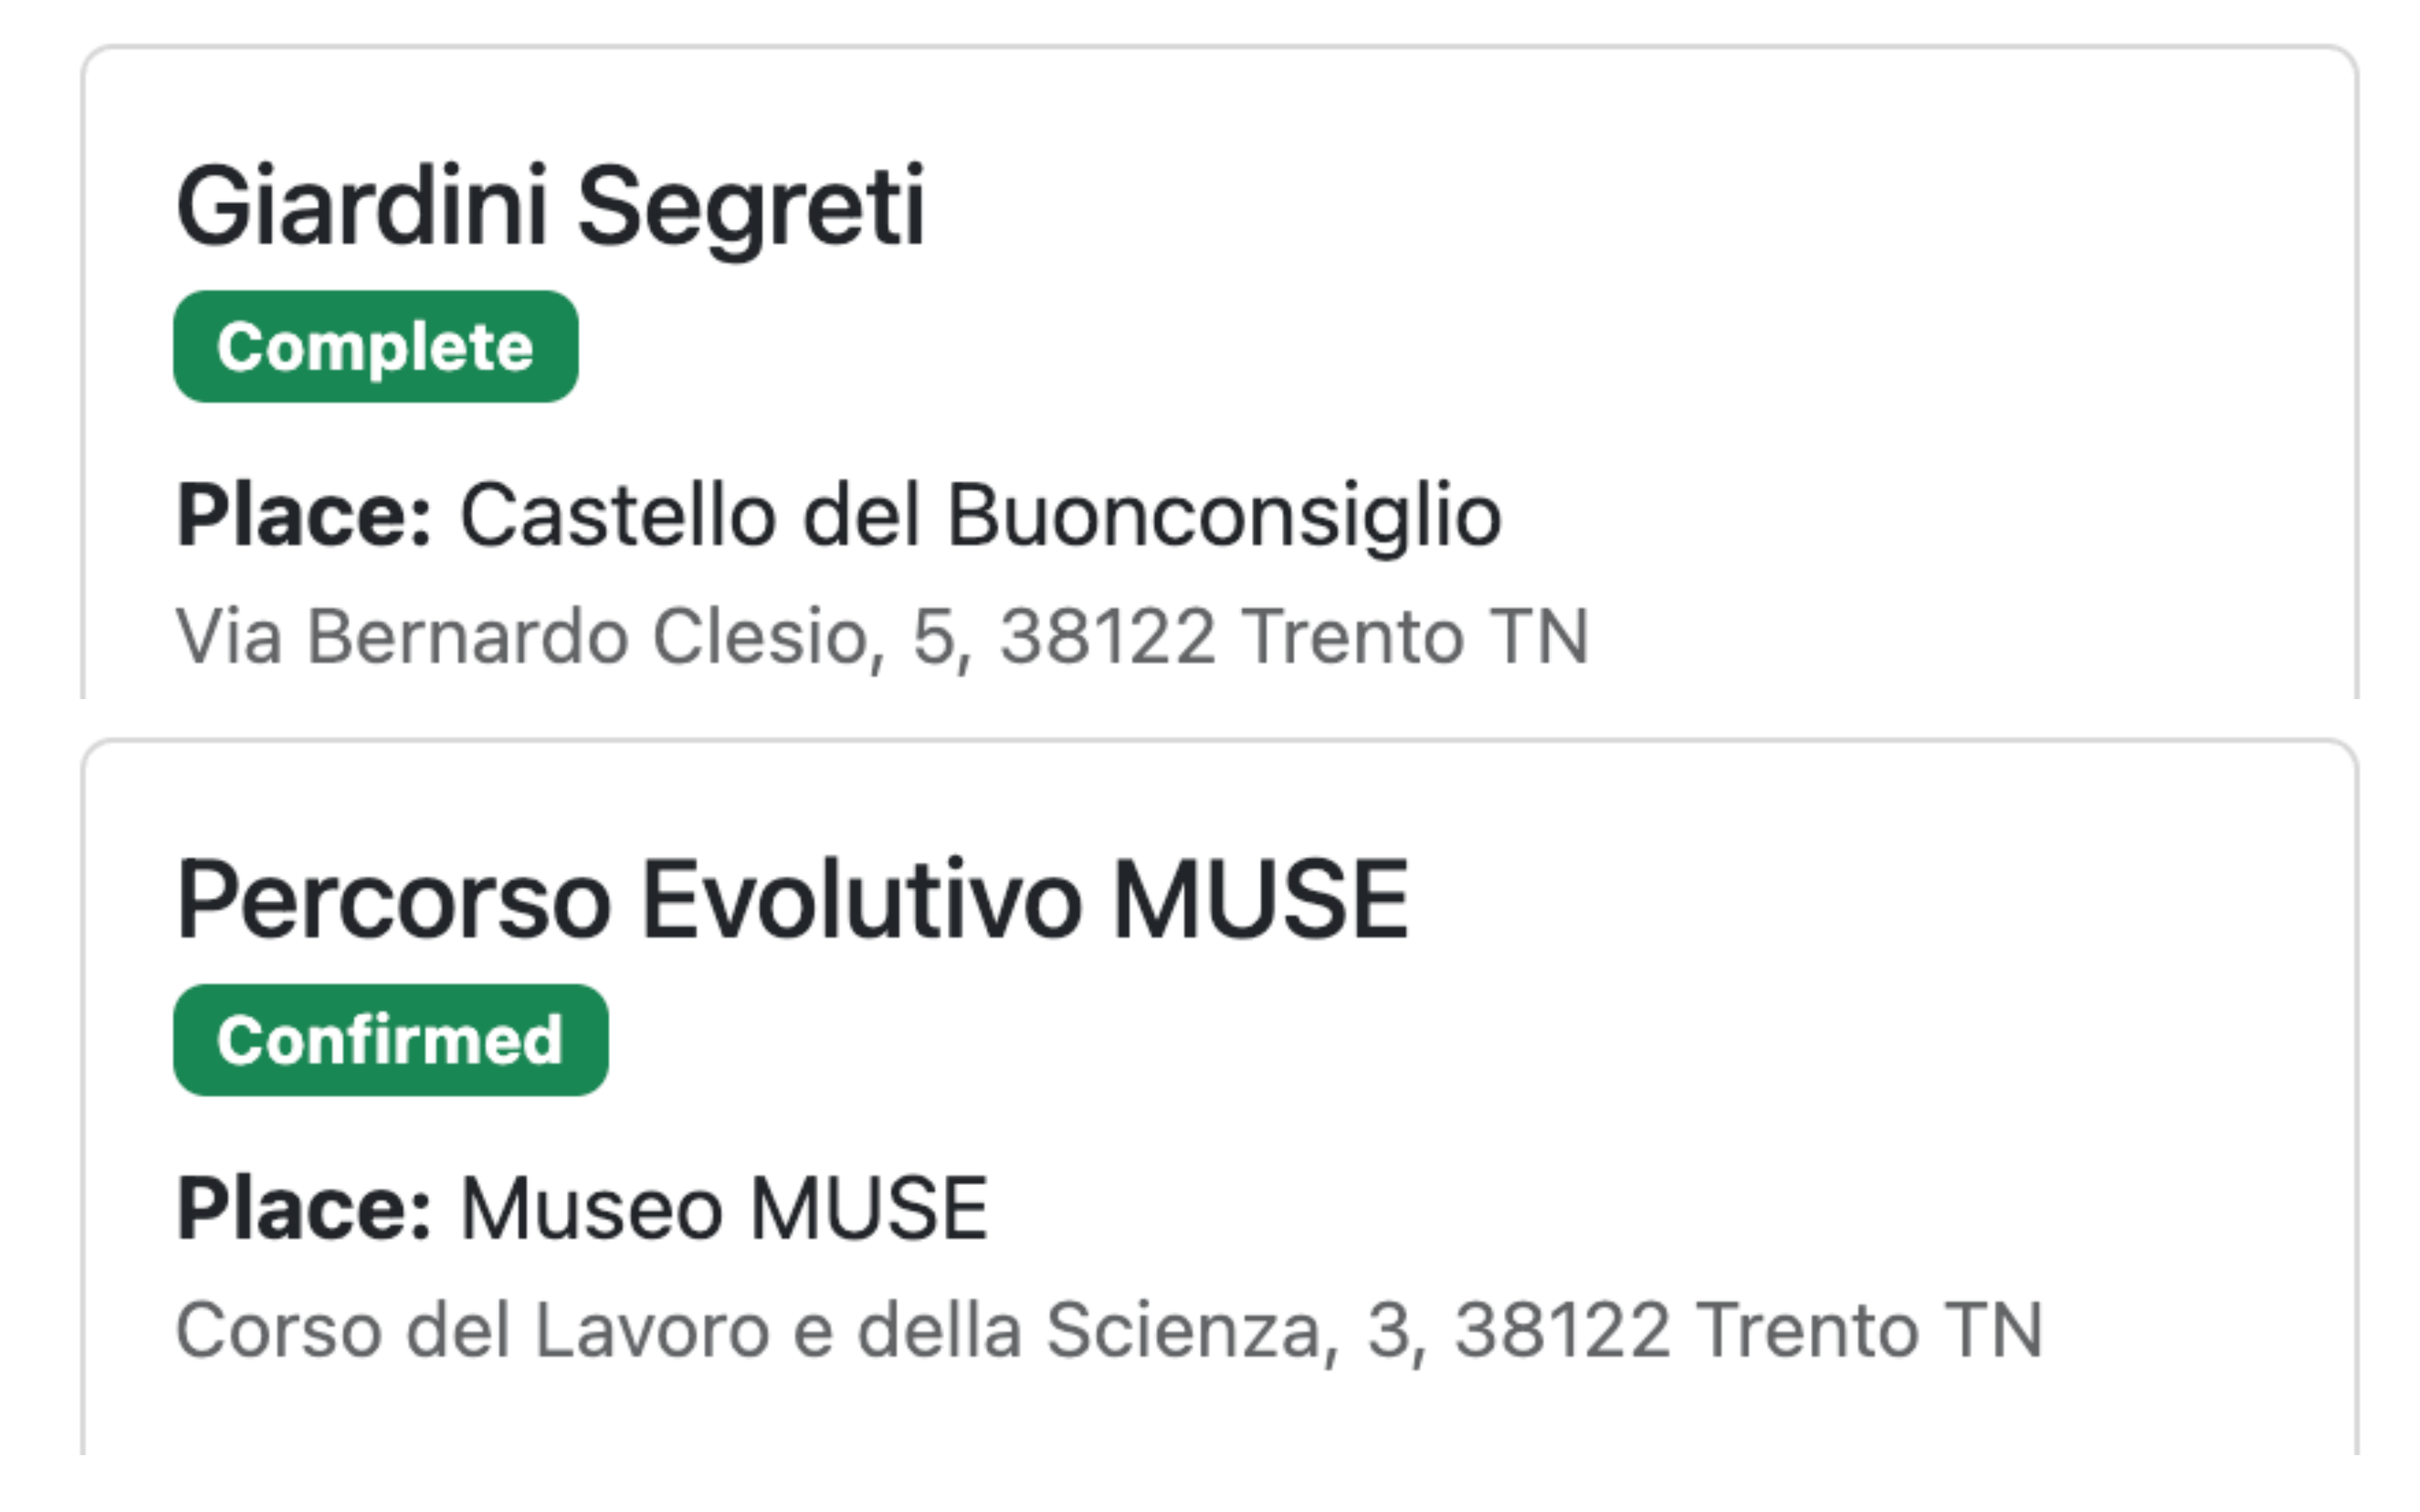
\includegraphics[width=\textwidth, keepaspectratio]{capitoli/immagini/p4.png}
        \caption{V1 (Prima)}
    \end{subfigure}
    \hfill
    \begin{subfigure}[b]{0.47\textwidth}
        \centering
        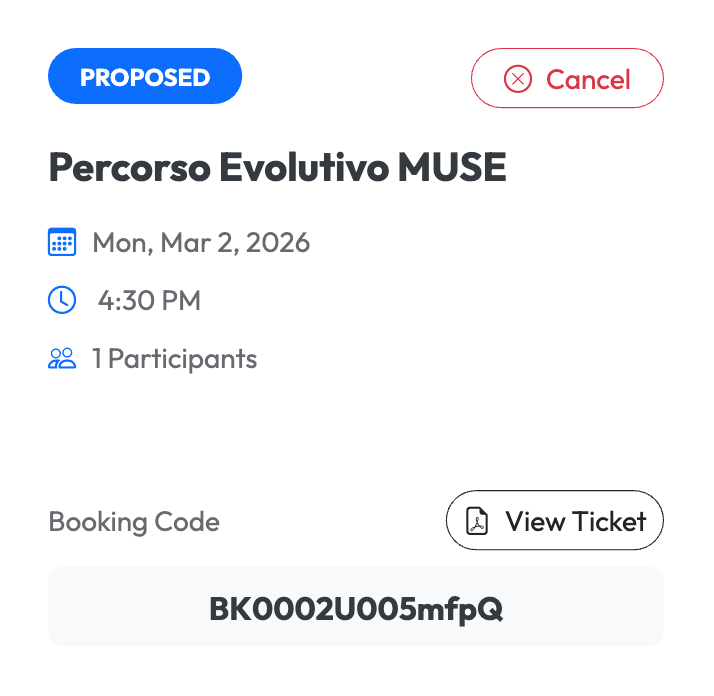
\includegraphics[width=\textwidth, keepaspectratio]{capitoli/immagini/v2/p7_v2.png}
        \caption{V2 (Dopo)}
    \end{subfigure}
    \caption{P.7 -- Ambiguità cromatica: V1 (badge identici) vs V2 (verde futuro, grigio passato).}
    \label{fig:det_p7}
\end{figure}

\noindent\textbf{P.8 -- Mancanza feedback disponibilità} \hfill \textit{Severità: 1}

Nessun indicatore visivo segnalava la saturazione delle visite. In V2 ogni card mostra il contatore "X/Y Filled" e il badge "Filling Fast" quando i posti scendono sotto soglia critica.

\begin{figure}[H]
    \centering
    \begin{subfigure}[b]{0.47\textwidth}
        \centering
        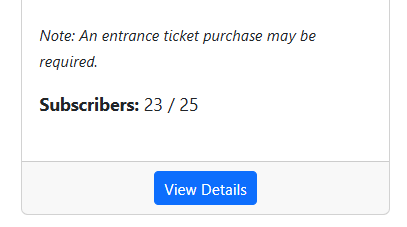
\includegraphics[width=\textwidth, keepaspectratio]{capitoli/immagini/p6.png}
        \caption{V1 (Prima)}
    \end{subfigure}
    \hfill
    \begin{subfigure}[b]{0.47\textwidth}
        \centering
        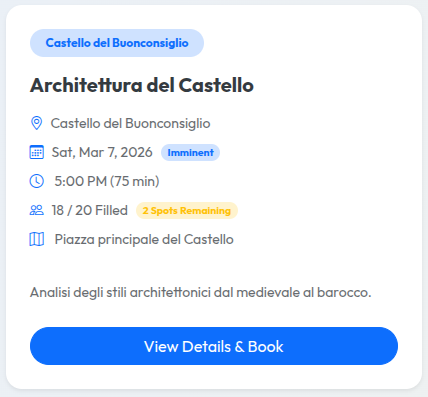
\includegraphics[width=\textwidth, keepaspectratio]{capitoli/immagini/v2/p3_v2.png}
        \caption{V2 (Dopo)}
    \end{subfigure}
    \caption{P.8 -- Feedback disponibilità: V1 (nessun indicatore) vs V2 (contatore posti e badge "Filling Fast").}
    \label{fig:det_p8}
\end{figure}

\noindent\textbf{P.9 -- Ridondanza "Visite confermate"} \hfill \textit{Severità: 1}

La sezione delle visite confermate risultava confusa. In V2 le sezioni "Upcoming" e "Your Confirmed" sono distinte con intestazioni esplicite che ne chiariscono il contenuto.

\begin{figure}[H]
    \centering
    \begin{subfigure}[b]{0.47\textwidth}
        \centering
        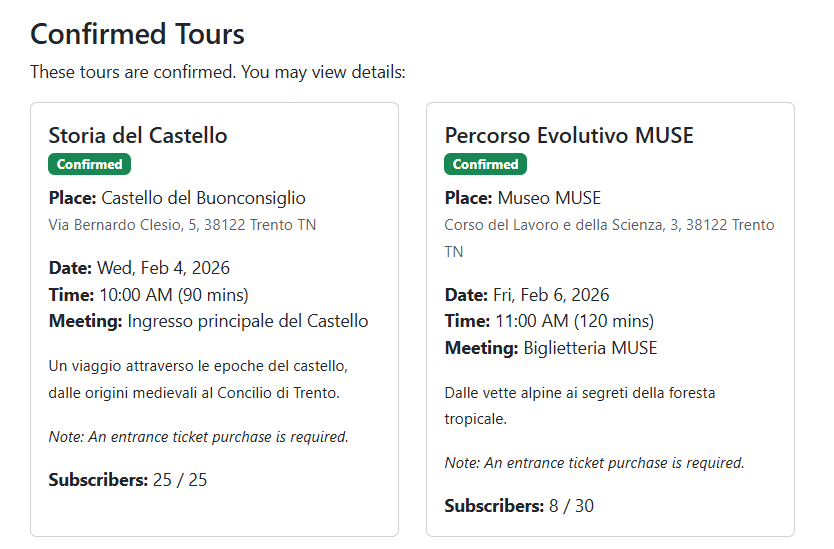
\includegraphics[width=\textwidth, keepaspectratio]{capitoli/immagini/p7.png}
        \caption{V1 (Prima)}
    \end{subfigure}
    \hfill
    \begin{subfigure}[b]{0.47\textwidth}
        \centering
        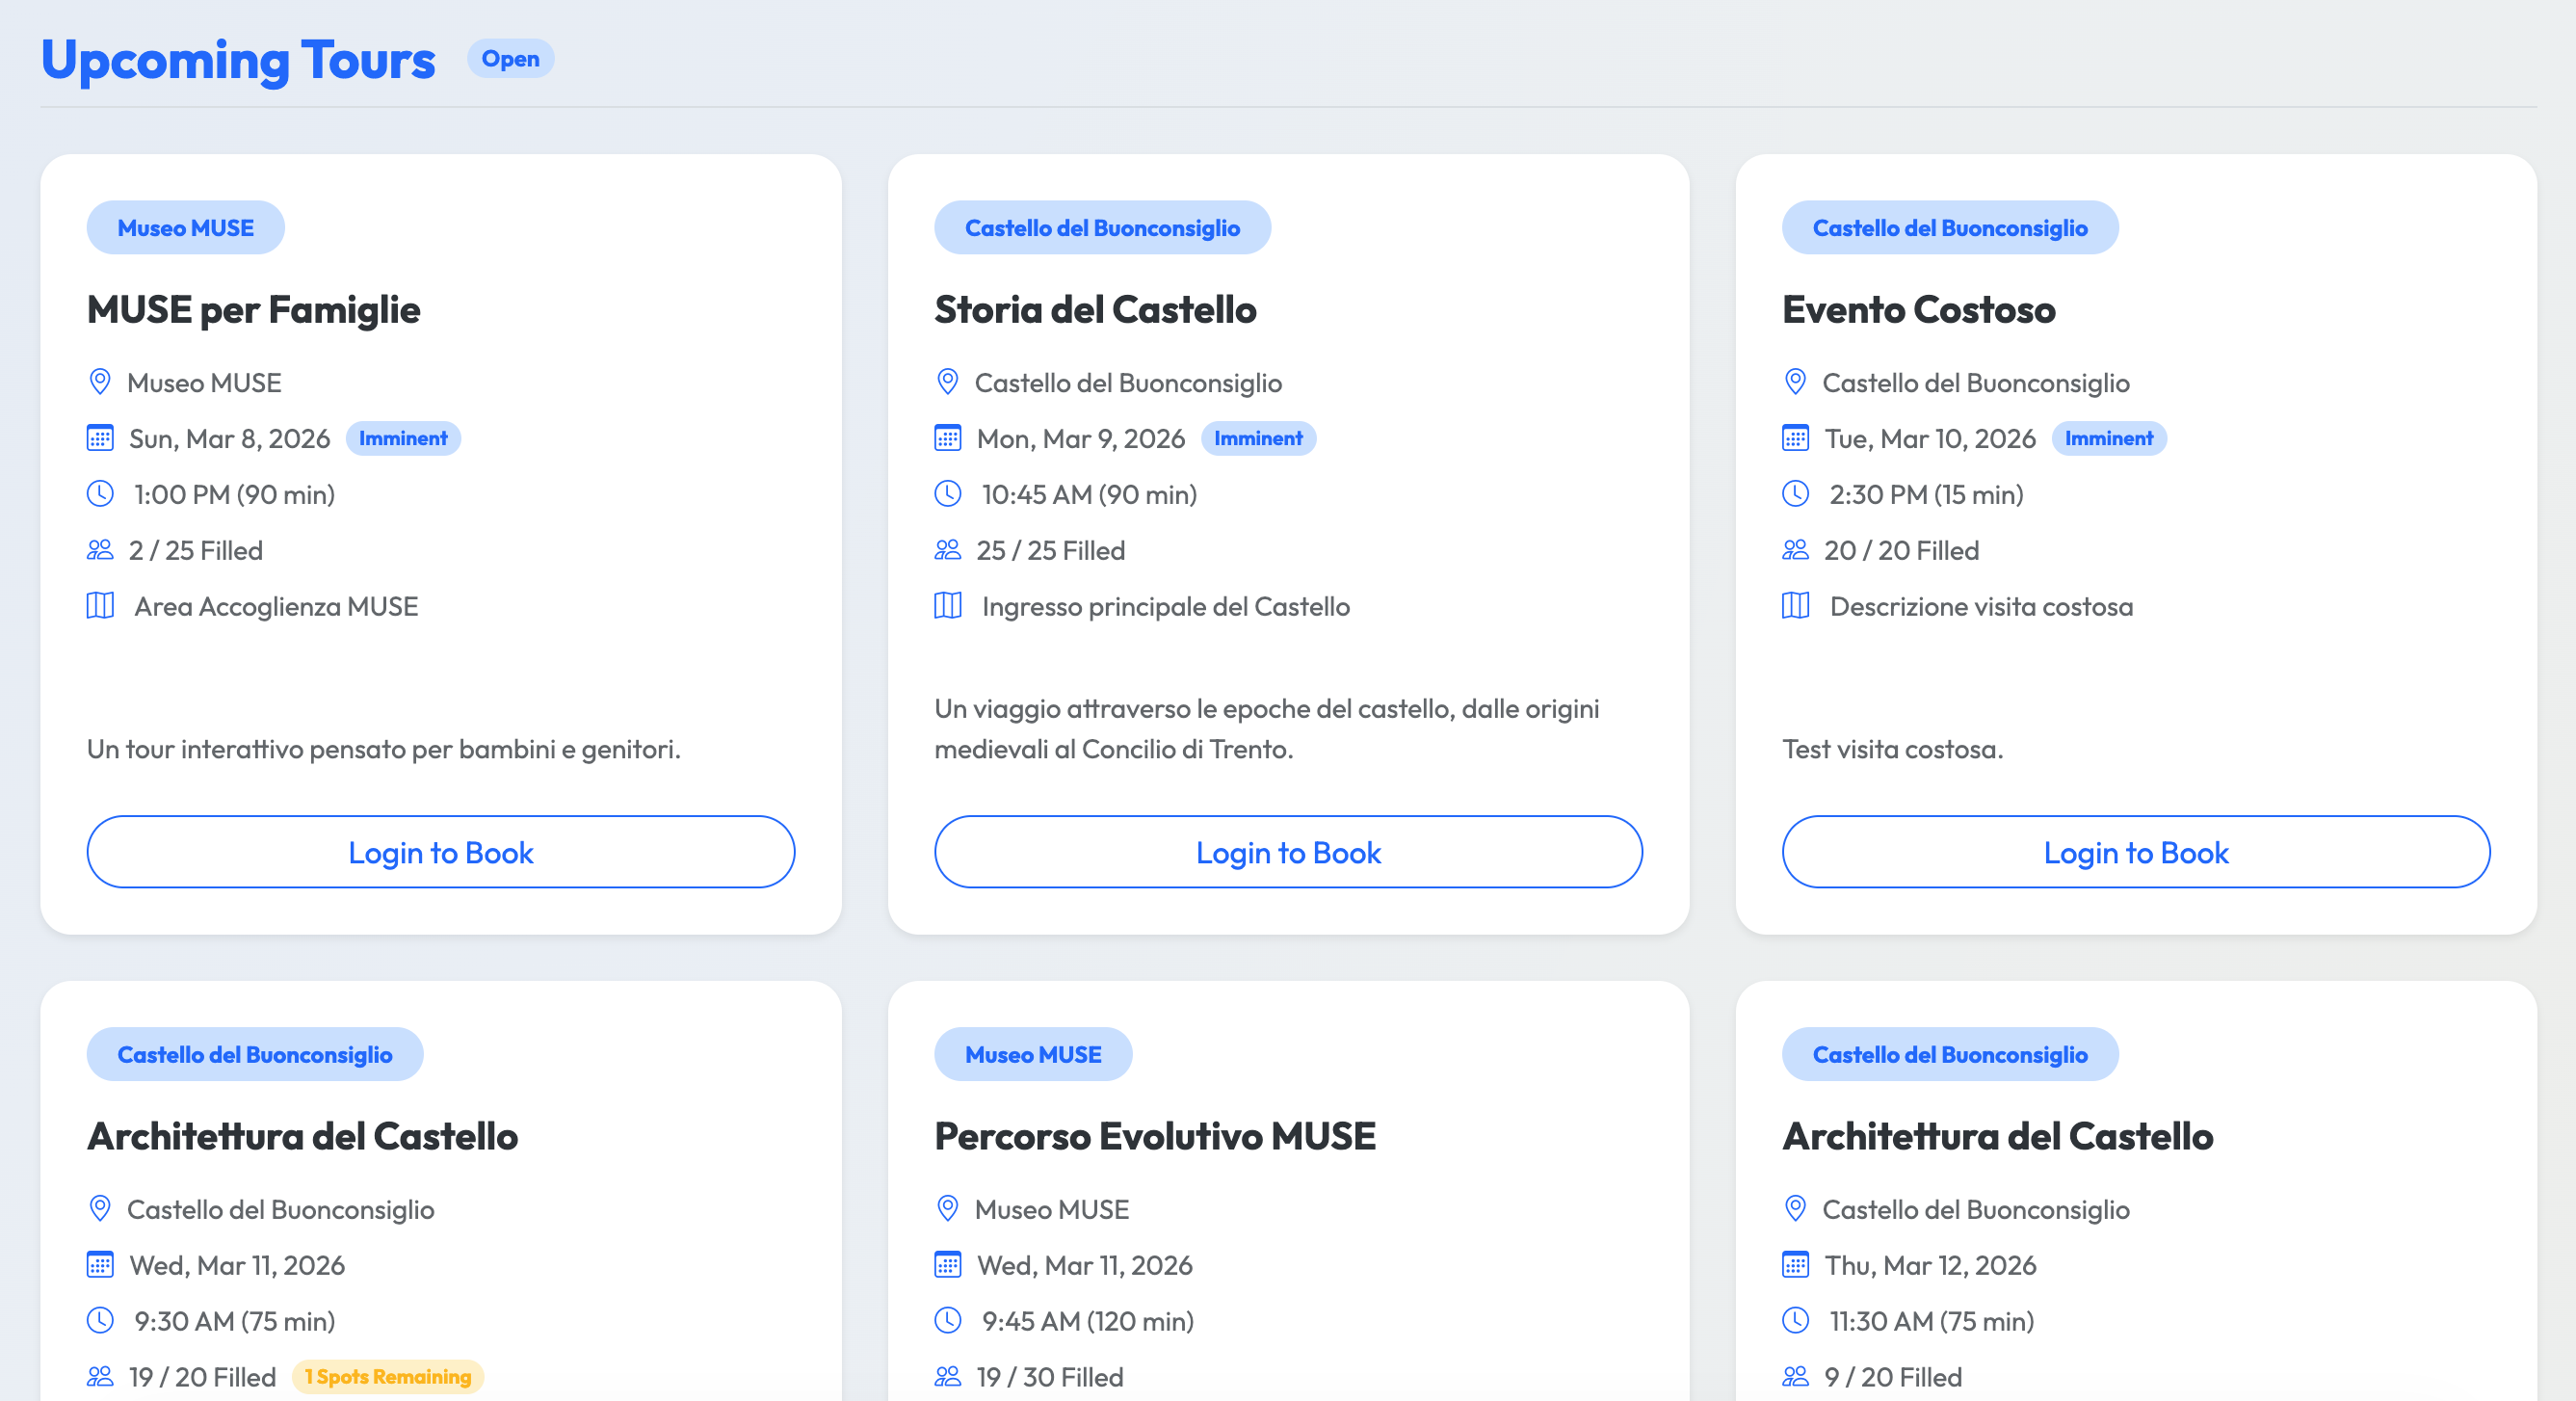
\includegraphics[width=\textwidth, keepaspectratio]{capitoli/immagini/v2/p9_v2.png}
        \caption{V2 (Dopo)}
    \end{subfigure}
    \caption{P.9 -- Sezioni homepage: V1 (struttura confusa) vs V2 (sezioni distinte con titoli chiari).}
    \label{fig:det_p9}
\end{figure}

\noindent\textbf{P.10 -- Area cliccabile limitata} \hfill \textit{Severità: 2}

L'accesso ai dettagli era vincolato al solo pulsante della card. In V2 l'intera card è cliccabile tramite \texttt{stretched-link} Bootstrap, con effetto hover visivo tramite classe \texttt{card-hover}.

\begin{figure}[H]
    \centering
    \begin{subfigure}[b]{0.47\textwidth}
        \centering
        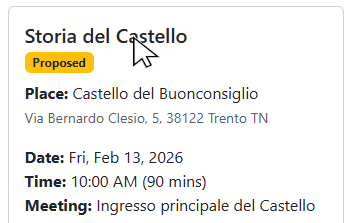
\includegraphics[width=\textwidth, keepaspectratio]{capitoli/immagini/p8.png}
        \caption{V1 (Prima)}
    \end{subfigure}
    \hfill
    \begin{subfigure}[b]{0.47\textwidth}
        \centering
        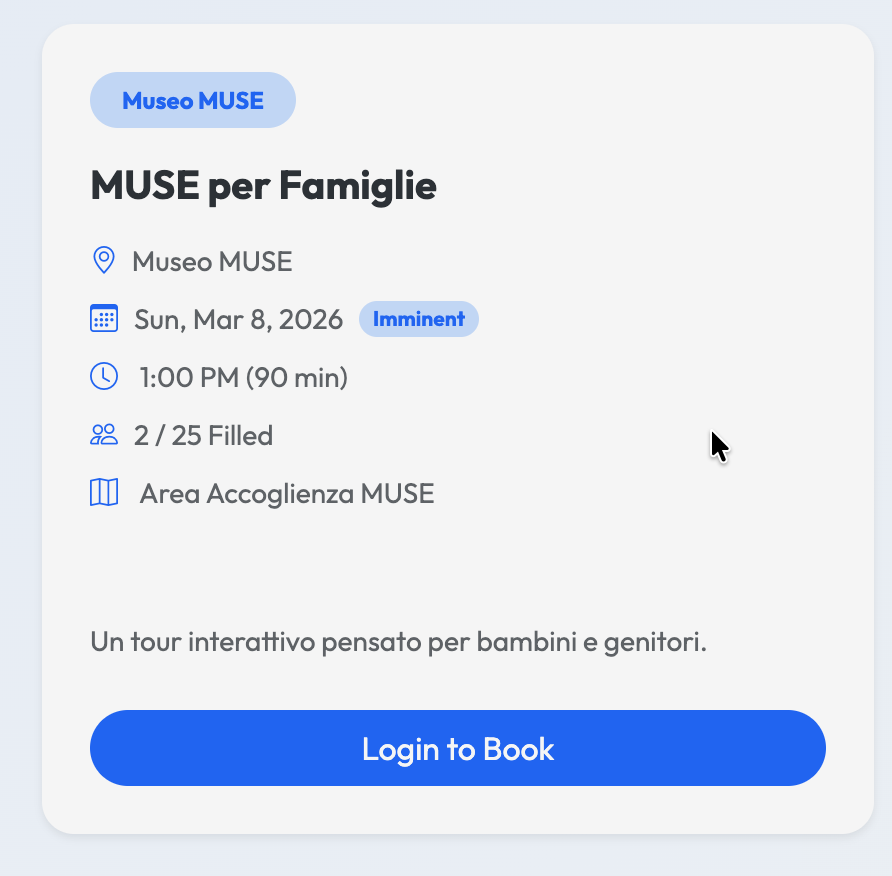
\includegraphics[width=\textwidth, keepaspectratio]{capitoli/immagini/v2/p10_v2.png}
        \caption{V2 (Dopo)}
    \end{subfigure}
    \caption{P.10 -- Area cliccabile: V1 (solo bottone) vs V2 (intera card interattiva con hover).}
    \label{fig:det_p10}
\end{figure}

\noindent\textbf{P.11 -- Gerarchia visiva debole} \hfill \textit{Severità: 1}

La gerarchia tipografica era appiattita. In V2 è implementata una scala chiara: \texttt{display-4} per il titolo hero, \texttt{h3} per le sezioni, \texttt{h5} per i sottotitoli delle card.

\begin{figure}[H]
    \centering
    \begin{subfigure}[b]{0.47\textwidth}
        \centering
        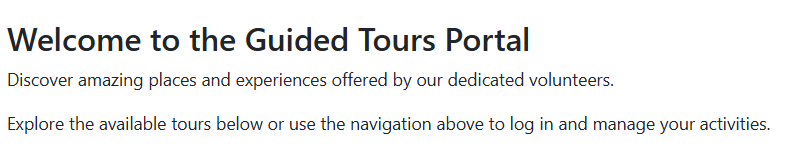
\includegraphics[width=\textwidth, keepaspectratio]{capitoli/immagini/p9.png}
        \caption{V1 (Prima)}
    \end{subfigure}
    \hfill
    \begin{subfigure}[b]{0.47\textwidth}
        \centering
        
\includegraphics[width=\textwidth, keepaspectratio]{capitoli/immagini/v2/p11_v2.png}
        \caption{V2 (Dopo)}
    \end{subfigure}
    \caption{P.11 -- Gerarchia visiva: V1 (gerarchia debole) vs V2 (tipografia \texttt{display-4} con forte contrasto).}
    \label{fig:det_p11}
\end{figure}

\noindent\textbf{P.12 -- Assenza shortcut area personale} \hfill \textit{Severità: 1}

Dalla homepage mancava un accesso diretto alla propria area personale. In V2 l'hero section include, per gli utenti autenticati come Customer, un bottone "My Dashboard" per raggiungerla in un click.

\begin{figure}[H]
    \centering
    \begin{subfigure}[b]{0.47\textwidth}
        \centering
        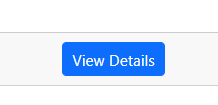
\includegraphics[width=\textwidth, keepaspectratio]{capitoli/immagini/p10.png}
        \caption{V1 (Prima)}
    \end{subfigure}
    \hfill
    \begin{subfigure}[b]{0.47\textwidth}
        \centering
        
\includegraphics[width=\textwidth, keepaspectratio]{capitoli/immagini/v2/p12_v2.png}
        \caption{V2 (Dopo)}
    \end{subfigure}
    \caption{P.12 -- Shortcut area personale: V1 (nessun accesso rapido) vs V2 (bottone "My Dashboard" nell'hero).}
    \label{fig:det_p12}
\end{figure}

\subsection{Footer e Navbar}

\noindent\textbf{P.13 -- Incoerenza linguistica} \hfill \textit{Severità: 1}

Il footer conteneva la dicitura italiana "Sito di visite guidate" in un'interfaccia altrimenti in inglese. In V2 l'intero footer è riscritto in inglese.

\begin{figure}[H]
    \centering
    \begin{subfigure}[b]{0.47\textwidth}
        \centering
        
\includegraphics[width=\textwidth, keepaspectratio]{capitoli/immagini/p12.png}
        \caption{V1 (Prima)}
    \end{subfigure}
    \hfill
    \begin{subfigure}[b]{0.47\textwidth}
        \centering
        
\includegraphics[width=\textwidth, keepaspectratio]{capitoli/immagini/v2/p13_v2.png}
        \caption{V2 (Dopo)}
    \end{subfigure}
    \caption{P.13 -- Incoerenza linguistica: V1 (testo italiano nel footer) vs V2 (footer interamente in inglese).}
    \label{fig:det_p13}
\end{figure}

\noindent\textbf{P.35 -- Email non cliccabili} \hfill \textit{Severità: 2}

Gli indirizzi email nel footer non erano cliccabili nonostante l'aspetto da link. In V2 sono avvolti da tag \texttt{<a href="mailto:...">} e stilizzati coerentemente.

\begin{figure}[H]
    \centering
    \begin{subfigure}[b]{0.47\textwidth}
        \centering
        
\includegraphics[width=\textwidth, keepaspectratio]{capitoli/immagini/p33.png}
        \caption{V1 (Prima)}
    \end{subfigure}
    \hfill
    \begin{subfigure}[b]{0.47\textwidth}
        \centering
        
\includegraphics[width=\textwidth, keepaspectratio]{capitoli/immagini/v2/p35_v2.png}
        \caption{V2 (Dopo)}
    \end{subfigure}
    \caption{P.35 -- Email cliccabili: V1 (testo statico) vs V2 (link \texttt{mailto} attivi).}
    \label{fig:det_p35}
\end{figure}

\subsection{Autenticazione (Login e Register)}

\noindent\textbf{P.15 -- Mancanza toggle visibilità password} \hfill \textit{Severità: 1}

L'assenza di un toggle per visualizzare la password aumentava la probabilità di errori di digitazione. In V2 è presente un'icona occhio con script \texttt{showPassword()} nelle pagine Login e Register.

\begin{figure}[H]
    \centering
    \begin{subfigure}[b]{0.47\textwidth}
        \centering
        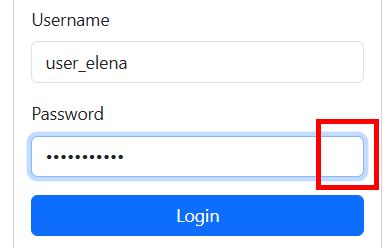
\includegraphics[width=\textwidth, keepaspectratio]{capitoli/immagini/p11.png}
        \caption{V1 (Prima)}
    \end{subfigure}
    \hfill
    \begin{subfigure}[b]{0.47\textwidth}
        \centering
        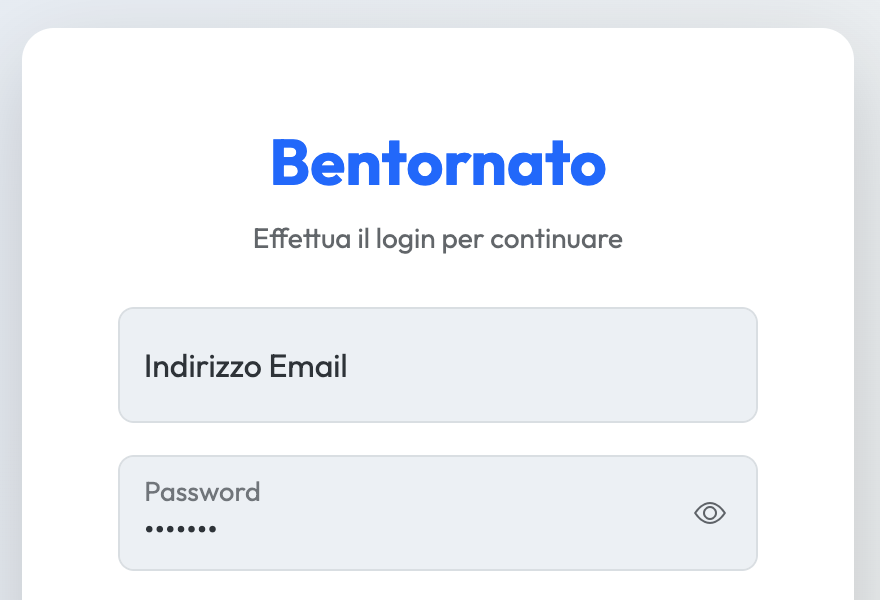
\includegraphics[width=\textwidth, keepaspectratio]{capitoli/immagini/v2/p15_v2.png}
        \caption{V2 (Dopo)}
    \end{subfigure}
    \caption{P.15 -- Toggle password: V1 (campo senza icona) vs V2 (icona occhio attiva).}
    \label{fig:det_p15}
\end{figure}

\noindent\textbf{P.16 \& P.17 -- Navigazione ambigua e ridondanza ruoli (Login)} \hfill \textit{Severità: 1}

La pagina di login presentava link multipli e testo ridondante sui ruoli. In V2 rimane un solo link "Create an Account" e il testo è ridotto all'essenziale.

\begin{figure}[H]
    \centering
    \begin{subfigure}[b]{0.47\textwidth}
        \centering
        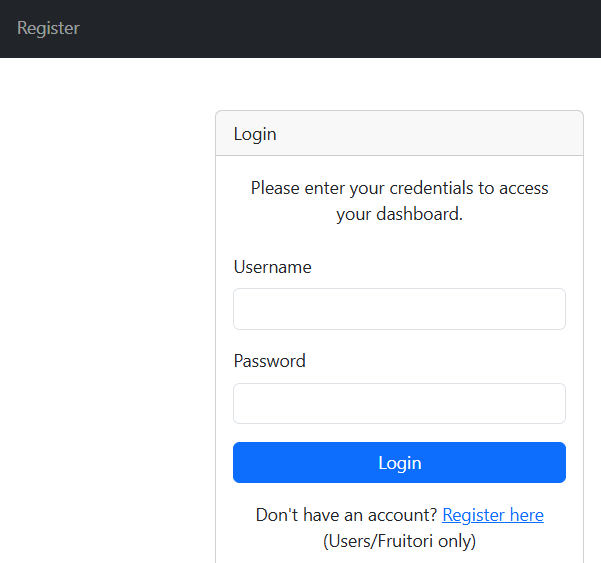
\includegraphics[width=\textwidth, keepaspectratio]{capitoli/immagini/p14.png}
        \caption{V1 (Prima)}
    \end{subfigure}
    \hfill
    \begin{subfigure}[b]{0.47\textwidth}
        \centering
        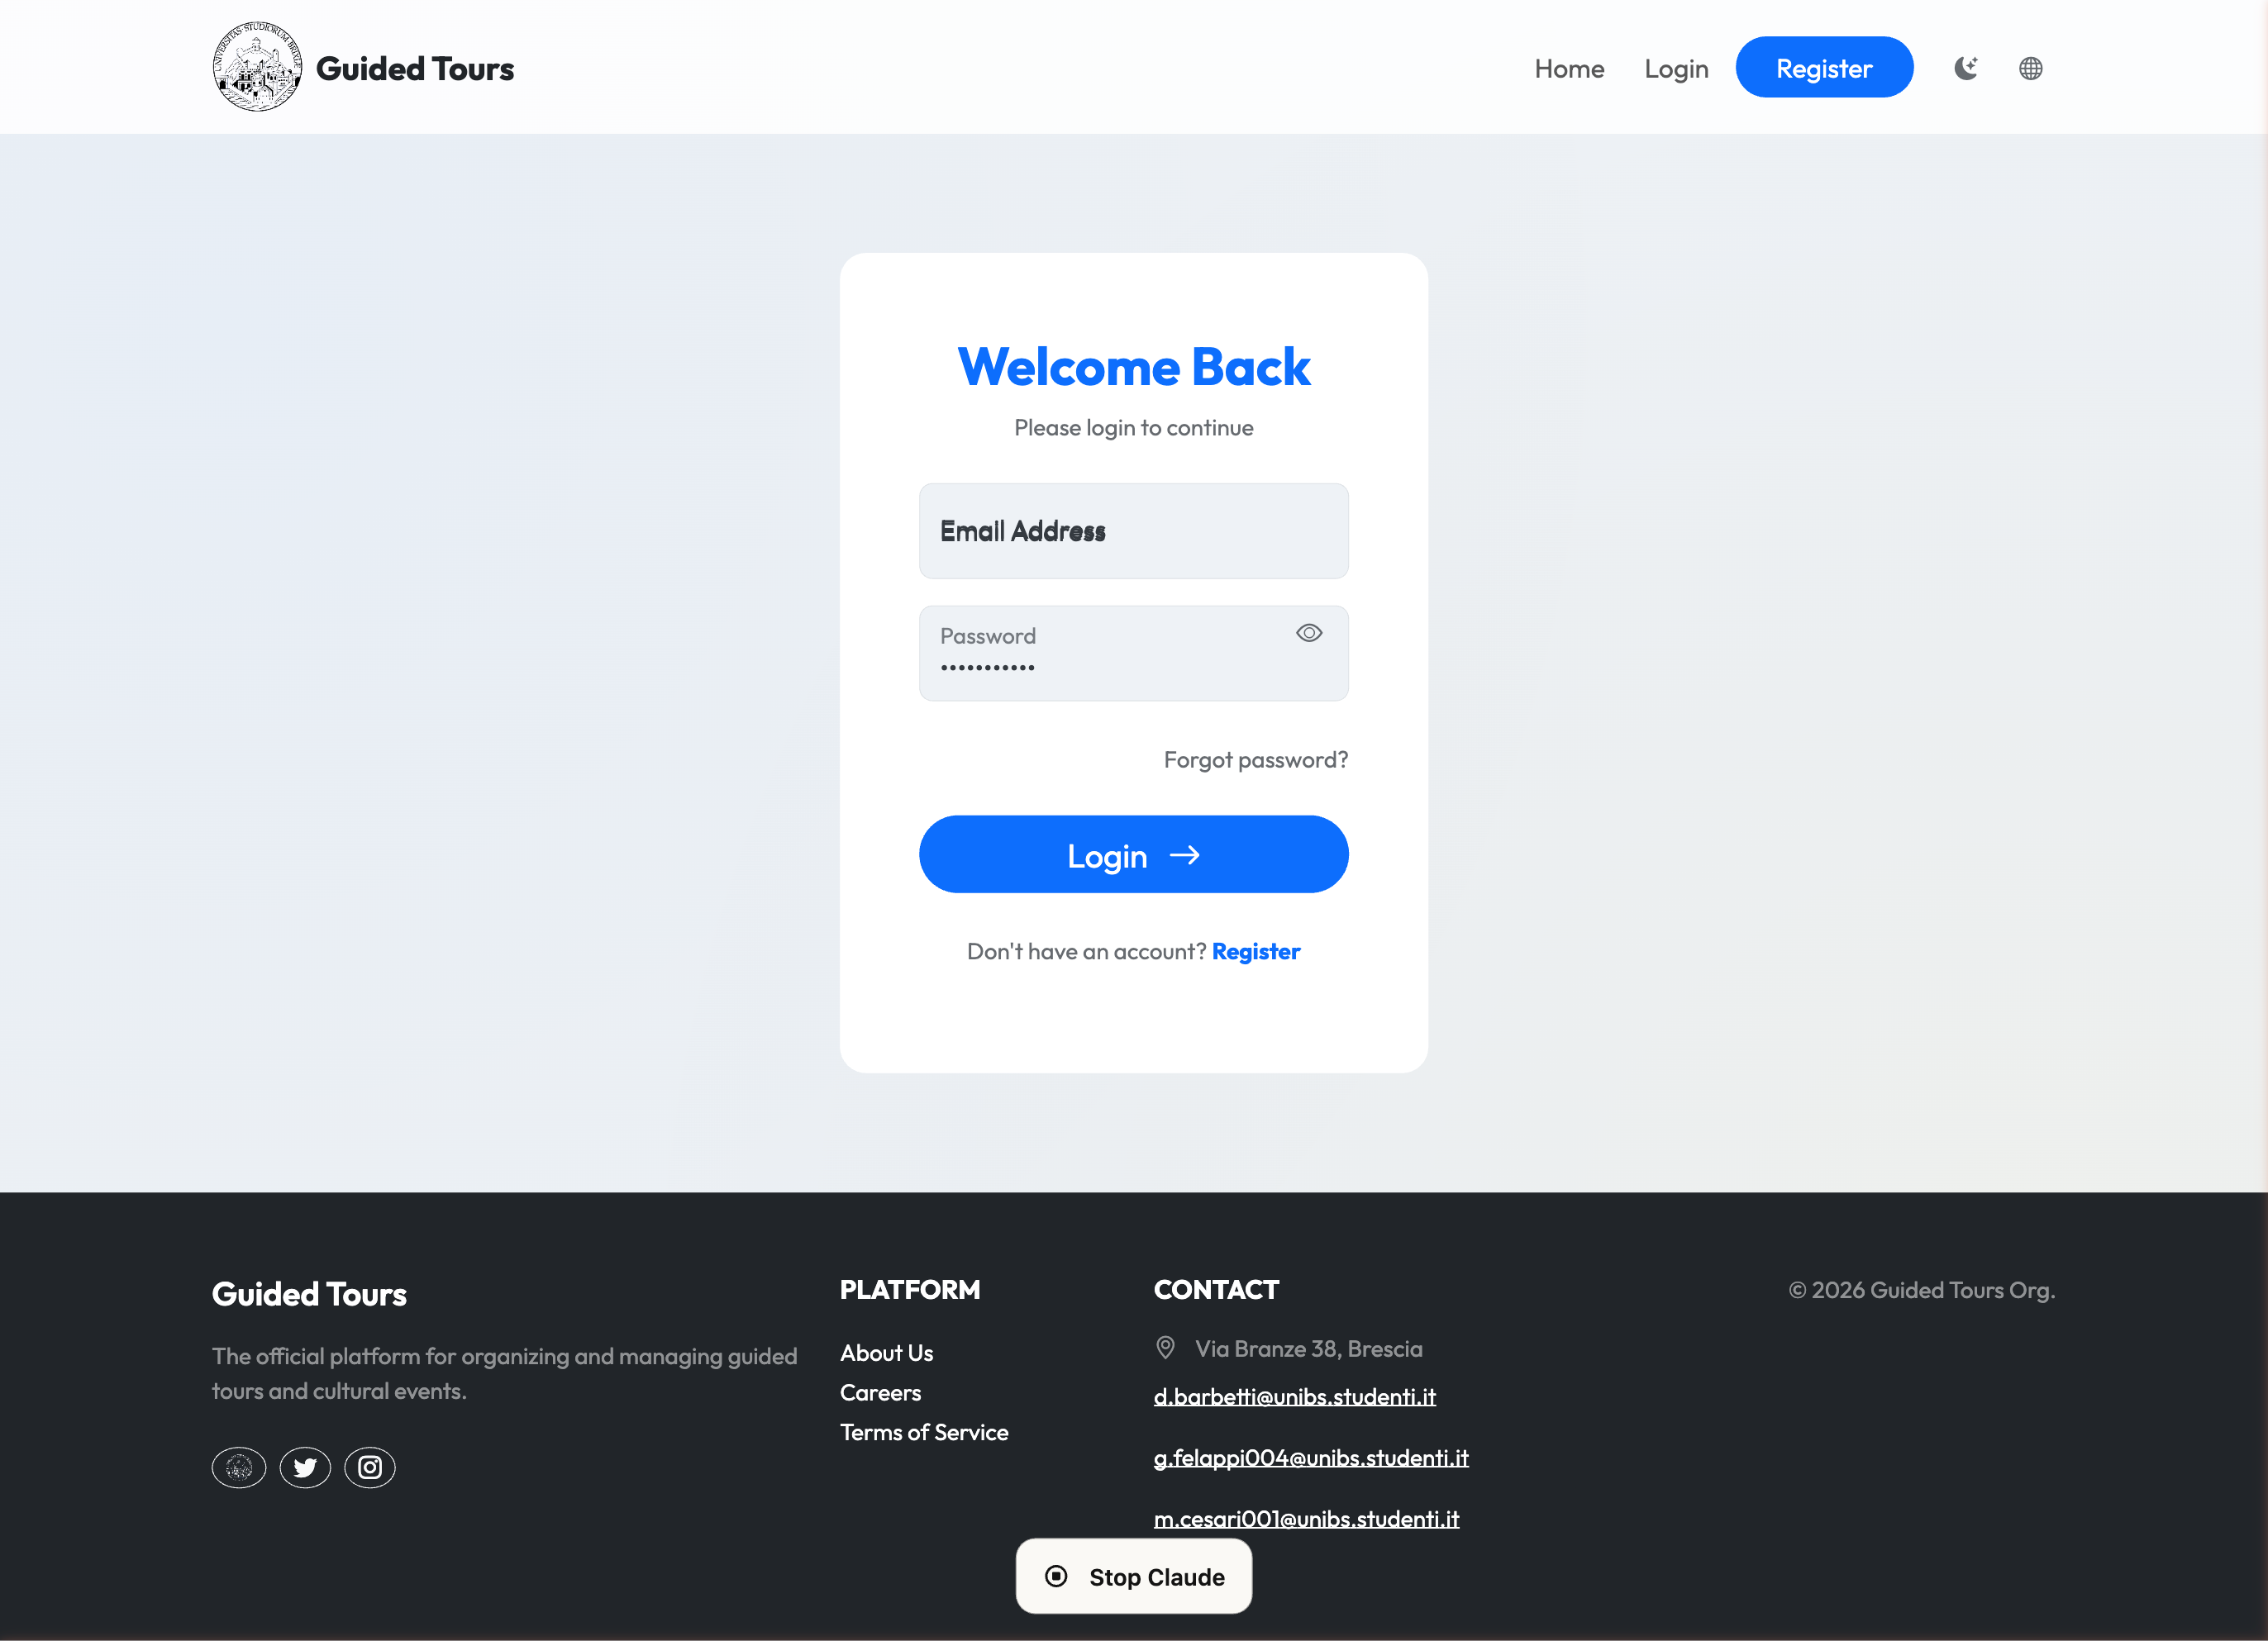
\includegraphics[width=\textwidth, keepaspectratio]{capitoli/immagini/v2/p16_v2.png}
        \caption{V2 (Dopo)}
    \end{subfigure}
    \caption{P.16/P.17 -- Login: V1 (link multipli e testo ridondante) vs V2 (form pulito con link unico).}
    \label{fig:det_p16}
\end{figure}

\noindent\textbf{P.18 -- Feedback errore non user-friendly} \hfill \textit{Severità: 1}

I messaggi di errore in caso di credenziali errate erano tecnici e poco comprensibili. In V2 sono presentati tramite Toast Notifications con testo chiaro e contestuale.

\begin{figure}[H]
    \centering
    \begin{subfigure}[b]{0.47\textwidth}
        \centering
        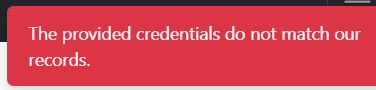
\includegraphics[width=\textwidth, keepaspectratio]{capitoli/immagini/p16.png}
        \caption{V1 (Prima)}
    \end{subfigure}
    \hfill
    \begin{subfigure}[b]{0.47\textwidth}
        \centering
        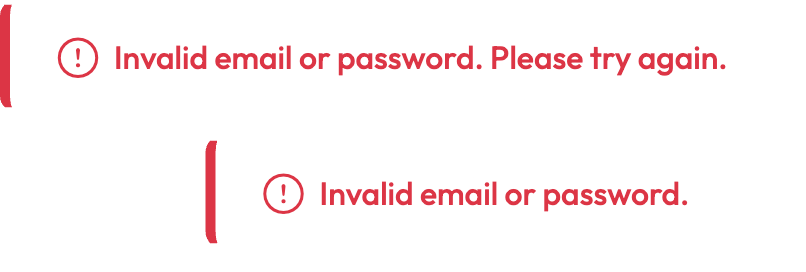
\includegraphics[width=\textwidth, keepaspectratio]{capitoli/immagini/v2/p18_v2.png}
        \caption{V2 (Dopo)}
    \end{subfigure}
    \caption{P.18 -- Feedback errore: V1 (messaggio tecnico) vs V2 (Toast Notification chiara).}
    \label{fig:det_p18}
\end{figure}

\noindent\textbf{P.19 -- Assenza recupero password} \hfill \textit{Severità: 3}

La mancanza di un meccanismo di recupero delle credenziali bloccava l'utente in caso di smarrimento. In V2 è implementata una pagina "Forgot Password" con reset tramite link inviato via email.

\begin{figure}[H]
    \centering
    \begin{subfigure}[b]{0.47\textwidth}
        \centering
        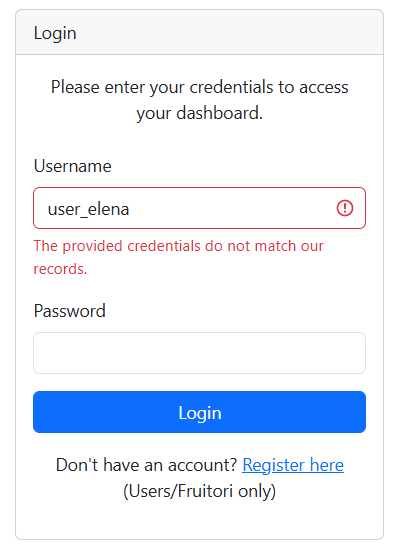
\includegraphics[width=\textwidth, keepaspectratio]{capitoli/immagini/p17.png}
        \caption{V1 (Prima)}
    \end{subfigure}
    \hfill
    \begin{subfigure}[b]{0.47\textwidth}
        \centering
        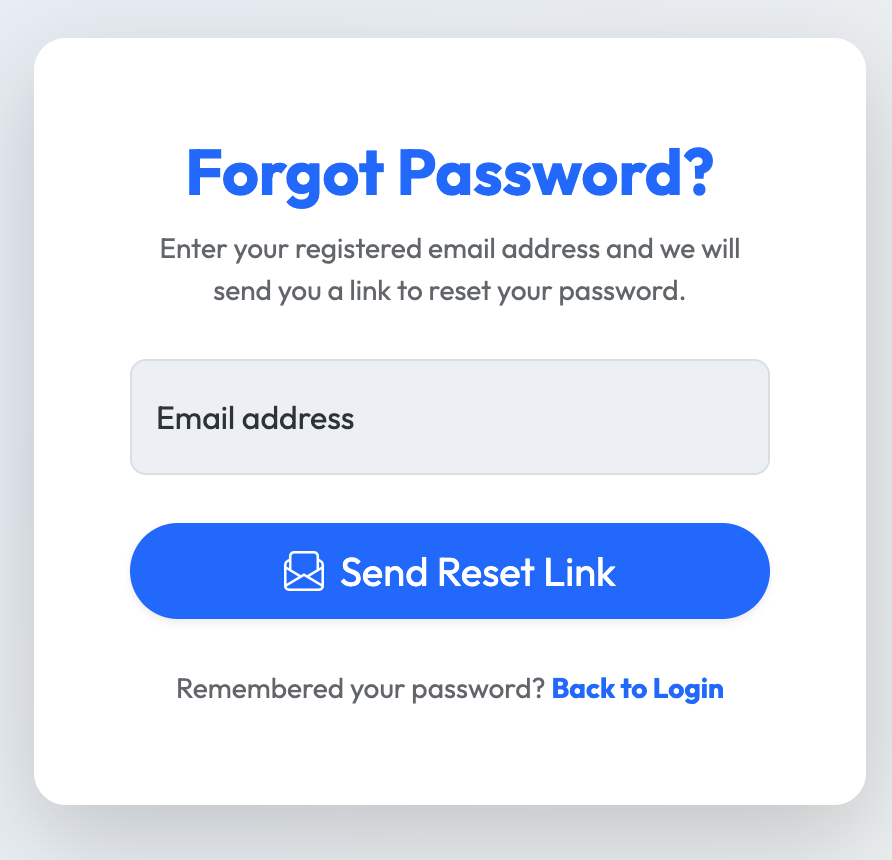
\includegraphics[width=\textwidth, keepaspectratio]{capitoli/immagini/v2/p19_v2.png}
        \caption{V2 (Dopo)}
    \end{subfigure}
    \caption{P.19 -- Recupero password: V1 (nessun link) vs V2 (pagina "Forgot Password" con reset via email).}
    \label{fig:det_p19}
\end{figure}

\noindent\textbf{P.20 -- Carico cognitivo posti disponibili} \hfill \textit{Severità: 2}

L'utente doveva calcolare autonomamente i posti liberi nel form di prenotazione. In V2 il campo mostra esplicitamente "(X spots remaining)" in tempo reale.

\begin{figure}[H]
    \centering
    \begin{subfigure}[b]{0.42\textwidth}
        \centering
        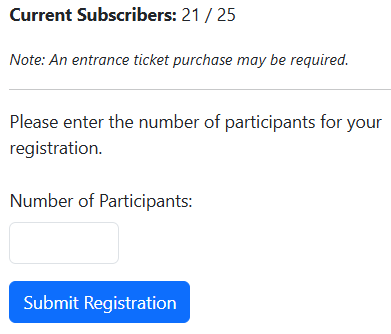
\includegraphics[width=\textwidth, keepaspectratio]{capitoli/immagini/p18.png}
        \caption{V1 (Prima)}
    \end{subfigure}
    \hfill
    \begin{subfigure}[b]{0.4\textwidth}
        \centering
        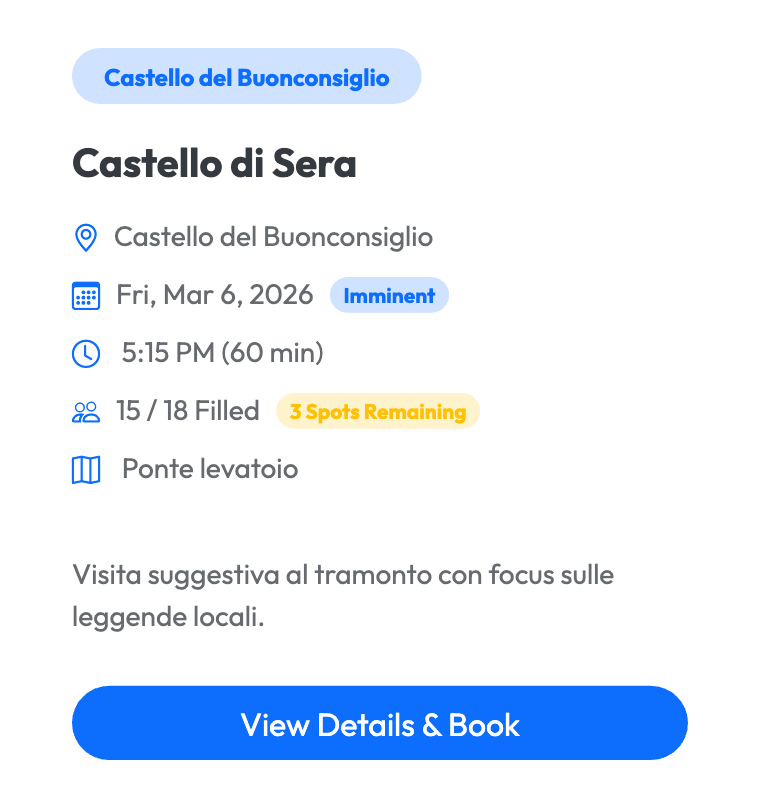
\includegraphics[width=\textwidth, keepaspectratio]{capitoli/immagini/v2/p20_v2.png}
        \caption{V2 (Dopo)}
    \end{subfigure}
    \caption{P.20 -- Posti disponibili: V1 (nessun indicatore) vs V2 (contatore "(X spots remaining)" esplicito).}
    \label{fig:det_p20}
\end{figure}

\noindent\textbf{P.21 \& P.22 -- Ridondanza informativa Register} \hfill \textit{Severità: 1}

La pagina di registrazione aveva link multipli verso il login e spiegazioni dei ruoli non necessarie. In V2 il form è semplificato: un solo link "Already have an account? Login" e nessuna descrizione dei ruoli.

\begin{figure}[H]
    \centering
    \begin{subfigure}[b]{0.47\textwidth}
        \centering
        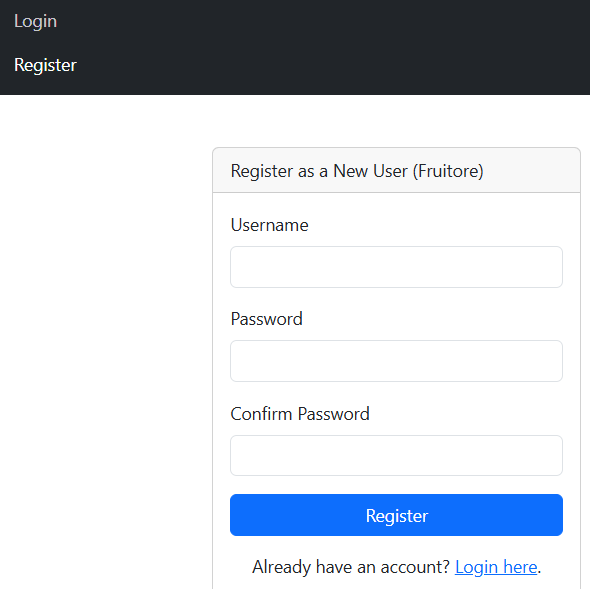
\includegraphics[width=\textwidth, keepaspectratio]{capitoli/immagini/p19.png}
        \caption{V1 (Prima)}
    \end{subfigure}
    \hfill
    \begin{subfigure}[b]{0.47\textwidth}
        \centering
        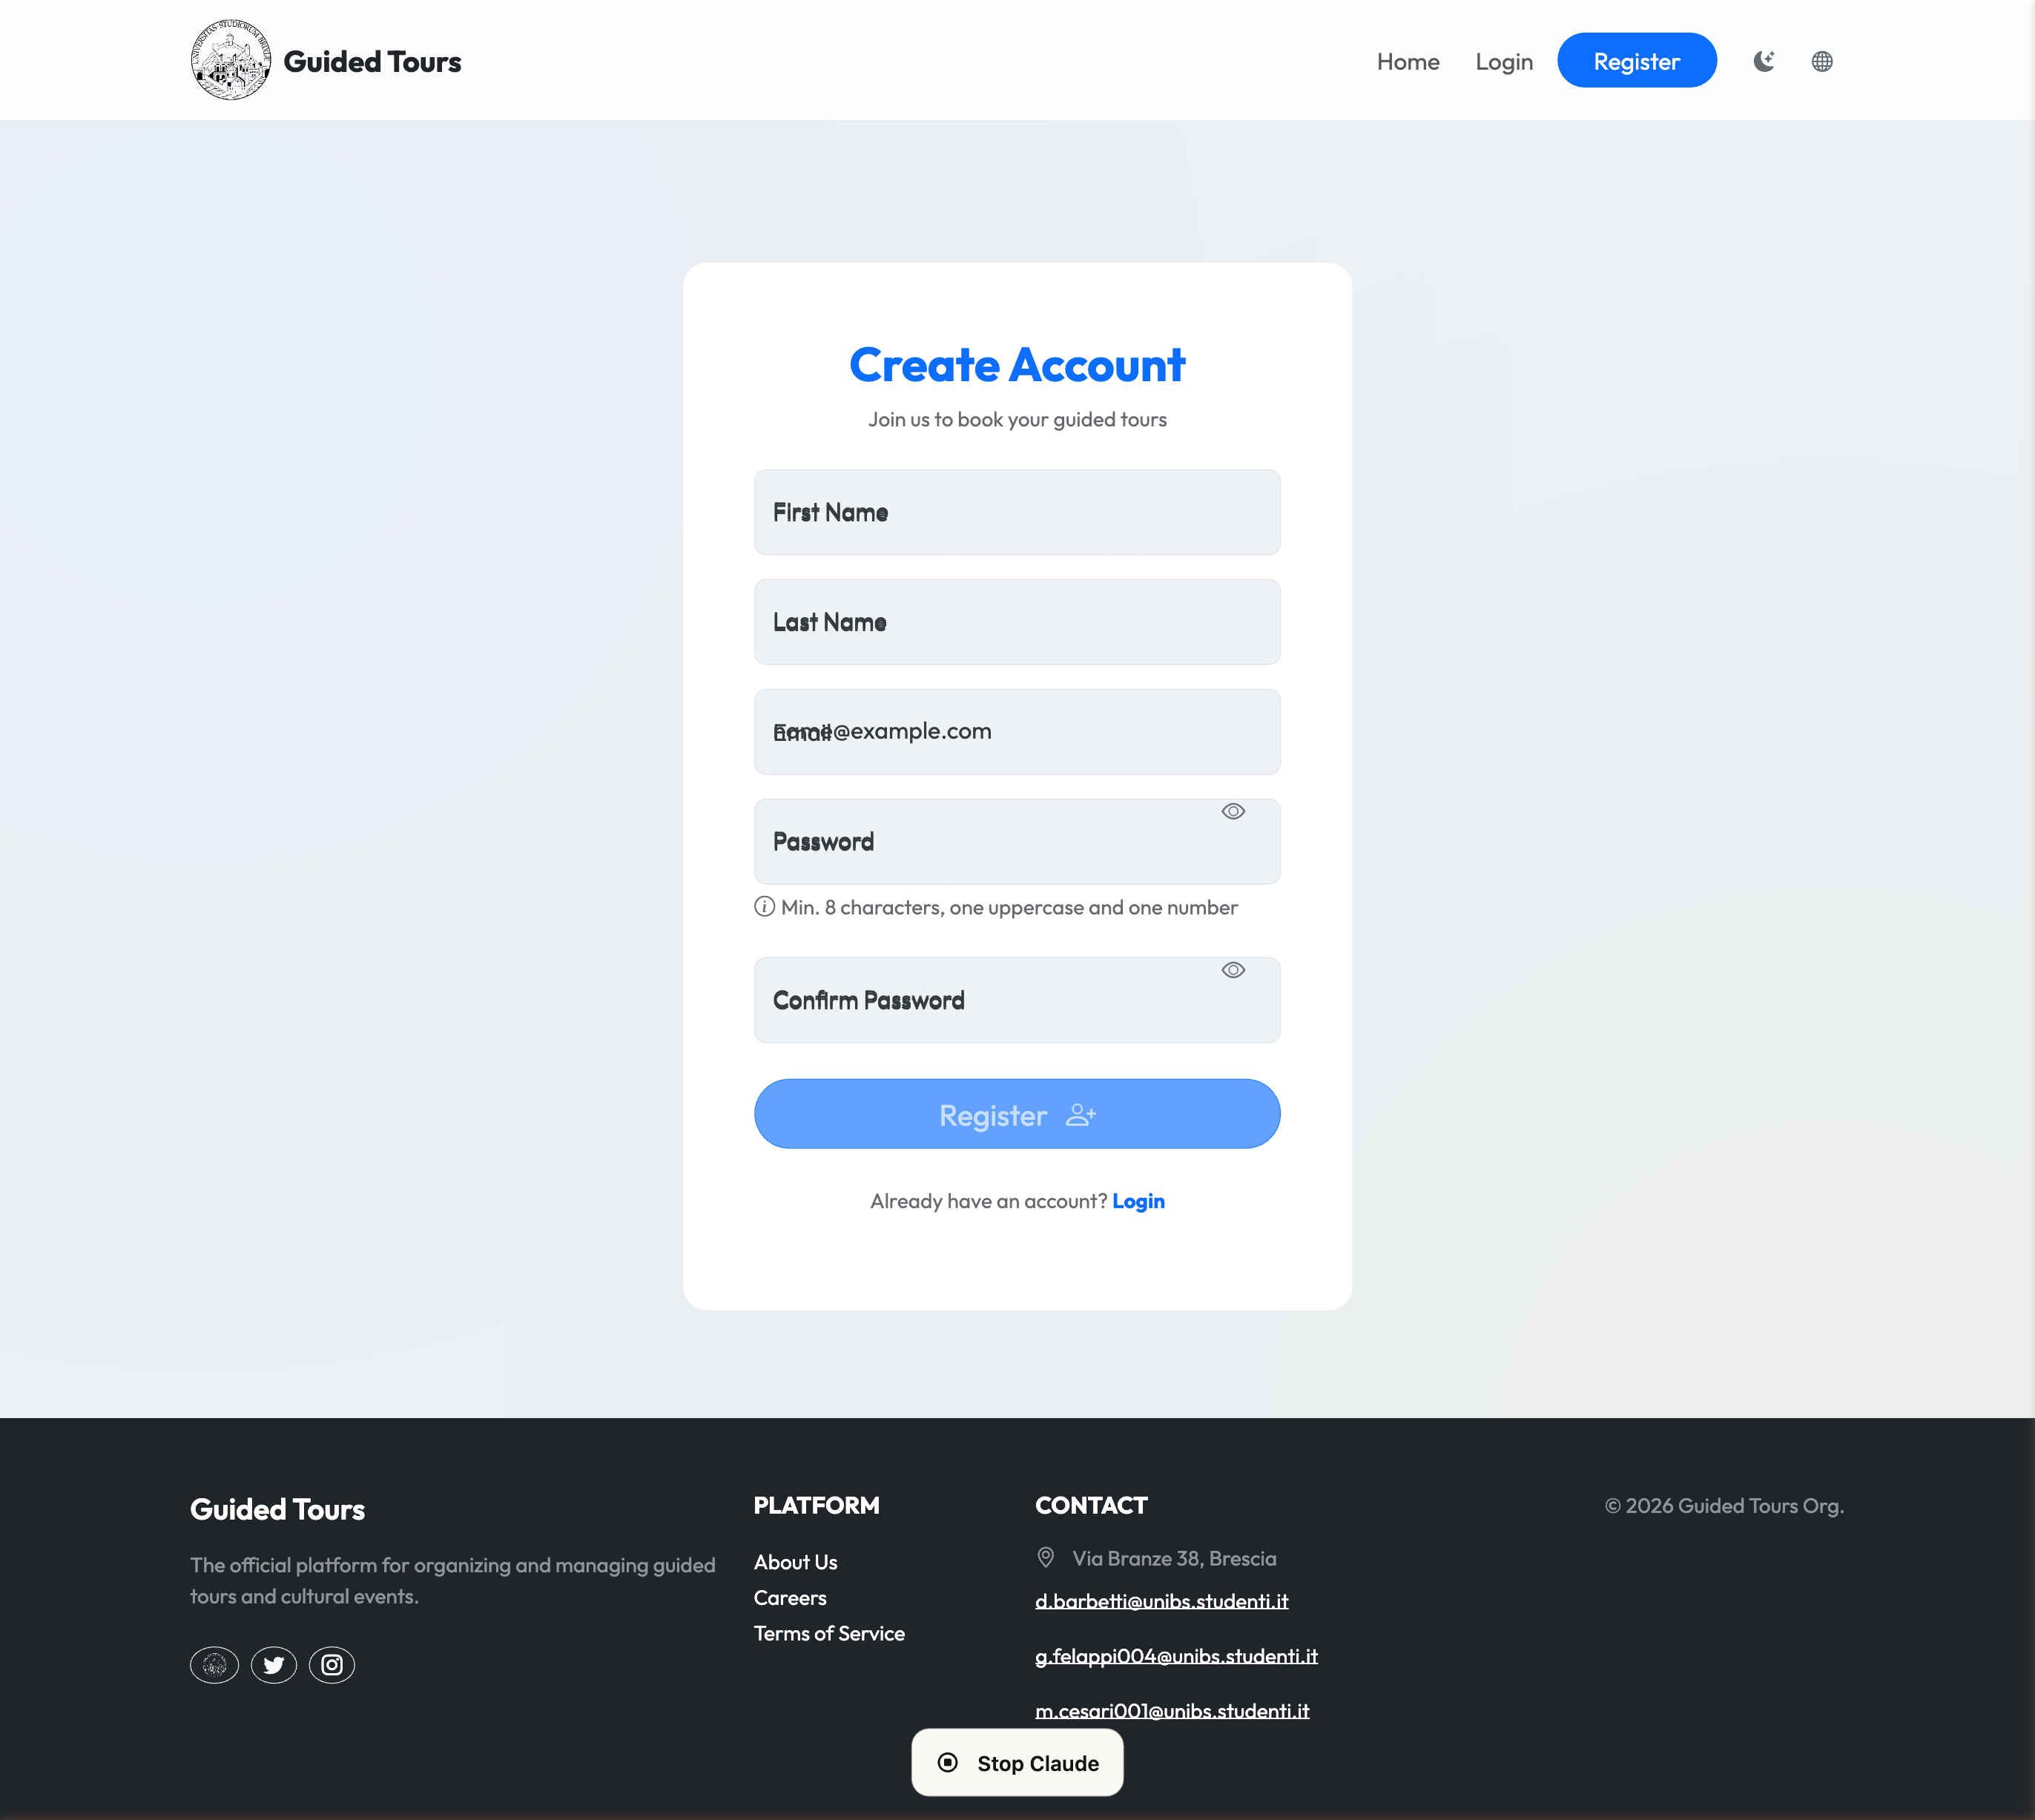
\includegraphics[width=\textwidth, keepaspectratio]{capitoli/immagini/v2/p21_v2.png}
        \caption{V2 (Dopo)}
    \end{subfigure}
    \caption{P.21/P.22 -- Register: V1 (link ridondanti e testo sui ruoli) vs V2 (form essenziale).}
    \label{fig:det_p21}
\end{figure}

\noindent\textbf{P.23 -- Validazione tardiva input} \hfill \textit{Severità: 2}

La validazione della password avveniva solo al submit. In V2 script JavaScript forniscono feedback visivo in tempo reale durante la digitazione: lunghezza minima e corrispondenza tra i due campi.

\begin{figure}[H]
    \centering
    \begin{subfigure}[b]{0.47\textwidth}
        \centering
        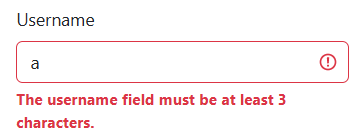
\includegraphics[width=\textwidth, keepaspectratio]{capitoli/immagini/p21.png}
        \caption{V1 (Prima)}
    \end{subfigure}
    \hfill
    \begin{subfigure}[b]{0.47\textwidth}
        \centering
        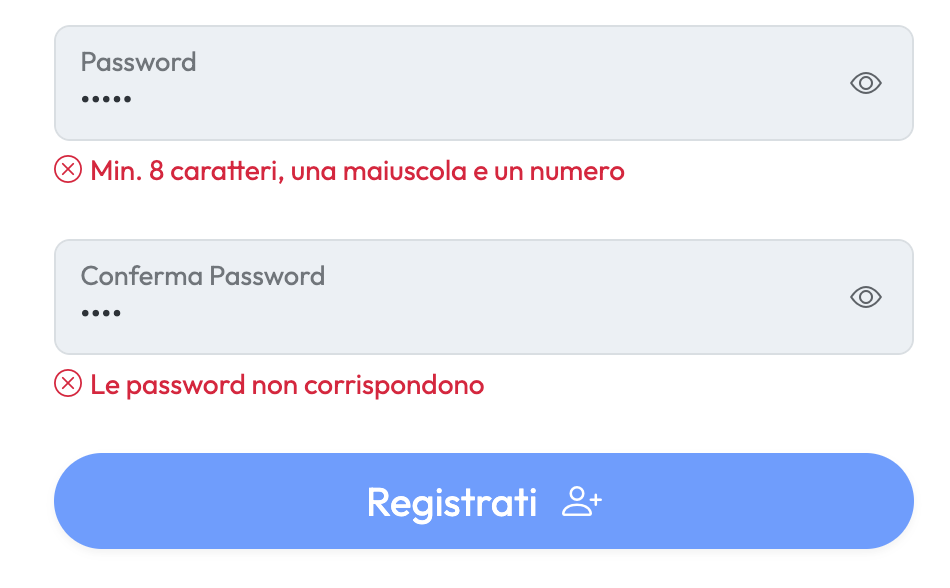
\includegraphics[width=\textwidth, keepaspectratio]{capitoli/immagini/v2/p23_v2.png}
        \caption{V2 (Dopo)}
    \end{subfigure}
    \caption{P.23 -- Validazione live: V1 (nessun feedback) vs V2 (indicatori real-time di lunghezza e match password).}
    \label{fig:det_p23}
\end{figure}

\subsection{Dashboard Fruitore}

\noindent\textbf{P.24 -- Visibilità "Booking code"} \hfill \textit{Severità: 1}

Il codice di prenotazione era presentato senza enfasi visiva. In V2 è visualizzato in font monospaziato bold con etichetta "Booking Code" esplicita.

\begin{figure}[H]
    \centering
    \begin{subfigure}[b]{0.47\textwidth}
        \centering
        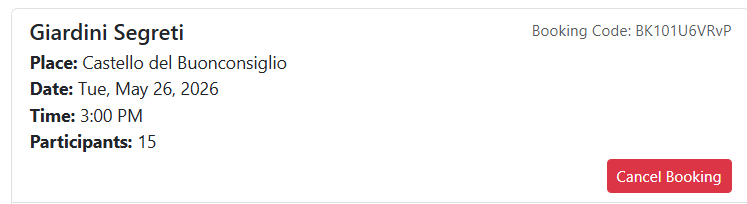
\includegraphics[width=\textwidth, keepaspectratio]{capitoli/immagini/p22.png}
        \caption{V1 (Prima)}
    \end{subfigure}
    \hfill
    \begin{subfigure}[b]{0.47\textwidth}
        \centering
        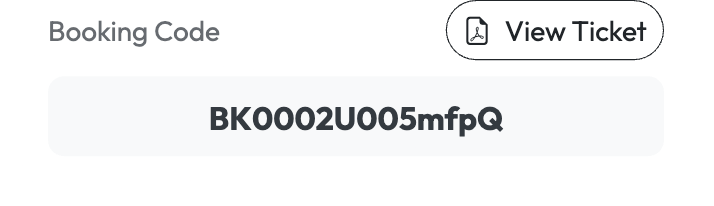
\includegraphics[width=\textwidth, keepaspectratio]{capitoli/immagini/v2/p24_v2.png}
        \caption{V2 (Dopo)}
    \end{subfigure}
    \caption{P.24 -- Booking code: V1 (testo generico) vs V2 (font monospaziato bold con etichetta esplicita).}
    \label{fig:det_p24}
\end{figure}

\noindent\textbf{P.25 -- Ambiguità etichetta "Participant"} \hfill \textit{Severità: 2}

L'etichetta non chiariva se indicasse il gruppo dell'utente o il totale della visita. In V2 è standardizzata in "X Participants".

\begin{figure}[H]
    \centering
    \begin{subfigure}[b]{0.47\textwidth}
        \centering
        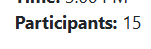
\includegraphics[width=\textwidth, keepaspectratio]{capitoli/immagini/p23.png}
        \caption{V1 (Prima)}
    \end{subfigure}
    \hfill
    \begin{subfigure}[b]{0.47\textwidth}
        \centering
        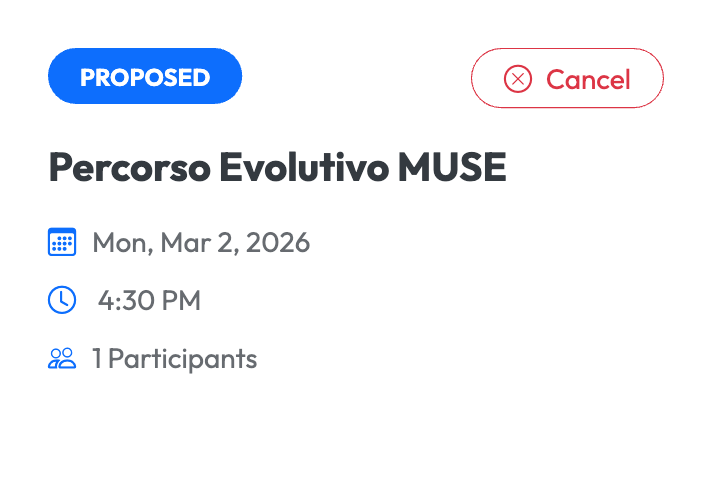
\includegraphics[width=\textwidth, keepaspectratio]{capitoli/immagini/v2/p25_v2.png}
        \caption{V2 (Dopo)}
    \end{subfigure}
    \caption{P.25 -- Etichetta partecipanti: V1 (ambigua) vs V2 (standardizzata "X Participants").}
    \label{fig:det_p25}
\end{figure}

\noindent\textbf{P.26 -- Affordance ingannevole "My Booking"} \hfill \textit{Severità: 2}

Il menu a tendina suggeriva interattività che non portava ad azioni utili. In V2 è sostituito da un bottone esplicito "Cancel Booking" con modale di conferma.

\begin{figure}[H]
    \centering
    \begin{subfigure}[b]{0.47\textwidth}
        \centering
        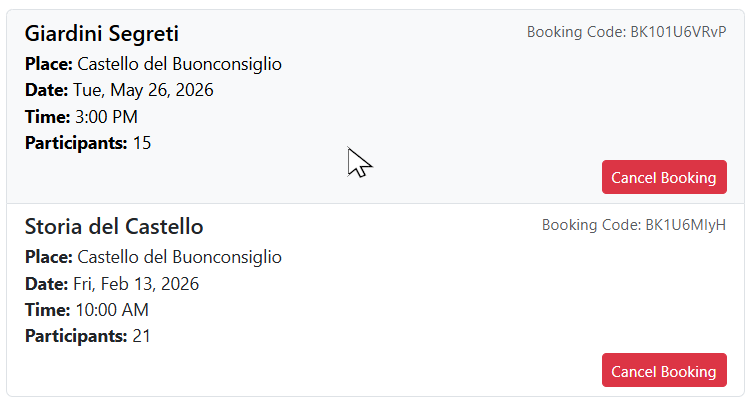
\includegraphics[width=\textwidth, keepaspectratio]{capitoli/immagini/p24.png}
        \caption{V1 (Prima)}
    \end{subfigure}
    \hfill
    \begin{subfigure}[b]{0.47\textwidth}
        \centering
        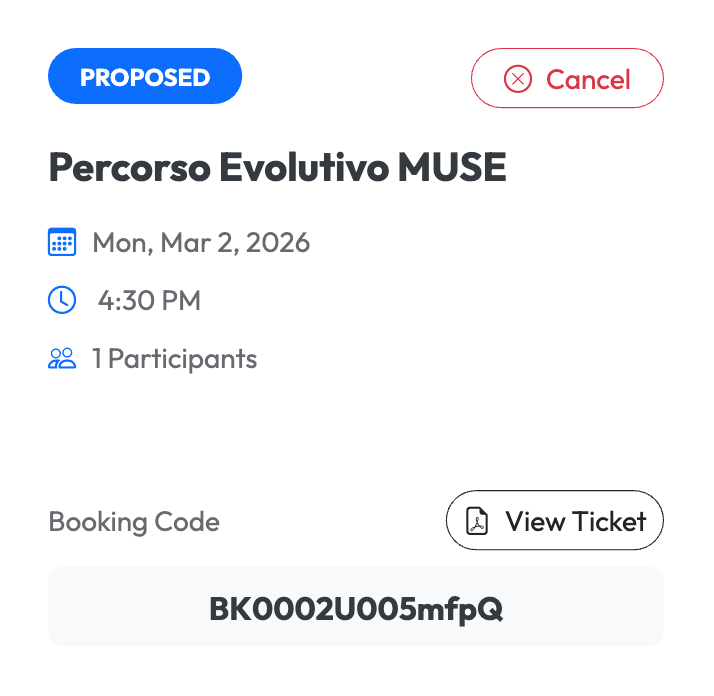
\includegraphics[width=\textwidth, keepaspectratio]{capitoli/immagini/v2/p26_v2.png}
        \caption{V2 (Dopo)}
    \end{subfigure}
    \caption{P.26 -- Affordance: V1 (menu ambiguo) vs V2 (bottone "Cancel Booking" con modale).}
    \label{fig:det_p26}
\end{figure}

\noindent\textbf{P.27 -- Stile pulsante eliminazione} \hfill \textit{Severità: 1}

Il bottone di cancellazione non comunicava la pericolosità dell'azione. In V2 adotta \texttt{btn-danger} con testo rosso, coerente con il Design System per azioni distruttive.

\begin{figure}[H]
    \centering
    \begin{minipage}[c]{0.63\textwidth}
        \centering
        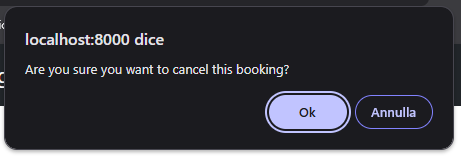
\includegraphics[width=\textwidth, keepaspectratio]{capitoli/immagini/p25.png}
        \par\small\textit{V1 -- stile neutro}
    \end{minipage}
    \hfill
    \begin{minipage}[c]{0.30\textwidth}
        \centering
        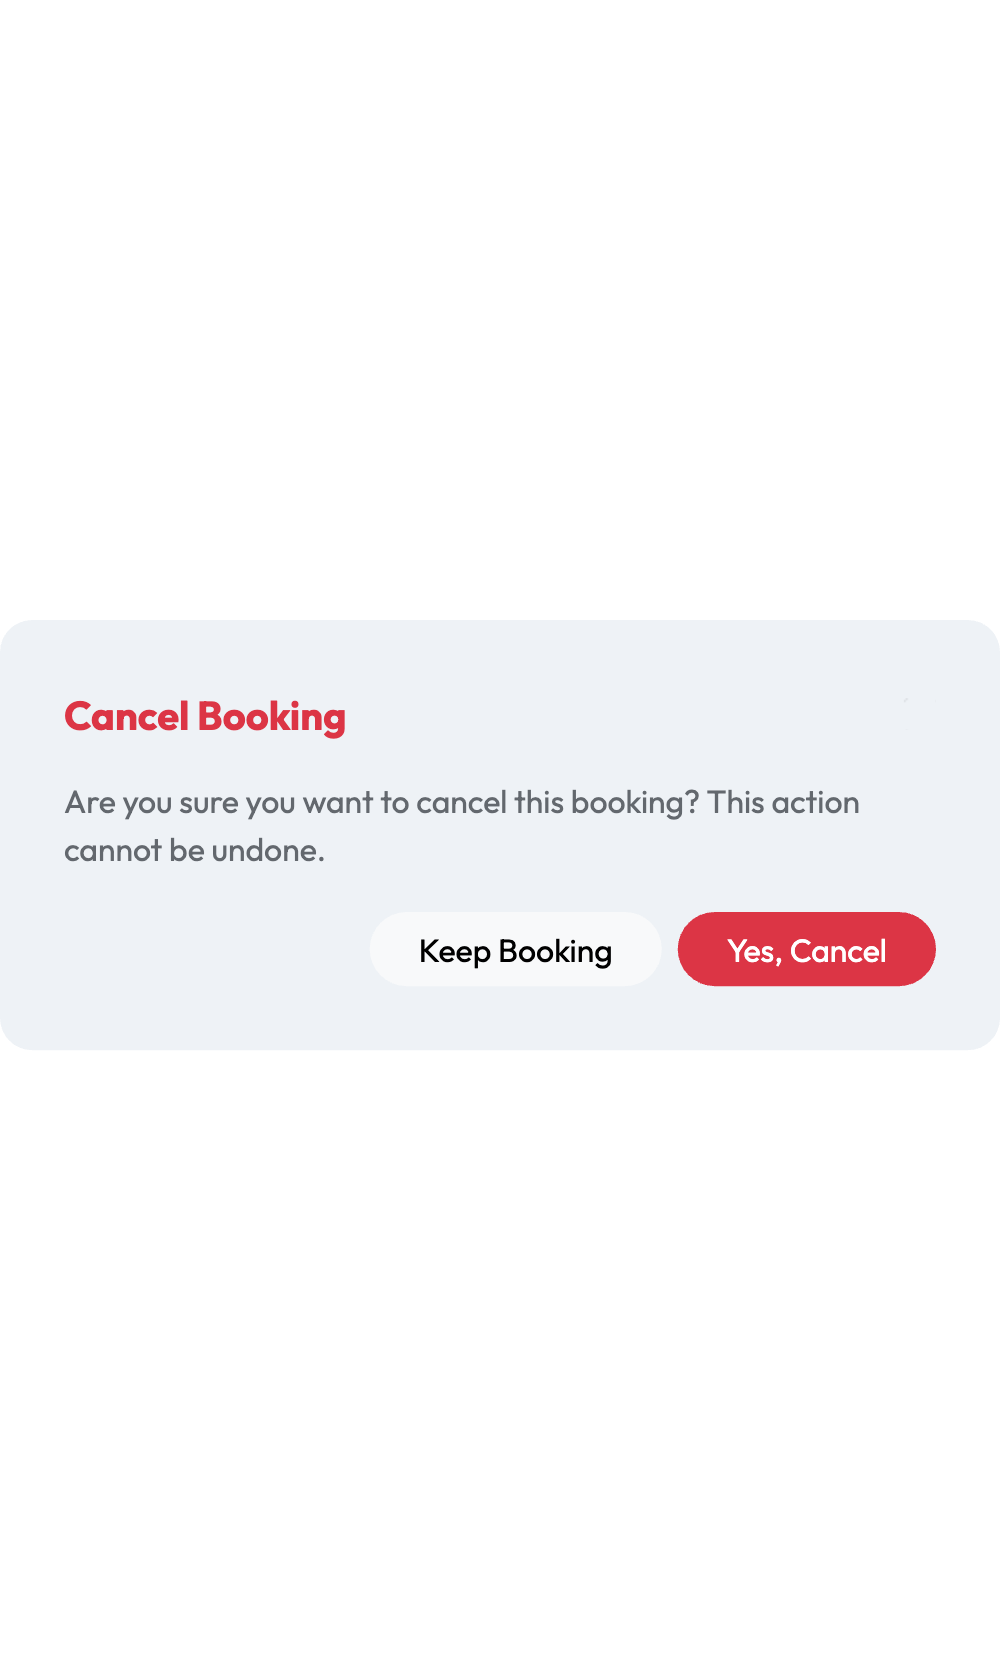
\includegraphics[width=\textwidth, keepaspectratio]{capitoli/immagini/v2/p27_v2.png}
        \par\small\textit{V2 -- \texttt{btn-danger} rosso}
    \end{minipage}
    \caption{P.27 -- Stile bottone: V1 (stile neutro) vs V2 (\texttt{btn-danger} rosso coerente).}
    \label{fig:det_p27}
\end{figure}

\newpage
\subsection{Area Amministratore}

\noindent\textbf{P.28 -- Inconsistenza terminologica} \hfill \textit{Severità: 1}

"Tour", "Visit" e "Booking" erano usati in modo intercambiabile. In V2 la convenzione è: "Tours/Bookings" lato utente finale, "Visits" lato amministrativo.


\noindent\textbf{P.29 -- Incoerenza spaziatura Header} \hfill \textit{Severità: 1}

Le spaziature tra header e contenuto variavano tra le pagine. In V2 la Navbar Bootstrap garantisce padding uniformi in tutta l'applicazione.

\begin{figure}[H]
    \centering
    
\includegraphics[width=0.85\textwidth, keepaspectratio]{capitoli/immagini/p27.png}\\[0.6em]
    
\includegraphics[width=0.85\textwidth, keepaspectratio]{capitoli/immagini/v2/p29_v2.png}
    \caption{P.29 -- Spaziatura header: V1 sopra (padding irregolare) vs V2 sotto (navbar con spaziatura uniforme).}
    \label{fig:det_p29}
\end{figure}

\noindent\textbf{P.30 -- Validazione tardiva aggiunta utente} \hfill \textit{Severità: 2}

Nel modale di creazione utente la validazione avveniva solo al submit. In V2 feedback JavaScript live verifica la password direttamente nel modale amministrativo.

\begin{figure}[H]
    \centering
    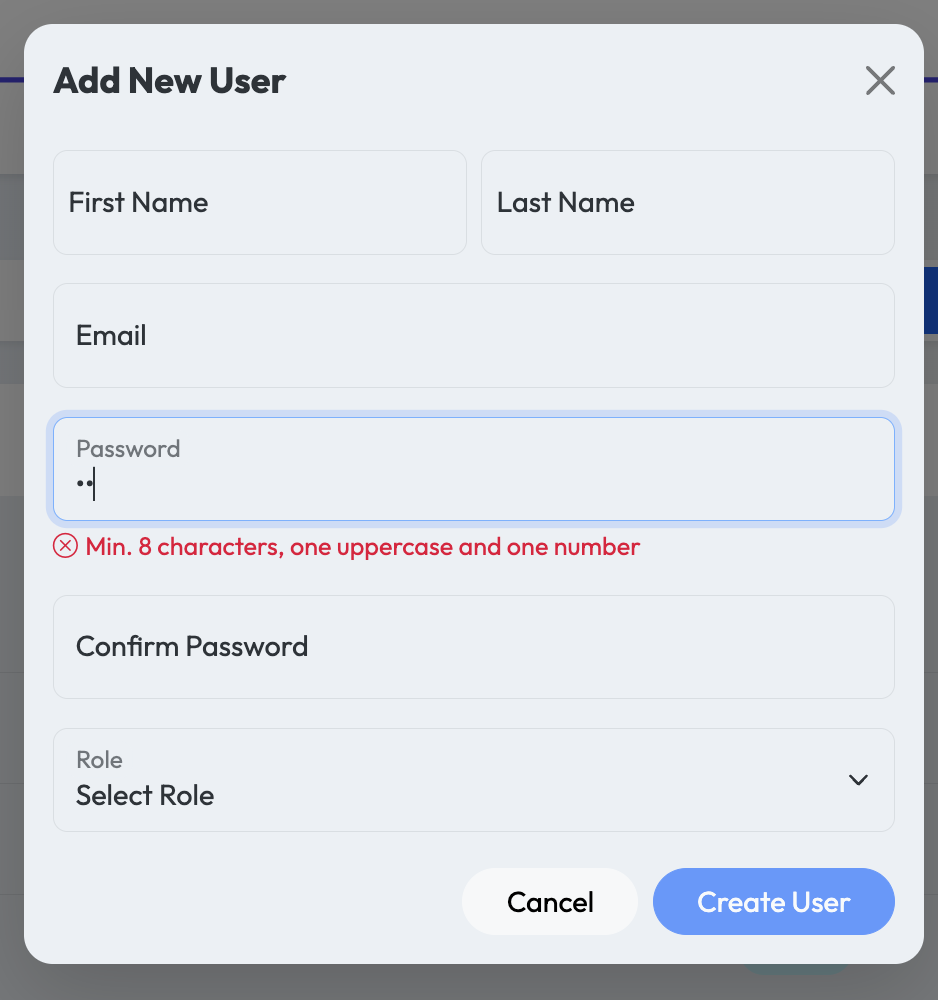
\includegraphics[width=0.40\textwidth, keepaspectratio]{capitoli/immagini/v2/p30_v2.png}
    \caption{P.30 -- Validazione live nel modale admin: indicatori real-time per la password nel configuratore.}
    \label{fig:det_p30}
\end{figure}

\noindent\textbf{P.31 -- Assenza conferma eliminazione} \hfill \textit{Severità: 4}

La criticità più grave del sistema: ogni eliminazione avveniva immediatamente al click. In V2 il Global Delete Confirmation Modal interrompe l'azione e obbliga a una conferma esplicita con avviso "This action cannot be undone".

\begin{figure}[H]
    \centering
    \begin{subfigure}[b]{0.47\textwidth}
        \centering
        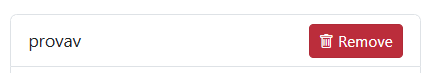
\includegraphics[width=\textwidth, keepaspectratio]{capitoli/immagini/p29.png}
        \caption{V1 (Prima)}
    \end{subfigure}
    \hfill
    \begin{subfigure}[b]{0.47\textwidth}
        \centering
        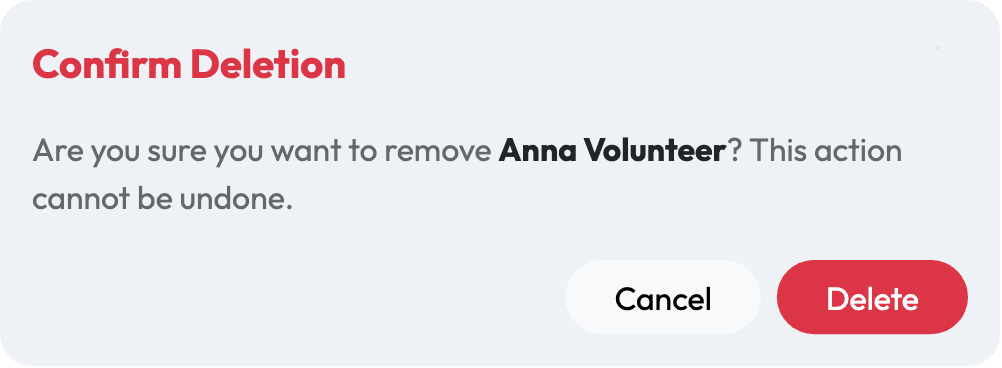
\includegraphics[width=\textwidth, keepaspectratio]{capitoli/immagini/v2/p31_v2.png}
        \caption{V2 (Dopo)}
    \end{subfigure}
    \caption{P.31 -- Conferma eliminazione: V1 (eliminazione immediata) vs V2 (Global Delete Modal).}
    \label{fig:det_p31}
\end{figure}

\noindent\textbf{P.32 -- Disorganizzazione layout Visit Planning} \hfill \textit{Severità: 1}

Il pannello di pianificazione era caotico e difficile da navigare. In V2 le visite sono organizzate in card per mese con intestazioni chiare.

\begin{figure}[H]
    \centering
    \begin{subfigure}[b]{0.47\textwidth}
        \centering
        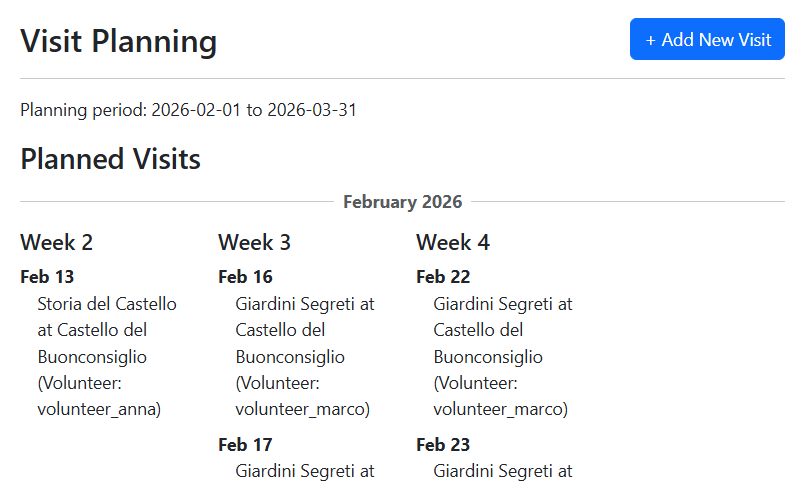
\includegraphics[width=\textwidth, keepaspectratio]{capitoli/immagini/p30.png}
        \caption{V1 (Prima)}
    \end{subfigure}
    \hfill
    \begin{subfigure}[b]{0.47\textwidth}
        \centering
        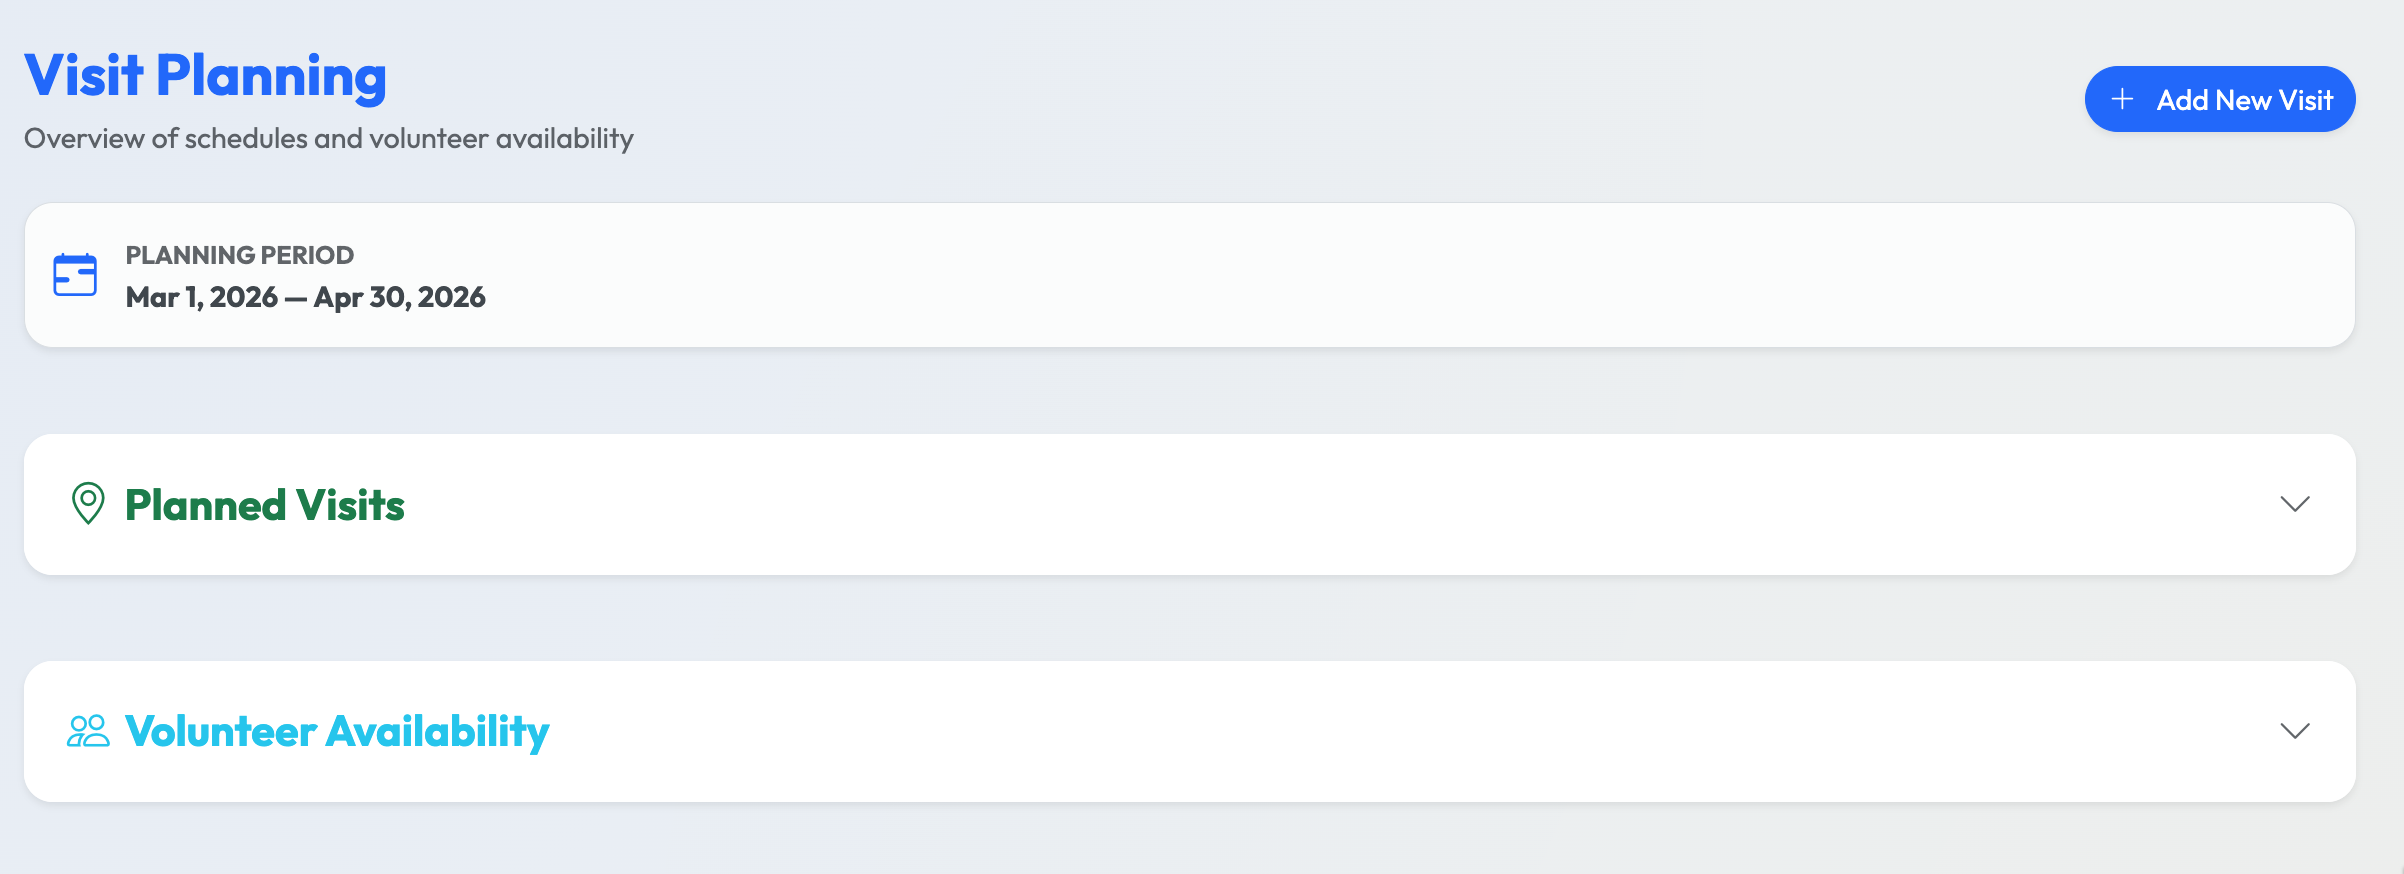
\includegraphics[width=\textwidth, keepaspectratio]{capitoli/immagini/v2/p32_v2.png}
        \caption{V2 (Dopo)}
    \end{subfigure}
    \caption{P.32 -- Visit Planning: V1 (layout disorganizzato) vs V2 (card mensili con sezioni chiare).}
    \label{fig:det_p32}
\end{figure}

\noindent\textbf{P.33 -- Flusso inserimento non intuitivo} \hfill \textit{Severità: 3}

La sequenza di inserimento di una nuova visita non era guidata. In V2 il form presenta un flusso step-by-step: Tipo Visita → Data → Volontario disponibile.

\begin{figure}[H]
    \centering
    \begin{subfigure}[b]{0.47\textwidth}
        \centering
        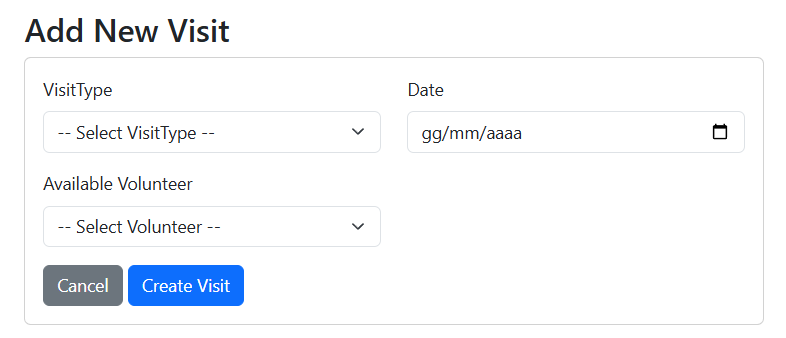
\includegraphics[width=\textwidth, keepaspectratio]{capitoli/immagini/p31.png}
        \caption{V1 (Prima)}
    \end{subfigure}
    \hfill
    \begin{subfigure}[b]{0.47\textwidth}
        \centering
        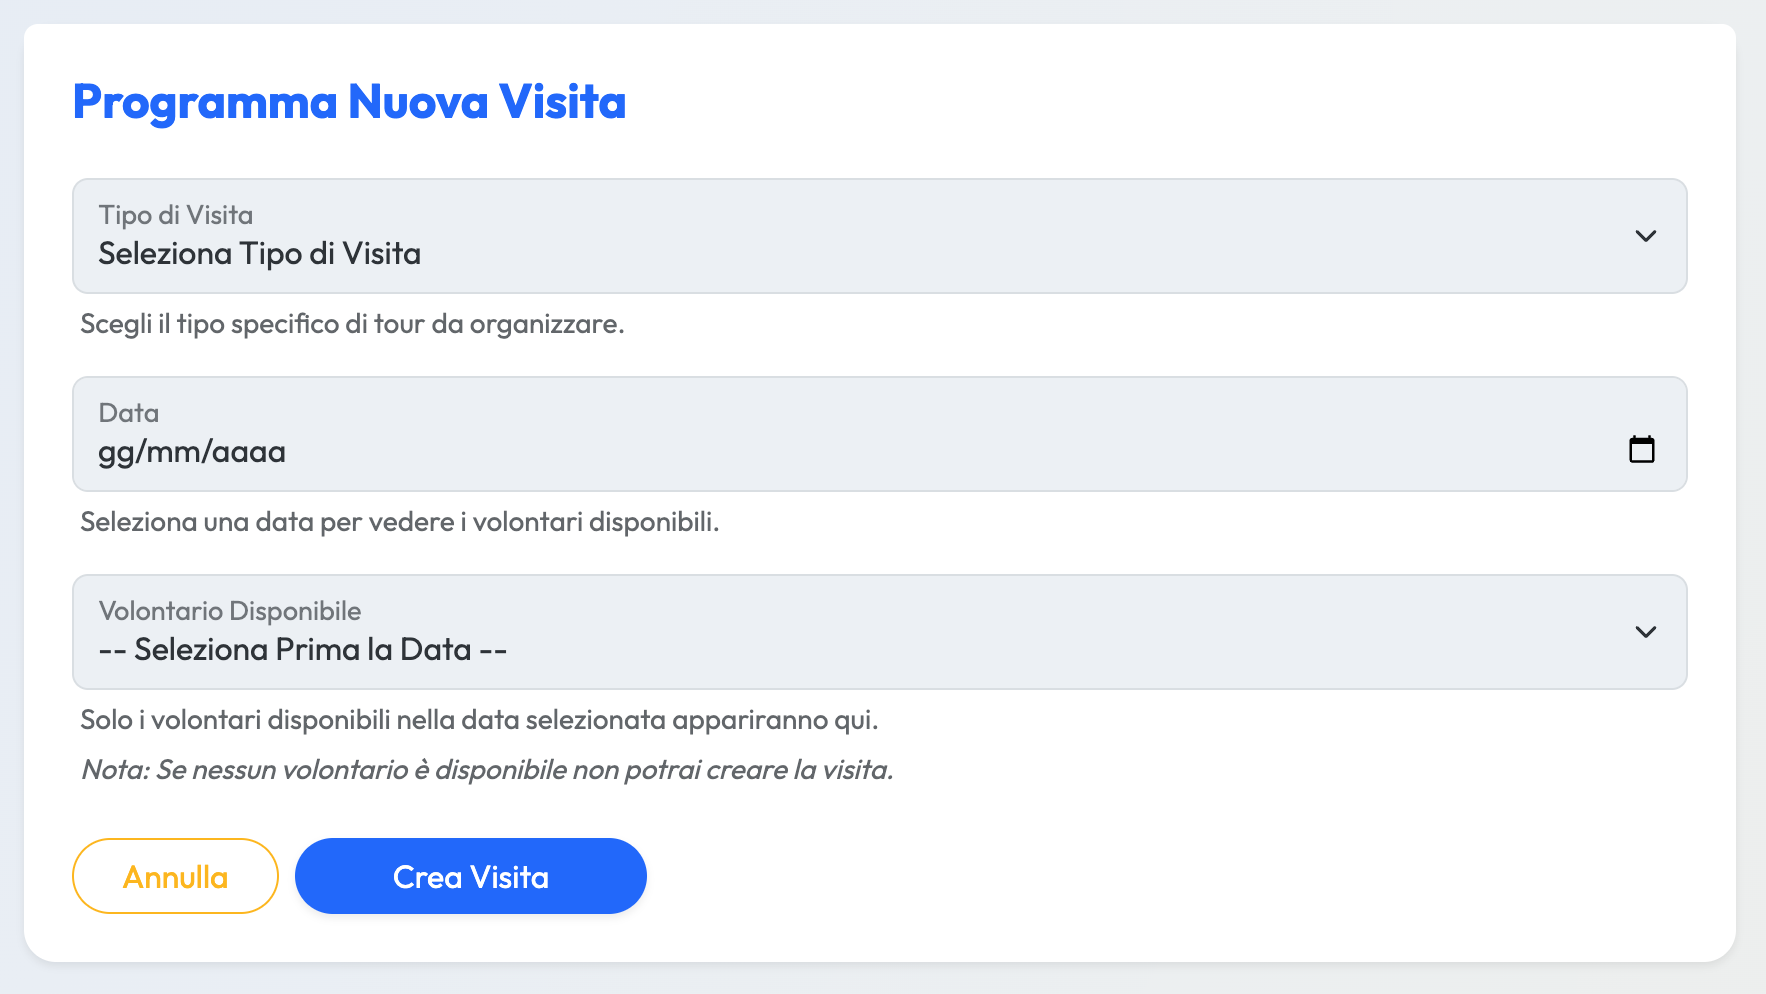
\includegraphics[width=\textwidth, keepaspectratio]{capitoli/immagini/v2/p33_v2.png}
        \caption{V2 (Dopo)}
    \end{subfigure}
    \caption{P.33 -- Add Visit: V1 (form non guidato) vs V2 (flusso Tipo → Data → Volontario).}
    \label{fig:det_p33}
\end{figure}

\noindent\textbf{P.34 -- Mancanza feedback su vincoli} \hfill \textit{Severità: 3}

L'utente non riceveva indicazioni sui vincoli procedurali prima del submit. In V2 help text contestuali appaiono accanto ai campi critici (data minima, assenza volontari disponibili).

\begin{figure}[H]
    \centering
    \begin{subfigure}[b]{0.47\textwidth}
        \centering
        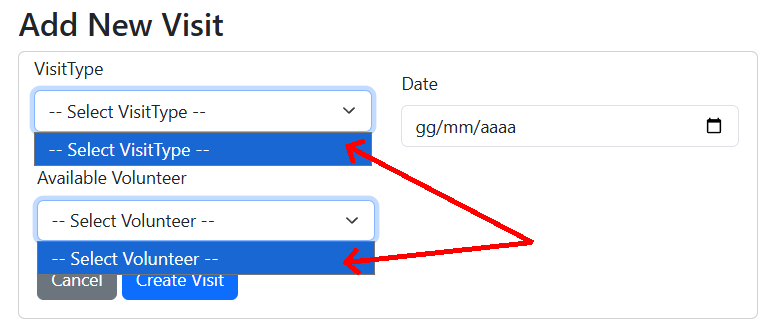
\includegraphics[width=\textwidth, keepaspectratio]{capitoli/immagini/p32.png}
        \caption{V1 (Prima)}
    \end{subfigure}
    \hfill
    \begin{subfigure}[b]{0.47\textwidth}
        \centering
        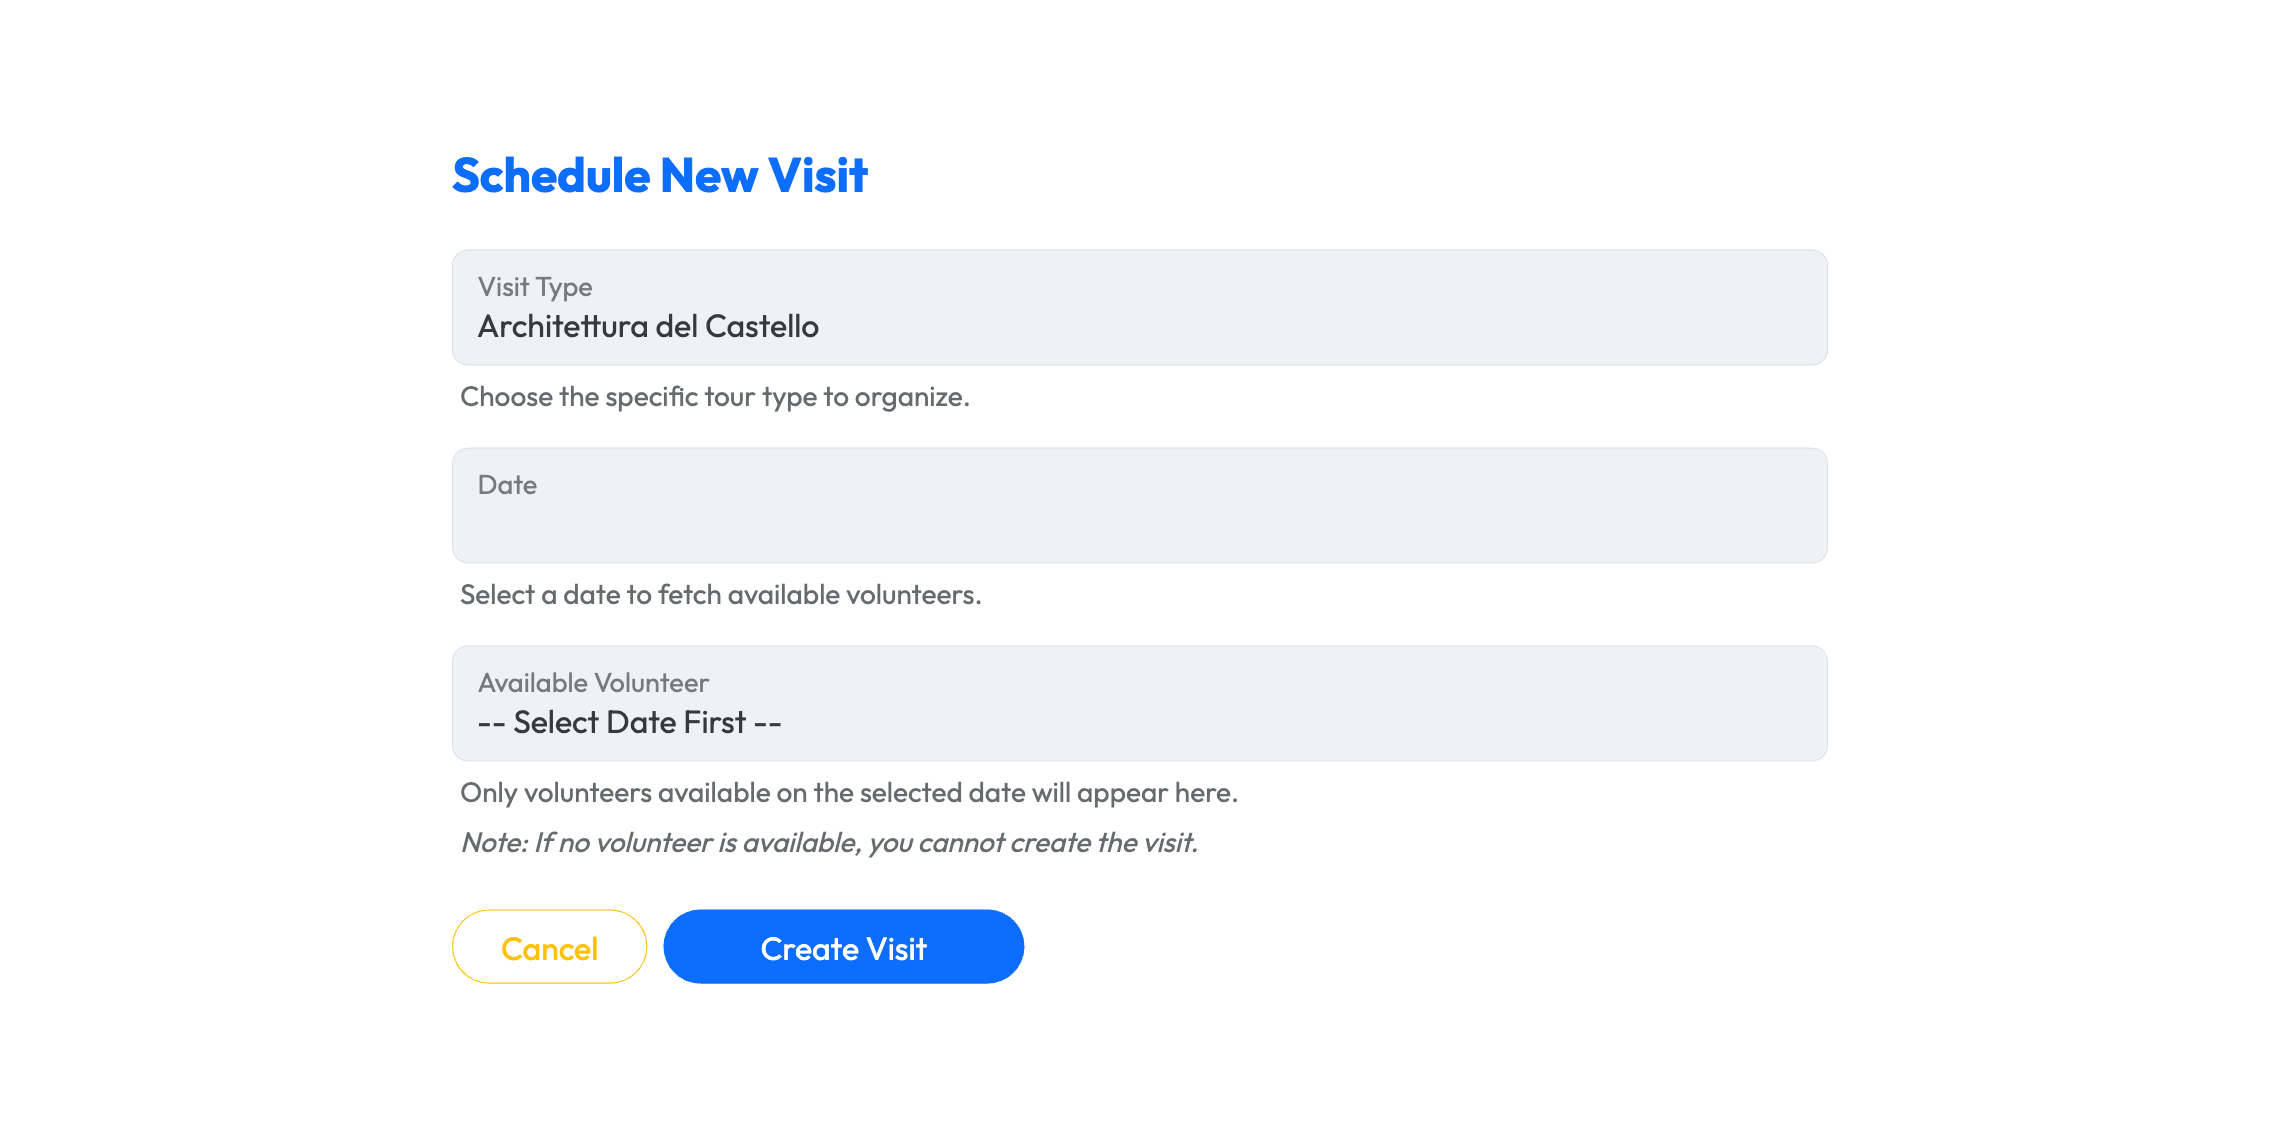
\includegraphics[width=\textwidth, keepaspectratio]{capitoli/immagini/v2/p34_v2.png}
        \caption{V2 (Dopo)}
    \end{subfigure}
    \caption{P.34 -- Feedback vincoli: V1 (nessun help text) vs V2 (indicazioni contestuali accanto ai campi).}
    \label{fig:det_p34}
\end{figure}

\noindent\textbf{P.40 -- Colore bottone non coerente} \hfill \textit{Severità: 2}

Il bottone "Change Password" nella pagina profilo usava il rosso, colore semanticamente associato al pericolo. In V2 è allineato al Design System con uno stile neutro.

\begin{figure}[H]
    \centering
    \begin{subfigure}[b]{0.47\textwidth}
        \centering
        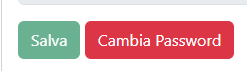
\includegraphics[width=\textwidth, keepaspectratio]{capitoli/immagini/p34.png}
        \caption{V1 (Prima)}
    \end{subfigure}
    \hfill
    \begin{subfigure}[b]{0.47\textwidth}
        \centering
        
\includegraphics[width=\textwidth, keepaspectratio]{capitoli/immagini/v2/p40_v2.png}
        \caption{V2 (Dopo)}
    \end{subfigure}
    \caption{P.40 -- Bottone profilo: V1 (rosso fuorviante) vs V2 (stile neutro coerente).}
    \label{fig:det_p40}
\end{figure}

\newpage
\subsection{Area Volontario (Guida)}

\noindent\textbf{P.37 -- Assenza indicazioni operative} \hfill \textit{Severità: 2}

Le guide non disponevano di promemoria operativi nella pagina delle visite assegnate. In V2 un banner \texttt{alert-info} fornisce istruzioni specifiche: puntualità, verifica booking code, gestione biglietti e contatto organizzativo in caso di imprevisti.

\begin{figure}[H]
    \centering
    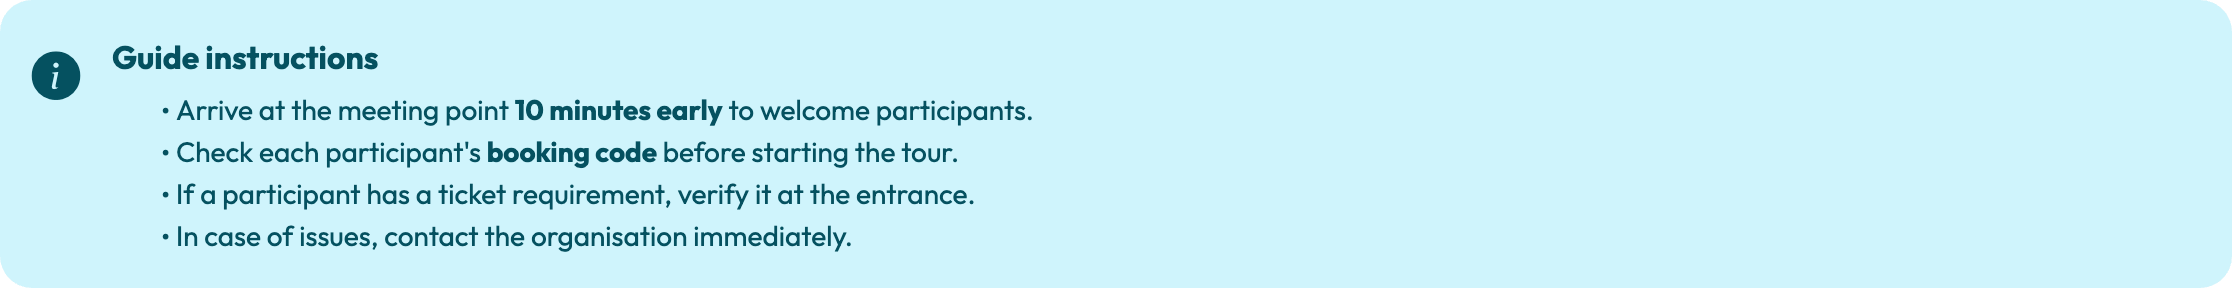
\includegraphics[width=0.85\textwidth, keepaspectratio]{capitoli/immagini/v2/p37_v2.png}
    \caption{P.37 -- Banner istruzioni: V2 con promemoria operativo nella pagina "My Assigned Visits".}
    \label{fig:det_p37}
\end{figure}

\noindent\textbf{P.38 -- Ridondanza nome volontario nelle card} \hfill \textit{Severità: 1}

Il nome del volontario assegnato compariva sempre, anche nella vista privata della guida stessa. In V2 il nome è nascosto se coincide con l'utente loggato, visibile solo ad altri ruoli.

\begin{figure}[H]
    \centering
    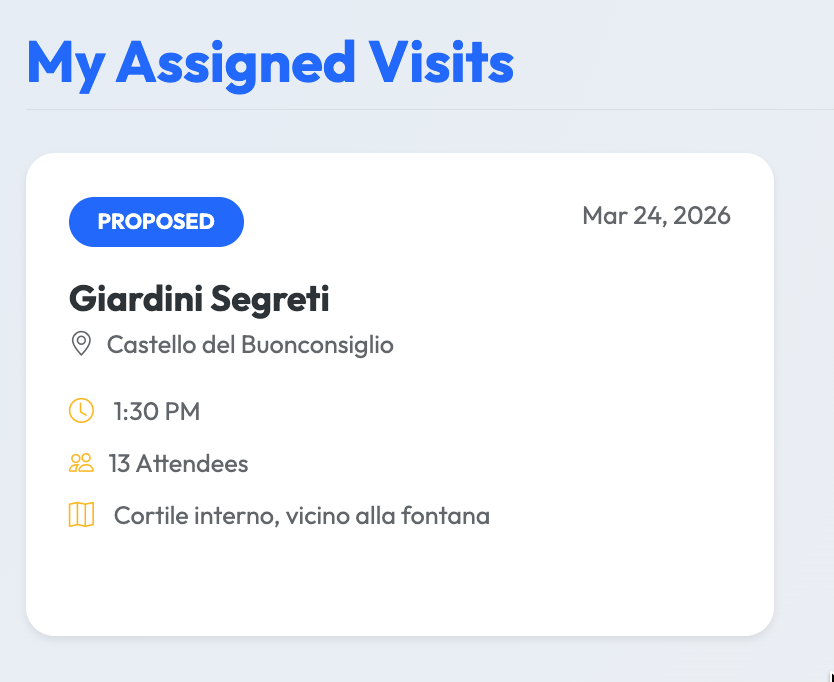
\includegraphics[width=0.55\textwidth, keepaspectratio]{capitoli/immagini/v2/p38_v2.png}
    \caption{P.38 -- Ridondanza nome: V2 -- il nome del volontario è nascosto quando coincide con l'utente corrente.}
    \label{fig:det_p38}
\end{figure}

% ─────────────────────────────────────────────────────────────────────────────
\section{Problemi Non Risolti}
\label{sec:problemi_aperti}

Cinque problemi identificati nel Capitolo 3 non sono stati risolti nella presente versione del sistema. In tutti i casi la decisione è motivata da complessità implementativa, vincoli di scope del progetto o dalla bassa severità rapportata all'impatto atteso sull'esperienza d'uso. Tali problemi restano candidati prioritari per iterazioni future.

\begin{table}[H]
\centering
\renewcommand{\arraystretch}{1.5}
\small
\begin{tabularx}{\textwidth}{|c|X|c|X|}
\hline
\textbf{P\#} & \textbf{Problema} & \textbf{Sev.} & \textbf{Motivazione della mancata risoluzione} \\ \hline
1  & Cursore non coerente su elementi cliccabili & 2 & Richiede un audit sistematico di tutti gli elementi interattivi dell'interfaccia con aggiunta di \texttt{cursor: pointer} nei CSS globali. Il rischio di regressioni stilistiche ha portato a posticipare l'intervento. \\ \hline
2  & Assenza notifica rischio annullamento visita & 3 & Necessita di logica server-side per confrontare partecipanti iscritti e soglia minima, con generazione di alert contestuali nella dashboard. Fuori dallo scope della riprogettazione corrente. \\ \hline
36 & Mancanza selezione multipla nel calendario  & 2 & Richiederebbe un refactoring significativo del componente JavaScript del calendario disponibilità (shortcut "Tutti i weekend" / "Tutto il mese"). Identificato come miglioramento futuro ad alta priorità. \\ \hline
39 & Messaggio stato vuoto senza Call to Action  & 2 & La funzionalità principale rimane intatta; la CTA verso la Homepage sarà integrata in un rilascio successivo a basso rischio. \\ \hline
—  & Scroll inaspettato al cambio pagina         & — & Comportamento collaterale del pattern "Load More" asincrono: la chiamata a \texttt{scrollIntoView()} si comporta diversamente a seconda del browser. Richiede refactoring della logica di scroll nel componente Alpine.js. \\ \hline
\end{tabularx}
\caption{Problemi identificati nel Capitolo 3 non risolti nella versione corrente.}
\label{tab:problemi_aperti}
\end{table}
